% Options for packages loaded elsewhere
\PassOptionsToPackage{unicode}{hyperref}
\PassOptionsToPackage{hyphens}{url}
%
\documentclass[
  12pt,
  a4paper,
  DIV=11,
  numbers=noendperiod]{scrreprt}

\usepackage{amsmath,amssymb}
\usepackage{setspace}
\usepackage{iftex}
\ifPDFTeX
  \usepackage[T1]{fontenc}
  \usepackage[utf8]{inputenc}
  \usepackage{textcomp} % provide euro and other symbols
\else % if luatex or xetex
  \usepackage{unicode-math}
  \defaultfontfeatures{Scale=MatchLowercase}
  \defaultfontfeatures[\rmfamily]{Ligatures=TeX,Scale=1}
\fi
\usepackage{lmodern}
\ifPDFTeX\else  
    % xetex/luatex font selection
\fi
% Use upquote if available, for straight quotes in verbatim environments
\IfFileExists{upquote.sty}{\usepackage{upquote}}{}
\IfFileExists{microtype.sty}{% use microtype if available
  \usepackage[]{microtype}
  \UseMicrotypeSet[protrusion]{basicmath} % disable protrusion for tt fonts
}{}
\usepackage{xcolor}
\usepackage{svg}
\setlength{\emergencystretch}{3em} % prevent overfull lines
\setcounter{secnumdepth}{5}
% Make \paragraph and \subparagraph free-standing
\ifx\paragraph\undefined\else
  \let\oldparagraph\paragraph
  \renewcommand{\paragraph}[1]{\oldparagraph{#1}\mbox{}}
\fi
\ifx\subparagraph\undefined\else
  \let\oldsubparagraph\subparagraph
  \renewcommand{\subparagraph}[1]{\oldsubparagraph{#1}\mbox{}}
\fi

\usepackage{color}
\usepackage{fancyvrb}
\newcommand{\VerbBar}{|}
\newcommand{\VERB}{\Verb[commandchars=\\\{\}]}
\DefineVerbatimEnvironment{Highlighting}{Verbatim}{commandchars=\\\{\}}
% Add ',fontsize=\small' for more characters per line
\usepackage{framed}
\definecolor{shadecolor}{RGB}{241,243,245}
\newenvironment{Shaded}{\begin{snugshade}}{\end{snugshade}}
\newcommand{\AlertTok}[1]{\textcolor[rgb]{0.68,0.00,0.00}{#1}}
\newcommand{\AnnotationTok}[1]{\textcolor[rgb]{0.37,0.37,0.37}{#1}}
\newcommand{\AttributeTok}[1]{\textcolor[rgb]{0.40,0.45,0.13}{#1}}
\newcommand{\BaseNTok}[1]{\textcolor[rgb]{0.68,0.00,0.00}{#1}}
\newcommand{\BuiltInTok}[1]{\textcolor[rgb]{0.00,0.23,0.31}{#1}}
\newcommand{\CharTok}[1]{\textcolor[rgb]{0.13,0.47,0.30}{#1}}
\newcommand{\CommentTok}[1]{\textcolor[rgb]{0.37,0.37,0.37}{#1}}
\newcommand{\CommentVarTok}[1]{\textcolor[rgb]{0.37,0.37,0.37}{\textit{#1}}}
\newcommand{\ConstantTok}[1]{\textcolor[rgb]{0.56,0.35,0.01}{#1}}
\newcommand{\ControlFlowTok}[1]{\textcolor[rgb]{0.00,0.23,0.31}{#1}}
\newcommand{\DataTypeTok}[1]{\textcolor[rgb]{0.68,0.00,0.00}{#1}}
\newcommand{\DecValTok}[1]{\textcolor[rgb]{0.68,0.00,0.00}{#1}}
\newcommand{\DocumentationTok}[1]{\textcolor[rgb]{0.37,0.37,0.37}{\textit{#1}}}
\newcommand{\ErrorTok}[1]{\textcolor[rgb]{0.68,0.00,0.00}{#1}}
\newcommand{\ExtensionTok}[1]{\textcolor[rgb]{0.00,0.23,0.31}{#1}}
\newcommand{\FloatTok}[1]{\textcolor[rgb]{0.68,0.00,0.00}{#1}}
\newcommand{\FunctionTok}[1]{\textcolor[rgb]{0.28,0.35,0.67}{#1}}
\newcommand{\ImportTok}[1]{\textcolor[rgb]{0.00,0.46,0.62}{#1}}
\newcommand{\InformationTok}[1]{\textcolor[rgb]{0.37,0.37,0.37}{#1}}
\newcommand{\KeywordTok}[1]{\textcolor[rgb]{0.00,0.23,0.31}{#1}}
\newcommand{\NormalTok}[1]{\textcolor[rgb]{0.00,0.23,0.31}{#1}}
\newcommand{\OperatorTok}[1]{\textcolor[rgb]{0.37,0.37,0.37}{#1}}
\newcommand{\OtherTok}[1]{\textcolor[rgb]{0.00,0.23,0.31}{#1}}
\newcommand{\PreprocessorTok}[1]{\textcolor[rgb]{0.68,0.00,0.00}{#1}}
\newcommand{\RegionMarkerTok}[1]{\textcolor[rgb]{0.00,0.23,0.31}{#1}}
\newcommand{\SpecialCharTok}[1]{\textcolor[rgb]{0.37,0.37,0.37}{#1}}
\newcommand{\SpecialStringTok}[1]{\textcolor[rgb]{0.13,0.47,0.30}{#1}}
\newcommand{\StringTok}[1]{\textcolor[rgb]{0.13,0.47,0.30}{#1}}
\newcommand{\VariableTok}[1]{\textcolor[rgb]{0.07,0.07,0.07}{#1}}
\newcommand{\VerbatimStringTok}[1]{\textcolor[rgb]{0.13,0.47,0.30}{#1}}
\newcommand{\WarningTok}[1]{\textcolor[rgb]{0.37,0.37,0.37}{\textit{#1}}}

\providecommand{\tightlist}{%
  \setlength{\itemsep}{0pt}\setlength{\parskip}{0pt}}\usepackage{longtable,booktabs,array}
\usepackage{calc} % for calculating minipage widths
% Correct order of tables after \paragraph or \subparagraph
\usepackage{etoolbox}
\makeatletter
\patchcmd\longtable{\par}{\if@noskipsec\mbox{}\fi\par}{}{}
\makeatother
% Allow footnotes in longtable head/foot
\IfFileExists{footnotehyper.sty}{\usepackage{footnotehyper}}{\usepackage{footnote}}
\makesavenoteenv{longtable}
\usepackage{graphicx}
\makeatletter
\def\maxwidth{\ifdim\Gin@nat@width>\linewidth\linewidth\else\Gin@nat@width\fi}
\def\maxheight{\ifdim\Gin@nat@height>\textheight\textheight\else\Gin@nat@height\fi}
\makeatother
% Scale images if necessary, so that they will not overflow the page
% margins by default, and it is still possible to overwrite the defaults
% using explicit options in \includegraphics[width, height, ...]{}
\setkeys{Gin}{width=\maxwidth,height=\maxheight,keepaspectratio}
% Set default figure placement to htbp
\makeatletter
\def\fps@figure{htbp}
\makeatother

\usepackage{indentfirst}
\usepackage{float}
\floatplacement{figure}{H}
\IfFileExists{plex-otf.sty}{
  %% Full TeXlive
  \usepackage[
    % math,
    RM={Scale=0.94},SS={Scale=0.94},SScon={Scale=0.94},TT={Scale=MatchLowercase,FakeStretch=0.9},
    DefaultFeatures={Ligatures=Common}
  ]{plex-otf}
  % \usepackage[Scale=MatchUppercase]{juliamono}
}{
  %% TinyTeX
  \usepackage{libertine}
}
\KOMAoption{captions}{tableheading}
\makeatletter
\@ifpackageloaded{caption}{}{\usepackage{caption}}
\AtBeginDocument{%
\ifdefined\contentsname
  \renewcommand*\contentsname{Содержание}
\else
  \newcommand\contentsname{Содержание}
\fi
\ifdefined\listfigurename
  \renewcommand*\listfigurename{Список иллюстраций}
\else
  \newcommand\listfigurename{Список иллюстраций}
\fi
\ifdefined\listtablename
  \renewcommand*\listtablename{Список таблиц}
\else
  \newcommand\listtablename{Список таблиц}
\fi
\ifdefined\figurename
  \renewcommand*\figurename{Рисунок}
\else
  \newcommand\figurename{Рисунок}
\fi
\ifdefined\tablename
  \renewcommand*\tablename{Таблица}
\else
  \newcommand\tablename{Таблица}
\fi
}
\@ifpackageloaded{float}{}{\usepackage{float}}
\floatstyle{ruled}
\@ifundefined{c@chapter}{\newfloat{codelisting}{h}{lop}}{\newfloat{codelisting}{h}{lop}[chapter]}
\floatname{codelisting}{Список}
\newcommand*\listoflistings{\listof{codelisting}{Листинги}}
\makeatother
\makeatletter
\makeatother
\makeatletter
\@ifpackageloaded{caption}{}{\usepackage{caption}}
\@ifpackageloaded{subcaption}{}{\usepackage{subcaption}}
\makeatother
\ifLuaTeX
\usepackage[bidi=basic]{babel}
\else
\usepackage[bidi=default]{babel}
\fi
\babelprovide[main,import]{russian}
\babelprovide[import]{english}
% get rid of language-specific shorthands (see #6817):
\let\LanguageShortHands\languageshorthands
\def\languageshorthands#1{}
\ifLuaTeX
  \usepackage{selnolig}  % disable illegal ligatures
\fi
\usepackage[style=gost-numeric,backend=biber,langhook=extras,autolang=other*]{biblatex}
\addbibresource{bib/cite.bib}
\usepackage{csquotes}
\usepackage{bookmark}

\IfFileExists{xurl.sty}{\usepackage{xurl}}{} % add URL line breaks if available
\urlstyle{same} % disable monospaced font for URLs
\hypersetup{
  pdftitle={Отчёта по лабораторной работе 4},
  pdfauthor={Нджову Нелиа},
  pdflang={ru-RU},
  hidelinks,
  pdfcreator={LaTeX via pandoc}}

\title{Отчёта по лабораторной работе 4}
\usepackage{etoolbox}
\makeatletter
\providecommand{\subtitle}[1]{% add subtitle to \maketitle
  \apptocmd{\@title}{\par {\large #1 \par}}{}{}
}
\makeatother
\subtitle{Иммитационное моделирование}
\author{Нджову Нелиа}
\date{}

\begin{document}
\maketitle

\renewcommand*\contentsname{Содержание}
{
\setcounter{tocdepth}{1}
\tableofcontents
}
\listoffigures
\listoftables
\setstretch{1.5}
\chapter{Цель
работы}\label{ux446ux435ux43bux44c-ux440ux430ux431ux43eux442ux44b}

Цель этой лабораторной работы использовать агентную модель для
моделирования SIR модель.

\chapter{Задание}\label{ux437ux430ux434ux430ux43dux438ux435}

\begin{enumerate}
\def\labelenumi{\arabic{enumi}.}
\tightlist
\item
  Базовый уровень
\end{enumerate}

--- Запустите модель с параметрами по умолчанию. --- Постройте график
динамики численности S, I, R. --- Определите базовое репродуктивное
число \(R_0\) по формуле \(R_0 = \frac{\beta}{\gamma}\), где
\(\gamma = \frac{1}{infection_period}\). --- Сравните с наблюдаемой
динамикой.

\begin{enumerate}
\def\labelenumi{\arabic{enumi}.}
\setcounter{enumi}{1}
\tightlist
\item
  Исследование порога
\end{enumerate}

--- Найдите минимальное значение \(\beta\), при котором возникает
эпидемия (пик I \textgreater{} 5\% популяции). --- Сравните с
теоретическим порогом \(R_0 = 1.\).

\begin{enumerate}
\def\labelenumi{\arabic{enumi}.}
\setcounter{enumi}{2}
\tightlist
\item
  Эффект гетерогенности
\end{enumerate}

--- Задайте разные значения \(\beta\) для разных городов. --- Как это
влияет на общую динамику? --- Постройте графики для каждого города
отдельно.

\begin{enumerate}
\def\labelenumi{\arabic{enumi}.}
\setcounter{enumi}{3}
\tightlist
\item
  Миграция
\end{enumerate}

--- Исследуйте влияние интенсивности миграции на скорость
распространения инфекции из одного города в другие. --- При какой
интенсивности время до пика минимально?

\begin{enumerate}
\def\labelenumi{\arabic{enumi}.}
\setcounter{enumi}{4}
\item
  Карантинные меры --- Модифицируйте модель, добавив возможность
  закрытия города (обнуление миграции из него) при превышении порога
  заболеваемости. --- Оцените эффективность такой меры.
\item
  Оптимизация --- Используя оптимизацию, найдите параметры, которые
  минимизируют общее число умерших при сохранении пика заболеваемости
  ниже 30\%.
\end{enumerate}

\chapter{Теоретическое
введение}\label{ux442ux435ux43eux440ux435ux442ux438ux447ux435ux441ux43aux43eux435-ux432ux432ux435ux434ux435ux43dux438ux435}

Создадим агентную модель распространения инфекционного заболевания на
основе классической компартментальной модели SIR
(Susceptible-Infectious-Recovered). Модель будет реализована с
использованием пакета Agents.jl. В отличие от классической модели на
дифференциальных уравнениях, агентный подход позволит учесть
индивидуальные характеристики, пространственную структуру и
стохастичность процессов.

\section{Классическая модель
SIR}\label{ux43aux43bux430ux441ux441ux438ux447ux435ux441ux43aux430ux44f-ux43cux43eux434ux435ux43bux44c-sir}

Модель SIR, предложенная Кермаком и Маккендриком в 1927 году, описывает
динамику эпидемии в популяции, разделённой на три группы:

--- S (Susceptible) --- восприимчивые к заболеванию индивиды; --- I
(Infectious) --- инфицированные, способные заражать восприимчивых; --- R
(Recovered) --- выздоровевшие (или умершие), получившие иммунитет и
более не участвующие в распространении.

Классическая модель описывается системой обыкновенных дифференциальных
уравнений:

\[
\frac{ds}{dt} = \frac{\beta*S*I}{N},
\frac{dI}{dt} = \frac{\beta*S*I}{N - \gamma*I},
\frac{dR}{dt} = \gamma*I
\]

где \(\beta\) --- коэффициент передачи инфекции, \(\gamma\) --- скорость
выздоровления.

Ограничения классического подхода: Однородность популяции, Отсутствие
пространственной структуры, Детерминированность и Непрерывность

Преимущества агентного подхода: Агентное моделирование позволяет
преодолеть эти ограничения:

--- Каждый индивид моделируется отдельно с уникальными характеристиками.
--- Взаимодействия происходят локально в пространстве или социальной
сети. --- Процессы носят стохастический характер. --- Можно учитывать
гетерогенность контактов, мобильность, меры контроля.

\section{Агенты}\label{ux430ux433ux435ux43dux442ux44b}

Каждый агент --- человек, обладающий следующими свойствами:

--- status::Symbol --- состояние (:S, :I, :R); --- days\_infected::Int
--- количество дней с момента заражения (для инфицированных).

\section{Пространство
состояний}\label{ux43fux440ux43eux441ux442ux440ux430ux43dux441ux442ux432ux43e-ux441ux43eux441ux442ux43eux44fux43dux438ux439}

Агенты размещаются на графе, где узлы представляют локации (города,
районы), а рёбра --- возможные перемещения между ними. Такой подход
позволяет моделировать метапопуляционную динамику и миграцию.

\section{Параметры
модели}\label{ux43fux430ux440ux430ux43cux435ux442ux440ux44b-ux43cux43eux434ux435ux43bux438}

--- Ns --- вектор численности населения по локациям; --- β\_und ---
вероятность передачи для невыявленных случаев; --- β\_det ---
вероятность передачи для выявленных случаев; --- infection\_period ---
длительность заболевания (дней); --- detection\_time --- время до
выявления заболевания; --- death\_rate --- вероятность летального
исхода; --- reinfection\_probability --- вероятность повторного
заражения; --- migration\_rates --- матрица вероятностей миграции между
локациями.

\section{Динамика}\label{ux434ux438ux43dux430ux43cux438ux43aux430}

На каждом шаге (соответствует одному дню) для каждого агента выполняются
следующие процессы:

--- Миграция --- агент может переместиться в другую локацию с
вероятностью, заданной матрицей migration\_rates. --- Передача инфекции
--- если агент инфицирован, он может заразить восприимчивых агентов в
той же локации. Количество заражённых за день определяется пуассоновским
процессом с интенсивностью, зависящей от статуса выявления
(\(\beta\)\_und или \(\beta\)\_det). --- Обновление счётчика --- для
инфицированных увеличивается days\_infected. --- Выздоровление или
смерть --- если days\_infected достиг infection\_period, агент либо
выздоравливает (переходит в R), либо умирает (удаляется из модели) с
вероятностью death\_rate. Выздоровевшие могут быть повторно инфицированы
с вероятностью reinfection\_probability.

\chapter{Выполнение лабораторной
работы}\label{ux432ux44bux43fux43eux43bux43dux435ux43dux438ux435-ux43bux430ux431ux43eux440ux430ux442ux43eux440ux43dux43eux439-ux440ux430ux431ux43eux442ux44b}

Я создала файл sir\_model.jl и копировала в него скрипт из лабораторного
руководства. скрипт определяет основную модель SIR (агенты,
распространение болезней, миграция, выздоровление и смерть), которую все
сценарии эксперимента используют в качестве механизма моделирования. Я
запускаю его, и все работает идеально(рис.1).

\begin{figure}

\centering{


\includegraphics[width=0.7\textwidth,height=\textheight]{image/pic1.png}

}

\caption{\label{fig-001}Основной модель SIR}

\end{figure}%

\section{1. Базовый
уровень}\label{ux431ux430ux437ux43eux432ux44bux439-ux443ux440ux43eux432ux435ux43dux44c}

Я создала файл sir\_run\_basic.jl и копирую в него скрипт из
лабораторного руководства. Скрипт запускает один эксперимент с
фиксированными параметрами (по умолчанию) и сохраняет динамику
численности агентов. Это служит для проверки работоспособности модели и
получения базового понимания эпидемического процесса.(рис.2)

\begin{figure}

\centering{


\includegraphics[width=0.7\textwidth,height=\textheight]{image/pic2.png}

}

\caption{\label{fig-002}Базовый эксперимент}

\end{figure}%

Я преобразую код в литературный стиль(рис.3)

\begin{figure}

\centering{


\includegraphics[width=0.7\textwidth,height=\textheight]{image/pic4.png}

}

\caption{\label{fig-003}Литературный стиль}

\end{figure}%

Я запустила его, и все заработало, я получила график ниже. На графике мы
можем видеть, как работает модель sir: сначала инфицированных людей нет,
но с течением времени заболевает все больше и больше людей, пока все они
не будут инфицированы, некоторые не вылечатся, а другие не умрут(рис.4)

\begin{figure}

\centering{


\includegraphics[width=0.7\textwidth,height=\textheight]{image/pic3.png}

}

\caption{\label{fig-004}График модель SIR}

\end{figure}%

После этого я создала текст на основе литературного кода: чистого кода,
записной книжки jupyter и документации в формате Quarto. Я запускала все
ячейки в файле jupyter notebook, и все работает хорошо(рис.5)

\begin{figure}

\centering{


\includegraphics[width=0.7\textwidth,height=\textheight]{image/pic3.png}

}

\caption{\label{fig-005}создание файлов}

\end{figure}%

\textbf{\emph{Ниже приведен код, результаты расчетов и графики для кода
в файле scripts/sir\_run\_basic.jl.qmd}}

\chapter{Агентная модель SIR: Базовый
эксперимент}\label{ux430ux433ux435ux43dux442ux43dux430ux44f-ux43cux43eux434ux435ux43bux44c-sir-ux431ux430ux437ux43eux432ux44bux439-ux44dux43aux441ux43fux435ux440ux438ux43cux435ux43dux442}

Надо Запустить базовый эксперимент с моделью SIR, проанализировать
динамику эпидемии и сохранить результаты.

Инициализируем проект DrWatson и подключаем необходимые пакеты.

\begin{Shaded}
\begin{Highlighting}[]
\ImportTok{using} \BuiltInTok{DrWatson}
\PreprocessorTok{@quickactivate} \StringTok{"project"}
\ImportTok{using} \BuiltInTok{Agents}\NormalTok{, }\BuiltInTok{DataFrames}\NormalTok{, }\BuiltInTok{Plots}
\FunctionTok{gr}\NormalTok{()}
\FunctionTok{default}\NormalTok{(show }\OperatorTok{=} \OperatorTok{:}\NormalTok{inline, fmt }\OperatorTok{=} \OperatorTok{:}\NormalTok{png)}
\ImportTok{using} \BuiltInTok{JLD2}
\end{Highlighting}
\end{Shaded}

\begin{verbatim}
┌ Warning: DrWatson could not find find a project file by recursively checking given `dir` and its parents. Returning `nothing` instead.
│ (given dir: /home/nelianjovu)
└ @ DrWatson ~/.julia/packages/DrWatson/2QF5p/src/project_setup.jl:84
\end{verbatim}

Подключаем модуль с определением модели SIR

\begin{Shaded}
\begin{Highlighting}[]
\FunctionTok{include}\NormalTok{(}\FunctionTok{srcdir}\NormalTok{(}\StringTok{"sir\_model.jl"}\NormalTok{))}
\end{Highlighting}
\end{Shaded}

\begin{verbatim}
total_count (generic function with 1 method)
\end{verbatim}

\section{Параметры
эксперимента}\label{ux43fux430ux440ux430ux43cux435ux442ux440ux44b-ux44dux43aux441ux43fux435ux440ux438ux43cux435ux43dux442ux430}

Определяем параметры модели: - \textbf{Ns}: численность населения в трёх
городах - \textbf{β\_und}: вероятность заражения невыявленными больными
- \textbf{β\_det}: вероятность заражения выявленными больными -
\textbf{infection\_period}: длительность заболевания -
\textbf{detection\_time}: время до выявления - \textbf{death\_rate}:
вероятность летального исхода - \textbf{reinfection\_probability}:
вероятность повторного заражения - \textbf{Is}: начальное количество
инфицированных - \textbf{seed}: зерно генератора случайных чисел -
\textbf{n\_steps}: количество дней симуляции

\begin{Shaded}
\begin{Highlighting}[]
\NormalTok{params }\OperatorTok{=} \FunctionTok{Dict}\NormalTok{(}
    \OperatorTok{:}\NormalTok{Ns }\OperatorTok{=\textgreater{}}\NormalTok{ [}\FloatTok{1000}\NormalTok{, }\FloatTok{1000}\NormalTok{, }\FloatTok{1000}\NormalTok{],}
    \OperatorTok{:}\NormalTok{β\_und }\OperatorTok{=\textgreater{}}\NormalTok{ [}\FloatTok{0.5}\NormalTok{, }\FloatTok{0.5}\NormalTok{, }\FloatTok{0.5}\NormalTok{],}
    \OperatorTok{:}\NormalTok{β\_det }\OperatorTok{=\textgreater{}}\NormalTok{ [}\FloatTok{0.05}\NormalTok{, }\FloatTok{0.05}\NormalTok{, }\FloatTok{0.05}\NormalTok{],}
    \OperatorTok{:}\NormalTok{infection\_period }\OperatorTok{=\textgreater{}} \FloatTok{14}\NormalTok{,}
    \OperatorTok{:}\NormalTok{detection\_time }\OperatorTok{=\textgreater{}} \FloatTok{7}\NormalTok{,}
    \OperatorTok{:}\NormalTok{death\_rate }\OperatorTok{=\textgreater{}} \FloatTok{0.02}\NormalTok{,}
    \OperatorTok{:}\NormalTok{reinfection\_probability }\OperatorTok{=\textgreater{}} \FloatTok{0.1}\NormalTok{,}
    \OperatorTok{:}\NormalTok{Is }\OperatorTok{=\textgreater{}}\NormalTok{ [}\FloatTok{0}\NormalTok{, }\FloatTok{0}\NormalTok{, }\FloatTok{1}\NormalTok{],}
    \OperatorTok{:}\NormalTok{seed }\OperatorTok{=\textgreater{}} \FloatTok{42}\NormalTok{,}
    \OperatorTok{:}\NormalTok{n\_steps }\OperatorTok{=\textgreater{}} \FloatTok{100}\NormalTok{,}
\NormalTok{)}
\end{Highlighting}
\end{Shaded}

\begin{verbatim}
Dict{Symbol, Any} with 10 entries:
  :Is                      => [0, 0, 1]
  :seed                    => 42
  :infection_period        => 14
  :n_steps                 => 100
  :β_und                   => [0.5, 0.5, 0.5]
  :Ns                      => [1000, 1000, 1000]
  :detection_time          => 7
  :reinfection_probability => 0.1
  :β_det                   => [0.05, 0.05, 0.05]
  :death_rate              => 0.02
\end{verbatim}

Создаём модель с заданными параметрами.

\begin{Shaded}
\begin{Highlighting}[]
\NormalTok{model }\OperatorTok{=} \FunctionTok{initialize\_sir}\NormalTok{(; params}\OperatorTok{...}\NormalTok{)}
\end{Highlighting}
\end{Shaded}

\begin{verbatim}
StandardABM with 3000 agents of type Person
 agents container: Dict
 space: GraphSpace with 3 positions and 3 edges
 scheduler: fastest
 properties: C, infection_period, β_und, Ns, migration_rates, detection_time, reinfection_probability, β_det, death_rate
\end{verbatim}

Создаём массивы для хранения динамики популяций на каждом шаге.

\begin{Shaded}
\begin{Highlighting}[]
\NormalTok{times }\OperatorTok{=} \DataTypeTok{Int}\NormalTok{[]}
\NormalTok{S\_vals }\OperatorTok{=} \DataTypeTok{Int}\NormalTok{[]}
\NormalTok{I\_vals }\OperatorTok{=} \DataTypeTok{Int}\NormalTok{[]}
\NormalTok{R\_vals }\OperatorTok{=} \DataTypeTok{Int}\NormalTok{[]}
\NormalTok{total\_vals }\OperatorTok{=} \DataTypeTok{Int}\NormalTok{[]}
\end{Highlighting}
\end{Shaded}

\begin{verbatim}
Int64[]
\end{verbatim}

Выполняем пошаговую симуляцию на \texttt{n\_steps} дней. На каждом шаге
собираем статистику о состоянии популяции.

\begin{Shaded}
\begin{Highlighting}[]
\FunctionTok{println}\NormalTok{(}\StringTok{"Запуск симуляции на }\SpecialCharTok{$}\NormalTok{(params[}\OperatorTok{:}\NormalTok{n\_steps])}\StringTok{ дней..."}\NormalTok{)}

\ControlFlowTok{for}\NormalTok{ step }\OperatorTok{=} \FloatTok{1}\OperatorTok{:}\NormalTok{params[}\OperatorTok{:}\NormalTok{n\_steps]}
\NormalTok{    Agents.}\FunctionTok{step!}\NormalTok{(model, }\FloatTok{1}\NormalTok{) }\CommentTok{\# Выполняем один шаг моделирования}

    \FunctionTok{push!}\NormalTok{(times, step)}
    \FunctionTok{push!}\NormalTok{(S\_vals, }\FunctionTok{susceptible\_count}\NormalTok{(model))}
    \FunctionTok{push!}\NormalTok{(I\_vals, }\FunctionTok{infected\_count}\NormalTok{(model))}
    \FunctionTok{push!}\NormalTok{(R\_vals, }\FunctionTok{recovered\_count}\NormalTok{(model))}
    \FunctionTok{push!}\NormalTok{(total\_vals, }\FunctionTok{total\_count}\NormalTok{(model))}

    \ControlFlowTok{if}\NormalTok{ step }\OperatorTok{\%} \FloatTok{10} \OperatorTok{==} \FloatTok{0} \CommentTok{\# Выводим прогресс каждые 10 шагов}
        \FunctionTok{println}\NormalTok{(}\StringTok{"  День }\SpecialCharTok{$}\NormalTok{step}\StringTok{: I = }\SpecialCharTok{$}\NormalTok{(I\_vals[}\KeywordTok{end}\NormalTok{])}\StringTok{, R = }\SpecialCharTok{$}\NormalTok{(R\_vals[}\KeywordTok{end}\NormalTok{])}\StringTok{"}\NormalTok{)}
    \ControlFlowTok{end}
\ControlFlowTok{end}

\FunctionTok{println}\NormalTok{(}\StringTok{"Симуляция завершена."}\NormalTok{)}
\end{Highlighting}
\end{Shaded}

\begin{verbatim}
Запуск симуляции на 100 дней...
  День 10: I = 134, R = 0
  День 20: I = 2999, R = 0
  День 30: I = 2939, R = 0
  День 40: I = 2824, R = 101
  День 50: I = 2849, R = 28
  День 60: I = 2822, R = 0
  День 70: I = 2763, R = 0
  День 80: I = 2566, R = 151
  День 90: I = 2636, R = 52
  День 100: I = 2625, R = 3
Симуляция завершена.
\end{verbatim}

Преобразуем собранные данные в удобный табличный формат.

\begin{Shaded}
\begin{Highlighting}[]
\NormalTok{agent\_df }\OperatorTok{=} \FunctionTok{DataFrame}\NormalTok{(}
\NormalTok{    time }\OperatorTok{=}\NormalTok{ times,}
\NormalTok{    susceptible }\OperatorTok{=}\NormalTok{ S\_vals,}
\NormalTok{    infected }\OperatorTok{=}\NormalTok{ I\_vals,}
\NormalTok{    recovered }\OperatorTok{=}\NormalTok{ R\_vals}
\NormalTok{)}

\NormalTok{model\_df }\OperatorTok{=} \FunctionTok{DataFrame}\NormalTok{(}
\NormalTok{    time }\OperatorTok{=}\NormalTok{ times,}
\NormalTok{    total }\OperatorTok{=}\NormalTok{ total\_vals}
\NormalTok{)}
\end{Highlighting}
\end{Shaded}

\begin{tabular}{r|cc}
    & time & total\\
    \hline
    & Int64 & Int64\\
    \hline
    1 & 1 & 3000 \\
    2 & 2 & 3000 \\
    3 & 3 & 3000 \\
    4 & 4 & 3000 \\
    5 & 5 & 3000 \\
    6 & 6 & 3000 \\
    7 & 7 & 3000 \\
    8 & 8 & 3000 \\
    9 & 9 & 3000 \\
    10 & 10 & 3000 \\
    11 & 11 & 3000 \\
    12 & 12 & 3000 \\
    13 & 13 & 3000 \\
    14 & 14 & 3000 \\
    15 & 15 & 3000 \\
    16 & 16 & 3000 \\
    17 & 17 & 3000 \\
    18 & 18 & 3000 \\
    19 & 19 & 3000 \\
    20 & 20 & 2999 \\
    21 & 21 & 2998 \\
    22 & 22 & 2998 \\
    23 & 23 & 2997 \\
    24 & 24 & 2995 \\
    25 & 25 & 2992 \\
    26 & 26 & 2987 \\
    27 & 27 & 2979 \\
    28 & 28 & 2961 \\
    29 & 29 & 2942 \\
    30 & 30 & 2939 \\
    $\dots$ & $\dots$ & $\dots$ \\
\end{tabular}

Выводим итоговые показатели

\begin{Shaded}
\begin{Highlighting}[]
\FunctionTok{println}\NormalTok{(}\StringTok{"Общая численность населения: }\SpecialCharTok{$}\NormalTok{(total\_vals[}\KeywordTok{end}\NormalTok{])}\StringTok{"}\NormalTok{)}
\FunctionTok{println}\NormalTok{(}\StringTok{"Переболело: }\SpecialCharTok{$}\NormalTok{(R\_vals[}\KeywordTok{end}\NormalTok{])}\StringTok{ человек (}\SpecialCharTok{$}\NormalTok{(}\FunctionTok{round}\NormalTok{(R\_vals[}\KeywordTok{end}\NormalTok{]}\OperatorTok{/}\FloatTok{1000}\OperatorTok{*}\FloatTok{100}\NormalTok{, digits}\OperatorTok{=}\FloatTok{1}\NormalTok{))}\StringTok{\%)"}\NormalTok{)}
\FunctionTok{println}\NormalTok{(}\StringTok{"Умерло: }\SpecialCharTok{$}\NormalTok{(total\_vals[}\FloatTok{1}\NormalTok{] }\OperatorTok{{-}}\NormalTok{ total\_vals[}\KeywordTok{end}\NormalTok{])}\StringTok{ человек"}\NormalTok{)}
\FunctionTok{println}\NormalTok{(}\StringTok{"Максимальное число инфицированных: }\SpecialCharTok{$}\NormalTok{(}\FunctionTok{maximum}\NormalTok{(I\_vals))}\StringTok{"}\NormalTok{)}
\end{Highlighting}
\end{Shaded}

\begin{verbatim}
Общая численность населения: 2628
Переболело: 3 человек (0.3%)
Умерло: 372 человек
Максимальное число инфицированных: 3000
\end{verbatim}

\section{Визуализация
результатов}\label{ux432ux438ux437ux443ux430ux43bux438ux437ux430ux446ux438ux44f-ux440ux435ux437ux443ux43bux44cux442ux430ux442ux43eux432}

Строим график динамики эпидемии: - Синяя линия: восприимчивые (S) -
Красная линия: инфицированные (I) - Зелёная линия: выздоровевшие (R) -
Пунктирная линия: общая численность (с учётом умерших)

\begin{Shaded}
\begin{Highlighting}[]
\FunctionTok{plot}\NormalTok{(}
\NormalTok{    agent\_df.time,}
\NormalTok{    agent\_df.susceptible,}
\NormalTok{    label }\OperatorTok{=} \StringTok{"Восприимчивые (S)"}\NormalTok{,}
\NormalTok{    xlabel }\OperatorTok{=} \StringTok{"Дни"}\NormalTok{,}
\NormalTok{    ylabel }\OperatorTok{=} \StringTok{"Количество людей"}\NormalTok{,}
\NormalTok{    title }\OperatorTok{=} \StringTok{"Динамика эпидемии (SIR модель)"}\NormalTok{,}
\NormalTok{    linewidth }\OperatorTok{=} \FloatTok{2}\NormalTok{,}
\NormalTok{    color }\OperatorTok{=} \OperatorTok{:}\NormalTok{blue,}
\NormalTok{)}
\FunctionTok{plot!}\NormalTok{(agent\_df.time, agent\_df.infected, label }\OperatorTok{=} \StringTok{"Инфицированные (I)"}\NormalTok{, linewidth }\OperatorTok{=} \FloatTok{2}\NormalTok{, color }\OperatorTok{=} \OperatorTok{:}\NormalTok{red)}
\FunctionTok{plot!}\NormalTok{(agent\_df.time, agent\_df.recovered, label }\OperatorTok{=} \StringTok{"Выздоровевшие (R)"}\NormalTok{, linewidth }\OperatorTok{=} \FloatTok{2}\NormalTok{, color }\OperatorTok{=} \OperatorTok{:}\NormalTok{green)}
\FunctionTok{plot!}\NormalTok{(agent\_df.time, model\_df.total, label }\OperatorTok{=} \StringTok{"Всего (включая умерших)"}\NormalTok{, linestyle }\OperatorTok{=} \OperatorTok{:}\NormalTok{dash, linewidth }\OperatorTok{=} \FloatTok{1.5}\NormalTok{, color }\OperatorTok{=} \OperatorTok{:}\NormalTok{black)}
\end{Highlighting}
\end{Shaded}

\includesvg{simmod-lab04-report (Нджову Нелиа)_files/figure-pdf/cell-12-output-1.svg}

\includesvg{simmod-lab04-report (Нджову Нелиа)_files/figure-pdf/cell-12-output-2.svg}

Сохраняем график

\begin{Shaded}
\begin{Highlighting}[]
\FunctionTok{savefig}\NormalTok{(}\FunctionTok{plotsdir}\NormalTok{(}\StringTok{"sir\_basic\_dynamics.png"}\NormalTok{))}
\FunctionTok{println}\NormalTok{(}\StringTok{"}\SpecialCharTok{\textbackslash{}n}\StringTok{График сохранён"}\NormalTok{)}
\end{Highlighting}
\end{Shaded}

\begin{verbatim}

График сохранён
\end{verbatim}

Сохраняем результаты в формате JLD2 для дальнейшего анализа.

\begin{Shaded}
\begin{Highlighting}[]
\PreprocessorTok{@save} \FunctionTok{datadir}\NormalTok{(}\StringTok{"sir\_basic\_agent.jld2"}\NormalTok{) agent\_df}
\PreprocessorTok{@save} \FunctionTok{datadir}\NormalTok{(}\StringTok{"sir\_basic\_model.jld2"}\NormalTok{) model\_df}

\FunctionTok{println}\NormalTok{(}\StringTok{"Данные сохранены"}\NormalTok{)}
\ConstantTok{nothing}
\end{Highlighting}
\end{Shaded}

\begin{verbatim}
Данные сохранены
\end{verbatim}

Я добавляю код для определения базового репродуктивного числа \(R_0\) по
формуле \(R_0 = \frac{\beta}{\gamma}\), где
\(\gamma = {1}{infection_period}\)(рис.6)

\begin{figure}

\centering{


\includegraphics[width=0.7\textwidth,height=\textheight]{image/pic6.png}

}

\caption{\label{fig-006}Базовое репродуктивное число}

\end{figure}%

Результат для базового репродуктивного числа \(R_0\) равен 7,0. Это
означает, что один инфицированный человек заразит в среднем еще 7
человек из полностью восприимчивой популяции(рис.7)

\begin{figure}

\centering{


\includegraphics[width=0.7\textwidth,height=\textheight]{image/pic7.png}

}

\caption{\label{fig-006}Базовое репродуктивное число}

\end{figure}%

После этого я создала текст на основе литературного кода: чистого кода,
записной книжки jupyter и документации в формате Quarto. Я запускала все
ячейки в файле jupyter notebook, и все работает хорошо(рис.8)

\begin{figure}

\centering{


\includegraphics[width=0.7\textwidth,height=\textheight]{image/pic9.png}

}

\caption{\label{fig-008}создание файлов}

\end{figure}%

\textbf{\emph{Ниже приведен код, результаты расчетов и графики для кода
в файле scripts/sir\_run\_basic\_q1.jl.qmd}}

\chapter{Агентная модель SIR: Базовый
эксперимент}\label{ux430ux433ux435ux43dux442ux43dux430ux44f-ux43cux43eux434ux435ux43bux44c-sir-ux431ux430ux437ux43eux432ux44bux439-ux44dux43aux441ux43fux435ux440ux438ux43cux435ux43dux442-1}

Надо Запустить базовый эксперимент с моделью SIR, проанализировать
динамику эпидемии и сохранить результаты.

Инициализируем проект DrWatson и подключаем необходимые пакеты.

\begin{Shaded}
\begin{Highlighting}[]
\ImportTok{using} \BuiltInTok{DrWatson}
\PreprocessorTok{@quickactivate} \StringTok{"project"}
\ImportTok{using} \BuiltInTok{Agents}\NormalTok{, }\BuiltInTok{DataFrames}\NormalTok{, }\BuiltInTok{Plots}
\ImportTok{using} \BuiltInTok{JLD2}
\end{Highlighting}
\end{Shaded}

\begin{verbatim}
┌ Warning: DrWatson could not find find a project file by recursively checking given `dir` and its parents. Returning `nothing` instead.
│ (given dir: /home/nelianjovu)
└ @ DrWatson ~/.julia/packages/DrWatson/2QF5p/src/project_setup.jl:84
\end{verbatim}

Подключаем модуль с определением модели SIR

\begin{Shaded}
\begin{Highlighting}[]
\FunctionTok{include}\NormalTok{(}\FunctionTok{srcdir}\NormalTok{(}\StringTok{"sir\_model.jl"}\NormalTok{))}
\end{Highlighting}
\end{Shaded}

\begin{verbatim}
total_count (generic function with 1 method)
\end{verbatim}

\section{Параметры
эксперимента}\label{ux43fux430ux440ux430ux43cux435ux442ux440ux44b-ux44dux43aux441ux43fux435ux440ux438ux43cux435ux43dux442ux430-1}

Определяем параметры модели: - \textbf{Ns}: численность населения в трёх
городах - \textbf{β\_und}: вероятность заражения невыявленными больными
- \textbf{β\_det}: вероятность заражения выявленными больными -
\textbf{infection\_period}: длительность заболевания -
\textbf{detection\_time}: время до выявления - \textbf{death\_rate}:
вероятность летального исхода - \textbf{reinfection\_probability}:
вероятность повторного заражения - \textbf{Is}: начальное количество
инфицированных - \textbf{seed}: зерно генератора случайных чисел -
\textbf{n\_steps}: количество дней симуляции

\begin{Shaded}
\begin{Highlighting}[]
\NormalTok{params }\OperatorTok{=} \FunctionTok{Dict}\NormalTok{(}
    \OperatorTok{:}\NormalTok{Ns }\OperatorTok{=\textgreater{}}\NormalTok{ [}\FloatTok{1000}\NormalTok{, }\FloatTok{1000}\NormalTok{, }\FloatTok{1000}\NormalTok{],}
    \OperatorTok{:}\NormalTok{β\_und }\OperatorTok{=\textgreater{}}\NormalTok{ [}\FloatTok{0.5}\NormalTok{, }\FloatTok{0.5}\NormalTok{, }\FloatTok{0.5}\NormalTok{],}
    \OperatorTok{:}\NormalTok{β\_det }\OperatorTok{=\textgreater{}}\NormalTok{ [}\FloatTok{0.05}\NormalTok{, }\FloatTok{0.05}\NormalTok{, }\FloatTok{0.05}\NormalTok{],}
    \OperatorTok{:}\NormalTok{infection\_period }\OperatorTok{=\textgreater{}} \FloatTok{14}\NormalTok{,}
    \OperatorTok{:}\NormalTok{detection\_time }\OperatorTok{=\textgreater{}} \FloatTok{7}\NormalTok{,}
    \OperatorTok{:}\NormalTok{death\_rate }\OperatorTok{=\textgreater{}} \FloatTok{0.02}\NormalTok{,}
    \OperatorTok{:}\NormalTok{reinfection\_probability }\OperatorTok{=\textgreater{}} \FloatTok{0.1}\NormalTok{,}
    \OperatorTok{:}\NormalTok{Is }\OperatorTok{=\textgreater{}}\NormalTok{ [}\FloatTok{0}\NormalTok{, }\FloatTok{0}\NormalTok{, }\FloatTok{1}\NormalTok{],}
    \OperatorTok{:}\NormalTok{seed }\OperatorTok{=\textgreater{}} \FloatTok{42}\NormalTok{,}
    \OperatorTok{:}\NormalTok{n\_steps }\OperatorTok{=\textgreater{}} \FloatTok{100}\NormalTok{,}
\NormalTok{)}
\end{Highlighting}
\end{Shaded}

\begin{verbatim}
Dict{Symbol, Any} with 10 entries:
  :Is                      => [0, 0, 1]
  :seed                    => 42
  :infection_period        => 14
  :n_steps                 => 100
  :β_und                   => [0.5, 0.5, 0.5]
  :Ns                      => [1000, 1000, 1000]
  :detection_time          => 7
  :reinfection_probability => 0.1
  :β_det                   => [0.05, 0.05, 0.05]
  :death_rate              => 0.02
\end{verbatim}

Задание 1, часть 3.

Рассчитать скорость восстановления

\begin{Shaded}
\begin{Highlighting}[]
\NormalTok{γ }\OperatorTok{=} \FloatTok{1} \OperatorTok{/}\NormalTok{ params[}\OperatorTok{:}\NormalTok{infection\_period]}

\CommentTok{\#Получите уровень инфицирования β}
\NormalTok{β }\OperatorTok{=}\NormalTok{ params[}\OperatorTok{:}\NormalTok{β\_und][}\FloatTok{1}\NormalTok{]}
\end{Highlighting}
\end{Shaded}

\begin{verbatim}
0.5
\end{verbatim}

Вычислить базовое репродуктивное число R₀

\begin{Shaded}
\begin{Highlighting}[]
\NormalTok{R₀ }\OperatorTok{=}\NormalTok{ β }\OperatorTok{/}\NormalTok{ γ}
\end{Highlighting}
\end{Shaded}

\begin{verbatim}
7.0
\end{verbatim}

Создаём модель с заданными параметрами.

\begin{Shaded}
\begin{Highlighting}[]
\NormalTok{model }\OperatorTok{=} \FunctionTok{initialize\_sir}\NormalTok{(; params}\OperatorTok{...}\NormalTok{)}
\end{Highlighting}
\end{Shaded}

\begin{verbatim}
StandardABM with 3000 agents of type Person
 agents container: Dict
 space: GraphSpace with 3 positions and 3 edges
 scheduler: fastest
 properties: C, infection_period, β_und, Ns, migration_rates, detection_time, reinfection_probability, β_det, death_rate
\end{verbatim}

Создаём массивы для хранения динамики популяций на каждом шаге.

\begin{Shaded}
\begin{Highlighting}[]
\NormalTok{times }\OperatorTok{=} \DataTypeTok{Int}\NormalTok{[]}
\NormalTok{S\_vals }\OperatorTok{=} \DataTypeTok{Int}\NormalTok{[]}
\NormalTok{I\_vals }\OperatorTok{=} \DataTypeTok{Int}\NormalTok{[]}
\NormalTok{R\_vals }\OperatorTok{=} \DataTypeTok{Int}\NormalTok{[]}
\NormalTok{total\_vals }\OperatorTok{=} \DataTypeTok{Int}\NormalTok{[]}
\end{Highlighting}
\end{Shaded}

\begin{verbatim}
Int64[]
\end{verbatim}

Выполняем пошаговую симуляцию на \texttt{n\_steps} дней. На каждом шаге
собираем статистику о состоянии популяции.

\begin{Shaded}
\begin{Highlighting}[]
\FunctionTok{println}\NormalTok{(}\StringTok{"Запуск симуляции на }\SpecialCharTok{$}\NormalTok{(params[}\OperatorTok{:}\NormalTok{n\_steps])}\StringTok{ дней..."}\NormalTok{)}

\ControlFlowTok{for}\NormalTok{ step }\OperatorTok{=} \FloatTok{1}\OperatorTok{:}\NormalTok{params[}\OperatorTok{:}\NormalTok{n\_steps]}
\NormalTok{    Agents.}\FunctionTok{step!}\NormalTok{(model, }\FloatTok{1}\NormalTok{) }\CommentTok{\# Выполняем один шаг моделирования}

    \FunctionTok{push!}\NormalTok{(times, step)}
    \FunctionTok{push!}\NormalTok{(S\_vals, }\FunctionTok{susceptible\_count}\NormalTok{(model))}
    \FunctionTok{push!}\NormalTok{(I\_vals, }\FunctionTok{infected\_count}\NormalTok{(model))}
    \FunctionTok{push!}\NormalTok{(R\_vals, }\FunctionTok{recovered\_count}\NormalTok{(model))}
    \FunctionTok{push!}\NormalTok{(total\_vals, }\FunctionTok{total\_count}\NormalTok{(model))}

    \ControlFlowTok{if}\NormalTok{ step }\OperatorTok{\%} \FloatTok{10} \OperatorTok{==} \FloatTok{0} \CommentTok{\# Выводим прогресс каждые 10 шагов}
        \FunctionTok{println}\NormalTok{(}\StringTok{"  День }\SpecialCharTok{$}\NormalTok{step}\StringTok{: I = }\SpecialCharTok{$}\NormalTok{(I\_vals[}\KeywordTok{end}\NormalTok{])}\StringTok{, R = }\SpecialCharTok{$}\NormalTok{(R\_vals[}\KeywordTok{end}\NormalTok{])}\StringTok{"}\NormalTok{)}
    \ControlFlowTok{end}
\ControlFlowTok{end}

\FunctionTok{println}\NormalTok{(}\StringTok{"Симуляция завершена."}\NormalTok{)}
\end{Highlighting}
\end{Shaded}

\begin{verbatim}
Запуск симуляции на 100 дней...
  День 10: I = 134, R = 0
  День 20: I = 2999, R = 0
  День 30: I = 2939, R = 0
  День 40: I = 2824, R = 101
  День 50: I = 2849, R = 28
  День 60: I = 2822, R = 0
  День 70: I = 2763, R = 0
  День 80: I = 2566, R = 151
  День 90: I = 2636, R = 52
  День 100: I = 2625, R = 3
Симуляция завершена.
\end{verbatim}

Преобразуем собранные данные в удобный табличный формат.

\begin{Shaded}
\begin{Highlighting}[]
\NormalTok{agent\_df }\OperatorTok{=} \FunctionTok{DataFrame}\NormalTok{(}
\NormalTok{    time }\OperatorTok{=}\NormalTok{ times,}
\NormalTok{    susceptible }\OperatorTok{=}\NormalTok{ S\_vals,}
\NormalTok{    infected }\OperatorTok{=}\NormalTok{ I\_vals,}
\NormalTok{    recovered }\OperatorTok{=}\NormalTok{ R\_vals}
\NormalTok{)}

\NormalTok{model\_df }\OperatorTok{=} \FunctionTok{DataFrame}\NormalTok{(}
\NormalTok{    time }\OperatorTok{=}\NormalTok{ times,}
\NormalTok{    total }\OperatorTok{=}\NormalTok{ total\_vals}
\NormalTok{)}
\end{Highlighting}
\end{Shaded}

\begin{tabular}{r|cc}
    & time & total\\
    \hline
    & Int64 & Int64\\
    \hline
    1 & 1 & 3000 \\
    2 & 2 & 3000 \\
    3 & 3 & 3000 \\
    4 & 4 & 3000 \\
    5 & 5 & 3000 \\
    6 & 6 & 3000 \\
    7 & 7 & 3000 \\
    8 & 8 & 3000 \\
    9 & 9 & 3000 \\
    10 & 10 & 3000 \\
    11 & 11 & 3000 \\
    12 & 12 & 3000 \\
    13 & 13 & 3000 \\
    14 & 14 & 3000 \\
    15 & 15 & 3000 \\
    16 & 16 & 3000 \\
    17 & 17 & 3000 \\
    18 & 18 & 3000 \\
    19 & 19 & 3000 \\
    20 & 20 & 2999 \\
    21 & 21 & 2998 \\
    22 & 22 & 2998 \\
    23 & 23 & 2997 \\
    24 & 24 & 2995 \\
    25 & 25 & 2992 \\
    26 & 26 & 2987 \\
    27 & 27 & 2979 \\
    28 & 28 & 2961 \\
    29 & 29 & 2942 \\
    30 & 30 & 2939 \\
    $\dots$ & $\dots$ & $\dots$ \\
\end{tabular}

Вычисляем пик эпидемии

\begin{Shaded}
\begin{Highlighting}[]
\NormalTok{peak\_infected }\OperatorTok{=} \FunctionTok{maximum}\NormalTok{(I\_vals)}
\NormalTok{peak\_day }\OperatorTok{=} \FunctionTok{findfirst}\NormalTok{(}\OperatorTok{==}\NormalTok{(peak\_infected), I\_vals)}
\NormalTok{initial\_total }\OperatorTok{=}\NormalTok{ total\_vals[}\FloatTok{1}\NormalTok{]}
\NormalTok{peak\_pct }\OperatorTok{=}\NormalTok{ peak\_infected }\OperatorTok{/}\NormalTok{ initial\_total }\OperatorTok{*} \FloatTok{100}
\end{Highlighting}
\end{Shaded}

\begin{verbatim}
100.0
\end{verbatim}

Выводим итоговые показатели

\begin{Shaded}
\begin{Highlighting}[]
\FunctionTok{println}\NormalTok{(}\StringTok{"Общая численность населения: }\SpecialCharTok{$}\NormalTok{(total\_vals[}\KeywordTok{end}\NormalTok{])}\StringTok{"}\NormalTok{)}
\FunctionTok{println}\NormalTok{(}\StringTok{"Переболело: }\SpecialCharTok{$}\NormalTok{(R\_vals[}\KeywordTok{end}\NormalTok{])}\StringTok{ человек (}\SpecialCharTok{$}\NormalTok{(}\FunctionTok{round}\NormalTok{(R\_vals[}\KeywordTok{end}\NormalTok{]}\OperatorTok{/}\FloatTok{1000}\OperatorTok{*}\FloatTok{100}\NormalTok{, digits}\OperatorTok{=}\FloatTok{1}\NormalTok{))}\StringTok{\%)"}\NormalTok{)}
\FunctionTok{println}\NormalTok{(}\StringTok{"Умерло: }\SpecialCharTok{$}\NormalTok{(total\_vals[}\FloatTok{1}\NormalTok{] }\OperatorTok{{-}}\NormalTok{ total\_vals[}\KeywordTok{end}\NormalTok{])}\StringTok{ человек"}\NormalTok{)}
\FunctionTok{println}\NormalTok{(}\StringTok{"Максимальное число инфицированных: }\SpecialCharTok{$}\NormalTok{(}\FunctionTok{maximum}\NormalTok{(I\_vals))}\StringTok{"}\NormalTok{)}
\FunctionTok{println}\NormalTok{(}\StringTok{"Пик эпидемии: }\SpecialCharTok{$}\NormalTok{(}\FunctionTok{round}\NormalTok{(peak\_pct, digits}\OperatorTok{=}\FloatTok{1}\NormalTok{))}\StringTok{\% населения"}\NormalTok{)}
\FunctionTok{println}\NormalTok{(}\StringTok{"Базовое репродуктивное число R₀: }\SpecialCharTok{$}\NormalTok{(}\FunctionTok{round}\NormalTok{(R₀, digits}\OperatorTok{=}\FloatTok{2}\NormalTok{))}\StringTok{"}\NormalTok{)}
\end{Highlighting}
\end{Shaded}

\begin{verbatim}
Общая численность населения: 2628
Переболело: 3 человек (0.3%)
Умерло: 372 человек
Максимальное число инфицированных: 3000
Пик эпидемии: 100.0% населения
Базовое репродуктивное число R₀: 7.0
\end{verbatim}

\section{Визуализация
результатов}\label{ux432ux438ux437ux443ux430ux43bux438ux437ux430ux446ux438ux44f-ux440ux435ux437ux443ux43bux44cux442ux430ux442ux43eux432-1}

Строим график динамики эпидемии: - Синяя линия: восприимчивые (S) -
Красная линия: инфицированные (I) - Зелёная линия: выздоровевшие (R) -
Пунктирная линия: общая численность (с учётом умерших)

\begin{Shaded}
\begin{Highlighting}[]
\FunctionTok{plot}\NormalTok{(}
\NormalTok{    agent\_df.time,}
\NormalTok{    agent\_df.susceptible,}
\NormalTok{    label }\OperatorTok{=} \StringTok{"Восприимчивые (S)"}\NormalTok{,}
\NormalTok{    xlabel }\OperatorTok{=} \StringTok{"Дни"}\NormalTok{,}
\NormalTok{    ylabel }\OperatorTok{=} \StringTok{"Количество людей"}\NormalTok{,}
\NormalTok{    title }\OperatorTok{=} \StringTok{"Динамика эпидемии (SIR модель)"}\NormalTok{,}
\NormalTok{    linewidth }\OperatorTok{=} \FloatTok{2}\NormalTok{,}
\NormalTok{    color }\OperatorTok{=} \OperatorTok{:}\NormalTok{blue,}
\NormalTok{)}
\FunctionTok{plot!}\NormalTok{(agent\_df.time, agent\_df.infected, label }\OperatorTok{=} \StringTok{"Инфицированные (I)"}\NormalTok{, linewidth }\OperatorTok{=} \FloatTok{2}\NormalTok{, color }\OperatorTok{=} \OperatorTok{:}\NormalTok{red)}
\FunctionTok{plot!}\NormalTok{(agent\_df.time, agent\_df.recovered, label }\OperatorTok{=} \StringTok{"Выздоровевшие (R)"}\NormalTok{, linewidth }\OperatorTok{=} \FloatTok{2}\NormalTok{, color }\OperatorTok{=} \OperatorTok{:}\NormalTok{green)}
\FunctionTok{plot!}\NormalTok{(agent\_df.time, model\_df.total, label }\OperatorTok{=} \StringTok{"Всего (включая умерших)"}\NormalTok{, linestyle }\OperatorTok{=} \OperatorTok{:}\NormalTok{dash, linewidth }\OperatorTok{=} \FloatTok{1.5}\NormalTok{, color }\OperatorTok{=} \OperatorTok{:}\NormalTok{black)}

\FunctionTok{vline!}\NormalTok{([peak\_day], color }\OperatorTok{=} \OperatorTok{:}\NormalTok{black, linestyle }\OperatorTok{=} \OperatorTok{:}\NormalTok{dot, label }\OperatorTok{=} \StringTok{"Peak (day }\SpecialCharTok{$}\NormalTok{peak\_day}\StringTok{)"}\NormalTok{)}
\end{Highlighting}
\end{Shaded}

\includesvg{simmod-lab04-report (Нджову Нелиа)_files/figure-pdf/cell-26-output-1.svg}

\includesvg{simmod-lab04-report (Нджову Нелиа)_files/figure-pdf/cell-26-output-2.svg}

Сохраняем график

\begin{Shaded}
\begin{Highlighting}[]
\FunctionTok{savefig}\NormalTok{(}\FunctionTok{plotsdir}\NormalTok{(}\StringTok{"sir\_basic\_dynamics\_q1.png"}\NormalTok{))}
\FunctionTok{println}\NormalTok{(}\StringTok{"}\SpecialCharTok{\textbackslash{}n}\StringTok{График сохранён"}\NormalTok{)}
\end{Highlighting}
\end{Shaded}

\begin{verbatim}

График сохранён
\end{verbatim}

Сохраняем результаты в формате JLD2 для дальнейшего анализа.

\begin{Shaded}
\begin{Highlighting}[]
\PreprocessorTok{@save} \FunctionTok{datadir}\NormalTok{(}\StringTok{"sir\_basic\_agent.jld2"}\NormalTok{) agent\_df}
\PreprocessorTok{@save} \FunctionTok{datadir}\NormalTok{(}\StringTok{"sir\_basic\_model.jld2"}\NormalTok{) model\_df}

\FunctionTok{println}\NormalTok{(}\StringTok{"Данные сохранены"}\NormalTok{)}
\end{Highlighting}
\end{Shaded}

\begin{verbatim}
Данные сохранены
\end{verbatim}

Наблюдаемая динамика соответствует теоретическим ожиданиям. R₀ = 7
\textgreater{} 1 предсказывает крупную эпидемию, и моделирование
показывает, что заражается почти все население. Пик эпидемии наступает
быстро (17 дней), что характерно для высококонтагиозных
заболеваний(рис.9)

\begin{figure}

\centering{


\includegraphics[width=0.7\textwidth,height=\textheight]{image/pic8.png}

}

\caption{\label{fig-008}Наблюдаемая динамика}

\end{figure}%

\section{2. Исследование
порога}\label{ux438ux441ux441ux43bux435ux434ux43eux432ux430ux43dux438ux435-ux43fux43eux440ux43eux433ux430}

Я создала файл sir\_scan\_beta.jl и копирую в него скрипт из
лабораторного руководства. Скрипт исследует, как изменение базовой
заразности (\(\beta\)\_und и пропорционально \(\beta\)\_det) влияет на
эпидемические показатели: пик заболеваемости, долю переболевших, число
умерших. Выполняется параметрическое сканирование с несколькими
повторными прогонами для учёта стохастичности(рис.9)

\begin{figure}

\centering{


\includegraphics[width=0.7\textwidth,height=\textheight]{image/pic11.png}

}

\caption{\label{fig-009}коэффициент заразности}

\end{figure}%

Я преобразую код в литературный стиль(рис.10)

\begin{figure}

\centering{


\includegraphics[width=0.7\textwidth,height=\textheight]{image/pic13.png}

}

\caption{\label{fig-010}Литературный стиль}

\end{figure}%

Я запустила его, и все заработало, я получила график ниже.На графике мы
видим, что чем выше \(\gamma\) (уровень инфицирования), тем больше людей
заболевает и тем больше людей умирает.(рис.11)

\begin{figure}

\centering{


\includegraphics[width=0.7\textwidth,height=\textheight]{image/pic12.png}

}

\caption{\label{fig-011}График}

\end{figure}%

После этого я создала текст на основе литературного кода: чистого кода,
записной книжки jupyter и документации в формате Quarto. Я запускала все
ячейки в файле jupyter notebook, и все работает хорошо(рис.12)

\begin{figure}

\centering{


\includegraphics[width=0.7\textwidth,height=\textheight]{image/pic14.png}

}

\caption{\label{fig-012}создание файлов}

\end{figure}%

\textbf{\emph{Ниже приведен код, результаты расчетов и графики для кода
в файле scripts/sir\_scan\_beta.jl.qmd}}

\chapter{Параметрическое сканирование коэффициента заразности
β}\label{ux43fux430ux440ux430ux43cux435ux442ux440ux438ux447ux435ux441ux43aux43eux435-ux441ux43aux430ux43dux438ux440ux43eux432ux430ux43dux438ux435-ux43aux43eux44dux444ux444ux438ux446ux438ux435ux43dux442ux430-ux437ux430ux440ux430ux437ux43dux43eux441ux442ux438-ux3b2}

Исследование влияния коэффициента заразности β на динамику эпидемии. Для
каждого значения β выполняется несколько прогонов с разными seed для
учёта стохастичности модели.

\begin{Shaded}
\begin{Highlighting}[]
\ImportTok{using} \BuiltInTok{DrWatson}
\PreprocessorTok{@quickactivate} \StringTok{"project"}

\ImportTok{using} \BuiltInTok{Agents}\NormalTok{, }\BuiltInTok{DataFrames}\NormalTok{, }\BuiltInTok{Plots}\NormalTok{, }\BuiltInTok{CSV}\NormalTok{, }\BuiltInTok{Random}

\FunctionTok{include}\NormalTok{(}\FunctionTok{srcdir}\NormalTok{(}\StringTok{"sir\_model.jl"}\NormalTok{))}
\end{Highlighting}
\end{Shaded}

\begin{verbatim}
┌ Warning: DrWatson could not find find a project file by recursively checking given `dir` and its parents. Returning `nothing` instead.
│ (given dir: /home/nelianjovu)
└ @ DrWatson ~/.julia/packages/DrWatson/2QF5p/src/project_setup.jl:84
\end{verbatim}

\begin{verbatim}
total_count (generic function with 1 method)
\end{verbatim}

\section{Функция запуска одного
эксперимента}\label{ux444ux443ux43dux43aux446ux438ux44f-ux437ux430ux43fux443ux441ux43aux430-ux43eux434ux43dux43eux433ux43e-ux44dux43aux441ux43fux435ux440ux438ux43cux435ux43dux442ux430}

Для заданного значения β (скаляр) создаётся модель с соответствующими
параметрами заразности для всех трёх городов.

\begin{Shaded}
\begin{Highlighting}[]
\KeywordTok{function} \FunctionTok{run\_experiment}\NormalTok{(p)}
\NormalTok{    beta }\OperatorTok{=}\NormalTok{ p[}\OperatorTok{:}\NormalTok{beta]}
\NormalTok{    β\_und }\OperatorTok{=} \FunctionTok{fill}\NormalTok{(beta, }\FloatTok{3}\NormalTok{)}
\NormalTok{    β\_det }\OperatorTok{=} \FunctionTok{fill}\NormalTok{(beta}\OperatorTok{/}\FloatTok{10}\NormalTok{, }\FloatTok{3}\NormalTok{)}\CommentTok{\# Создаём β\_und и β\_det на основе скалярного beta}

\NormalTok{    model }\OperatorTok{=} \FunctionTok{initialize\_sir}\NormalTok{(;}
\NormalTok{        Ns }\OperatorTok{=}\NormalTok{ p[}\OperatorTok{:}\NormalTok{Ns],}
\NormalTok{        β\_und }\OperatorTok{=}\NormalTok{ β\_und,}
\NormalTok{        β\_det }\OperatorTok{=}\NormalTok{ β\_det,}
\NormalTok{        infection\_period }\OperatorTok{=}\NormalTok{ p[}\OperatorTok{:}\NormalTok{infection\_period],}
\NormalTok{        detection\_time }\OperatorTok{=}\NormalTok{ p[}\OperatorTok{:}\NormalTok{detection\_time],}
\NormalTok{        death\_rate }\OperatorTok{=}\NormalTok{ p[}\OperatorTok{:}\NormalTok{death\_rate],}
\NormalTok{        reinfection\_probability }\OperatorTok{=}\NormalTok{ p[}\OperatorTok{:}\NormalTok{reinfection\_probability],}
\NormalTok{        Is }\OperatorTok{=}\NormalTok{ p[}\OperatorTok{:}\NormalTok{Is],}
\NormalTok{        seed }\OperatorTok{=}\NormalTok{ p[}\OperatorTok{:}\NormalTok{seed],}
\NormalTok{        n\_steps }\OperatorTok{=}\NormalTok{ p[}\OperatorTok{:}\NormalTok{n\_steps],}
\NormalTok{    )}\CommentTok{\# Передаём в модель}

    \FunctionTok{infected\_fraction}\NormalTok{(model) }\OperatorTok{=}
        \FunctionTok{count}\NormalTok{(a.status }\OperatorTok{==} \OperatorTok{:}\NormalTok{I }\ControlFlowTok{for}\NormalTok{ a }\KeywordTok{in} \FunctionTok{allagents}\NormalTok{(model)) }\OperatorTok{/} \FunctionTok{nagents}\NormalTok{(model)}\CommentTok{\# Функция для вычисления доли инфицированных}

\NormalTok{    peak\_infected }\OperatorTok{=} \FloatTok{0.0}

    \ControlFlowTok{for}\NormalTok{ step }\OperatorTok{=} \FloatTok{1}\OperatorTok{:}\NormalTok{p[}\OperatorTok{:}\NormalTok{n\_steps]}\CommentTok{\# Пошаговое выполнение симуляции}
\NormalTok{        agent\_ids }\OperatorTok{=} \FunctionTok{collect}\NormalTok{(}\FunctionTok{allids}\NormalTok{(model))}\CommentTok{\# Ручной шаг (безопасный)}
        \ControlFlowTok{for}\NormalTok{ id }\KeywordTok{in}\NormalTok{ agent\_ids}
\NormalTok{            agent }\OperatorTok{=} \ControlFlowTok{try}
\NormalTok{                model[id]}
            \ControlFlowTok{catch}
                \ConstantTok{nothing}
            \ControlFlowTok{end}
            \ControlFlowTok{if}\NormalTok{ agent }\OperatorTok{!==} \ConstantTok{nothing}
                \FunctionTok{sir\_agent\_step!}\NormalTok{(agent, model)}
            \ControlFlowTok{end}
        \ControlFlowTok{end}

\NormalTok{        frac }\OperatorTok{=} \FunctionTok{infected\_fraction}\NormalTok{(model)}
        \ControlFlowTok{if}\NormalTok{ frac }\OperatorTok{\textgreater{}}\NormalTok{ peak\_infected}
\NormalTok{            peak\_infected }\OperatorTok{=}\NormalTok{ frac}
        \ControlFlowTok{end}
    \ControlFlowTok{end}

\NormalTok{    final\_infected }\OperatorTok{=} \FunctionTok{infected\_fraction}\NormalTok{(model)}\CommentTok{\# Сбор результатов}
\NormalTok{    final\_recovered }\OperatorTok{=} \FunctionTok{count}\NormalTok{(a.status }\OperatorTok{==} \OperatorTok{:}\NormalTok{R }\ControlFlowTok{for}\NormalTok{ a }\KeywordTok{in} \FunctionTok{allagents}\NormalTok{(model)) }\OperatorTok{/} \FunctionTok{nagents}\NormalTok{(model)}
\NormalTok{    total\_deaths }\OperatorTok{=} \FunctionTok{sum}\NormalTok{(p[}\OperatorTok{:}\NormalTok{Ns]) }\OperatorTok{{-}} \FunctionTok{nagents}\NormalTok{(model)}

    \ControlFlowTok{return}\NormalTok{ (}
\NormalTok{        peak }\OperatorTok{=}\NormalTok{ peak\_infected,}
\NormalTok{        final\_inf }\OperatorTok{=}\NormalTok{ final\_infected,}
\NormalTok{        final\_rec }\OperatorTok{=}\NormalTok{ final\_recovered,}
\NormalTok{        deaths }\OperatorTok{=}\NormalTok{ total\_deaths,}
\NormalTok{    )}
\ControlFlowTok{end}
\end{Highlighting}
\end{Shaded}

\begin{verbatim}
run_experiment (generic function with 1 method)
\end{verbatim}

\section{Параметры
сканирования}\label{ux43fux430ux440ux430ux43cux435ux442ux440ux44b-ux441ux43aux430ux43dux438ux440ux43eux432ux430ux43dux438ux44f}

\begin{itemize}
\tightlist
\item
  Диапазон значений β: от 0.1 до 1.0 с шагом 0.1
\item
  Количество повторных прогонов: 3 (seed = 42, 43, 44)
\end{itemize}

Диапазон значений beta (скаляр)

\begin{Shaded}
\begin{Highlighting}[]
\NormalTok{beta\_range }\OperatorTok{=} \FloatTok{0.1}\OperatorTok{:}\FloatTok{0.1}\OperatorTok{:}\FloatTok{1.0}
\NormalTok{seeds }\OperatorTok{=}\NormalTok{ [}\FloatTok{42}\NormalTok{, }\FloatTok{43}\NormalTok{, }\FloatTok{44}\NormalTok{]}
\end{Highlighting}
\end{Shaded}

\begin{verbatim}
3-element Vector{Int64}:
 42
 43
 44
\end{verbatim}

\section{Создание списка
параметров}\label{ux441ux43eux437ux434ux430ux43dux438ux435-ux441ux43fux438ux441ux43aux430-ux43fux430ux440ux430ux43cux435ux442ux440ux43eux432}

Генерируем все комбинации β и seed.

\begin{Shaded}
\begin{Highlighting}[]
\NormalTok{params\_list }\OperatorTok{=}\NormalTok{ []}
\ControlFlowTok{for}\NormalTok{ b }\KeywordTok{in}\NormalTok{ beta\_range}
    \ControlFlowTok{for}\NormalTok{ s }\KeywordTok{in}\NormalTok{ seeds}
        \FunctionTok{push!}\NormalTok{(}
\NormalTok{            params\_list,}
            \FunctionTok{Dict}\NormalTok{(}
                \OperatorTok{:}\NormalTok{beta }\OperatorTok{=\textgreater{}}\NormalTok{ b,               }\CommentTok{\# скалярное значение}
                \OperatorTok{:}\NormalTok{Ns }\OperatorTok{=\textgreater{}}\NormalTok{ [}\FloatTok{1000}\NormalTok{, }\FloatTok{1000}\NormalTok{, }\FloatTok{1000}\NormalTok{],}
                \OperatorTok{:}\NormalTok{infection\_period }\OperatorTok{=\textgreater{}} \FloatTok{14}\NormalTok{,}
                \OperatorTok{:}\NormalTok{detection\_time }\OperatorTok{=\textgreater{}} \FloatTok{7}\NormalTok{,}
                \OperatorTok{:}\NormalTok{death\_rate }\OperatorTok{=\textgreater{}} \FloatTok{0.02}\NormalTok{,}
                \OperatorTok{:}\NormalTok{reinfection\_probability }\OperatorTok{=\textgreater{}} \FloatTok{0.1}\NormalTok{,}
                \OperatorTok{:}\NormalTok{Is }\OperatorTok{=\textgreater{}}\NormalTok{ [}\FloatTok{0}\NormalTok{, }\FloatTok{0}\NormalTok{, }\FloatTok{1}\NormalTok{],}
                \OperatorTok{:}\NormalTok{seed }\OperatorTok{=\textgreater{}}\NormalTok{ s,}
                \OperatorTok{:}\NormalTok{n\_steps }\OperatorTok{=\textgreater{}} \FloatTok{100}\NormalTok{,}
\NormalTok{            ),}
\NormalTok{        )}
    \ControlFlowTok{end}
\ControlFlowTok{end}
\end{Highlighting}
\end{Shaded}

\section{Запуск
экспериментов}\label{ux437ux430ux43fux443ux441ux43a-ux44dux43aux441ux43fux435ux440ux438ux43cux435ux43dux442ux43eux432}

Последовательно выполняем все эксперименты и собираем результаты.

\begin{Shaded}
\begin{Highlighting}[]
\NormalTok{results }\OperatorTok{=}\NormalTok{ []}
\ControlFlowTok{for}\NormalTok{ params }\KeywordTok{in}\NormalTok{ params\_list}
\NormalTok{    data }\OperatorTok{=} \FunctionTok{run\_experiment}\NormalTok{(params)}
    \FunctionTok{push!}\NormalTok{(results, }\FunctionTok{merge}\NormalTok{(params, }\FunctionTok{Dict}\NormalTok{(}\FunctionTok{pairs}\NormalTok{(data))))}
    \FunctionTok{println}\NormalTok{(}\StringTok{"Завершён эксперимент с beta = }\SpecialCharTok{$}\NormalTok{(params[}\OperatorTok{:}\NormalTok{beta])}\StringTok{, seed = }\SpecialCharTok{$}\NormalTok{(params[}\OperatorTok{:}\NormalTok{seed])}\StringTok{"}\NormalTok{)}
\ControlFlowTok{end}
\end{Highlighting}
\end{Shaded}

\begin{verbatim}
Завершён эксперимент с beta = 0.1, seed = 42
Завершён эксперимент с beta = 0.1, seed = 43
Завершён эксперимент с beta = 0.1, seed = 44
Завершён эксперимент с beta = 0.2, seed = 42
Завершён эксперимент с beta = 0.2, seed = 43
Завершён эксперимент с beta = 0.2, seed = 44
Завершён эксперимент с beta = 0.3, seed = 42
Завершён эксперимент с beta = 0.3, seed = 43
Завершён эксперимент с beta = 0.3, seed = 44
Завершён эксперимент с beta = 0.4, seed = 42
Завершён эксперимент с beta = 0.4, seed = 43
Завершён эксперимент с beta = 0.4, seed = 44
Завершён эксперимент с beta = 0.5, seed = 42
Завершён эксперимент с beta = 0.5, seed = 43
Завершён эксперимент с beta = 0.5, seed = 44
Завершён эксперимент с beta = 0.6, seed = 42
Завершён эксперимент с beta = 0.6, seed = 43
Завершён эксперимент с beta = 0.6, seed = 44
Завершён эксперимент с beta = 0.7, seed = 42
Завершён эксперимент с beta = 0.7, seed = 43
Завершён эксперимент с beta = 0.7, seed = 44
Завершён эксперимент с beta = 0.8, seed = 42
Завершён эксперимент с beta = 0.8, seed = 43
Завершён эксперимент с beta = 0.8, seed = 44
Завершён эксперимент с beta = 0.9, seed = 42
Завершён эксперимент с beta = 0.9, seed = 43
Завершён эксперимент с beta = 0.9, seed = 44
Завершён эксперимент с beta = 1.0, seed = 42
Завершён эксперимент с beta = 1.0, seed = 43
Завершён эксперимент с beta = 1.0, seed = 44
\end{verbatim}

\section{Сохранение
результатов}\label{ux441ux43eux445ux440ux430ux43dux435ux43dux438ux435-ux440ux435ux437ux443ux43bux44cux442ux430ux442ux43eux432}

Все прогоны сохраняются в CSV-файл для последующего анализа.

\begin{Shaded}
\begin{Highlighting}[]
\NormalTok{df }\OperatorTok{=} \FunctionTok{DataFrame}\NormalTok{(results)}
\NormalTok{CSV.}\FunctionTok{write}\NormalTok{(}\FunctionTok{datadir}\NormalTok{(}\StringTok{"beta\_scan\_all.csv"}\NormalTok{), df)}
\end{Highlighting}
\end{Shaded}

\begin{verbatim}
"/home/nelianjovu/work/study/2026-1/2026-1==study--simulationmod/2026-1--study--simulationmod/labs/lab04/project/data/beta_scan_all.csv"
\end{verbatim}

\section{Усреднение по повторным
прогонам}\label{ux443ux441ux440ux435ux434ux43dux435ux43dux438ux435-ux43fux43e-ux43fux43eux432ux442ux43eux440ux43dux44bux43c-ux43fux440ux43eux433ux43eux43dux430ux43c}

Для каждого значения β вычисляем средние значения показателей.

\begin{Shaded}
\begin{Highlighting}[]
\ImportTok{using} \BuiltInTok{Statistics}
\NormalTok{grouped }\OperatorTok{=} \FunctionTok{combine}\NormalTok{(}
    \FunctionTok{groupby}\NormalTok{(df, [}\OperatorTok{:}\NormalTok{beta]),}
    \OperatorTok{:}\NormalTok{peak }\OperatorTok{=\textgreater{}}\NormalTok{ mean }\OperatorTok{=\textgreater{}} \OperatorTok{:}\NormalTok{mean\_peak,}
    \OperatorTok{:}\NormalTok{final\_inf }\OperatorTok{=\textgreater{}}\NormalTok{ mean }\OperatorTok{=\textgreater{}} \OperatorTok{:}\NormalTok{mean\_final\_inf,}
    \OperatorTok{:}\NormalTok{deaths }\OperatorTok{=\textgreater{}}\NormalTok{ mean }\OperatorTok{=\textgreater{}} \OperatorTok{:}\NormalTok{mean\_deaths,}
\NormalTok{)}
\end{Highlighting}
\end{Shaded}

\begin{tabular}{r|cccc}
    & beta & mean\_peak & mean\_final\_inf & mean\_deaths\\
    \hline
    & Float64 & Float64 & Float64 & Float64\\
    \hline
    1 & 0.1 & 0.000444444 & 0.0 & 0.0 \\
    2 & 0.2 & 0.663745 & 0.648685 & 61.3333 \\
    3 & 0.3 & 0.666666 & 0.648379 & 191.0 \\
    4 & 0.4 & 1.0 & 0.965633 & 329.333 \\
    5 & 0.5 & 1.0 & 0.999619 & 346.0 \\
    6 & 0.6 & 1.0 & 0.998094 & 345.333 \\
    7 & 0.7 & 1.0 & 0.989378 & 343.0 \\
    8 & 0.8 & 1.0 & 0.899806 & 365.667 \\
    9 & 0.9 & 1.0 & 0.999227 & 416.333 \\
    10 & 1.0 & 1.0 & 1.0 & 397.0 \\
\end{tabular}

\section{Визуализация
результатов}\label{ux432ux438ux437ux443ux430ux43bux438ux437ux430ux446ux438ux44f-ux440ux435ux437ux443ux43bux44cux442ux430ux442ux43eux432-2}

Строим график зависимости показателей эпидемии от коэффициента
заразности β: - Пик эпидемии (доля инфицированных в пике) - Конечная
доля инфицированных - Доля умерших

\begin{Shaded}
\begin{Highlighting}[]
\NormalTok{plot1 }\OperatorTok{=} \FunctionTok{plot}\NormalTok{(}
\NormalTok{    grouped.beta,}
\NormalTok{    grouped.mean\_peak,}
\NormalTok{    label }\OperatorTok{=} \StringTok{"Пик эпидемии"}\NormalTok{,}
\NormalTok{    xlabel }\OperatorTok{=} \StringTok{"Коэффициент заразности β"}\NormalTok{,}
\NormalTok{    ylabel }\OperatorTok{=} \StringTok{"Доля инфицированных"}\NormalTok{,}
\NormalTok{    marker }\OperatorTok{=} \OperatorTok{:}\NormalTok{circle,}
\NormalTok{    linewidth }\OperatorTok{=} \FloatTok{2}\NormalTok{,}
\NormalTok{)}
\FunctionTok{plot!}\NormalTok{(}
\NormalTok{    grouped.beta,}
\NormalTok{    grouped.mean\_final\_inf,}
\NormalTok{    label }\OperatorTok{=} \StringTok{"Конечная доля инфицированных"}\NormalTok{,}
\NormalTok{    marker }\OperatorTok{=} \OperatorTok{:}\NormalTok{square,}
\NormalTok{)}
\FunctionTok{plot!}\NormalTok{(}
\NormalTok{    grouped.beta,}
\NormalTok{    grouped.mean\_deaths }\OperatorTok{./} \FloatTok{3000}\NormalTok{,}
\NormalTok{    label }\OperatorTok{=} \StringTok{"Доля умерших"}\NormalTok{,}
\NormalTok{    marker }\OperatorTok{=} \OperatorTok{:}\NormalTok{diamond,}
\NormalTok{)}
\FunctionTok{display}\NormalTok{(plot1)}
\FunctionTok{savefig}\NormalTok{(}\FunctionTok{plotsdir}\NormalTok{(}\StringTok{"beta\_scan.png"}\NormalTok{))}

\FunctionTok{println}\NormalTok{(}\StringTok{"Результаты сохранены в data/beta\_scan\_all.csv и plots/beta\_scan.png"}\NormalTok{)}
\end{Highlighting}
\end{Shaded}

\includesvg{simmod-lab04-report (Нджову Нелиа)_files/figure-pdf/cell-36-output-1.svg}

\includesvg{simmod-lab04-report (Нджову Нелиа)_files/figure-pdf/cell-36-output-2.svg}

\begin{verbatim}
Результаты сохранены в data/beta_scan_all.csv и plots/beta_scan.png
\end{verbatim}

Я добавляю код, чтобы найти минимальное значение \(\beta\), при котором
возникает эпидемия (пик I \textgreater{} 5\% населения)(рис.13)

\begin{figure}

\centering{


\includegraphics[width=0.7\textwidth,height=\textheight]{image/pic15.png}

}

\caption{\label{fig-013}минимальное значение \(\beta\)}

\end{figure}%

Теоретический порог (\(\beta\) = 0,071) ниже, чем то, что показывает
моделирование (\(\beta\) ≈ 0,2). Это связано с тем, что: Стохастические
эффекты (случайный шанс) - при первичном заражении только 1 человека
инфекция может прекратиться, даже если r₀ \textgreater{} 1. Небольшое
население (3000 человек) - дискретные эффекты имеют значение.
Пространственная структура - 3 города, заражение начинается только в 1
городе. Таким образом, моделирование показывает более высокий
эффективный порог, чем предсказывает математическая теория.(рис.14)

\begin{figure}

\centering{


\includegraphics[width=0.7\textwidth,height=\textheight]{image/pic16.png}

}

\caption{\label{fig-013}минимальное значение \(\beta\)}

\end{figure}%

После этого я создала текст на основе литературного кода: чистого кода,
записной книжки jupyter и документации в формате Quarto. Я запускала все
ячейки в файле jupyter notebook, и все работает хорошо(рис.15)

\begin{figure}

\centering{


\includegraphics[width=0.7\textwidth,height=\textheight]{image/pic17.png}

}

\caption{\label{fig-015}создание файлов}

\end{figure}%

\textbf{\emph{Ниже приведен код, результаты расчетов и графики для кода
в файле scripts/sir\_scan\_beta\_q2.jl.qmd}}

\chapter{Параметрическое сканирование коэффициента заразности
β}\label{ux43fux430ux440ux430ux43cux435ux442ux440ux438ux447ux435ux441ux43aux43eux435-ux441ux43aux430ux43dux438ux440ux43eux432ux430ux43dux438ux435-ux43aux43eux44dux444ux444ux438ux446ux438ux435ux43dux442ux430-ux437ux430ux440ux430ux437ux43dux43eux441ux442ux438-ux3b2-1}

Исследование влияния коэффициента заразности β на динамику эпидемии. Для
каждого значения β выполняется несколько прогонов с разными seed для
учёта стохастичности модели.

\begin{Shaded}
\begin{Highlighting}[]
\ImportTok{using} \BuiltInTok{DrWatson}
\PreprocessorTok{@quickactivate} \StringTok{"project"}

\ImportTok{using} \BuiltInTok{Agents}\NormalTok{, }\BuiltInTok{DataFrames}\NormalTok{, }\BuiltInTok{Plots}\NormalTok{, }\BuiltInTok{CSV}\NormalTok{, }\BuiltInTok{Random}

\FunctionTok{include}\NormalTok{(}\FunctionTok{srcdir}\NormalTok{(}\StringTok{"sir\_model.jl"}\NormalTok{))}
\end{Highlighting}
\end{Shaded}

\begin{verbatim}
┌ Warning: DrWatson could not find find a project file by recursively checking given `dir` and its parents. Returning `nothing` instead.
│ (given dir: /home/nelianjovu)
└ @ DrWatson ~/.julia/packages/DrWatson/2QF5p/src/project_setup.jl:84
\end{verbatim}

\begin{verbatim}
total_count (generic function with 1 method)
\end{verbatim}

\section{Функция запуска одного
эксперимента}\label{ux444ux443ux43dux43aux446ux438ux44f-ux437ux430ux43fux443ux441ux43aux430-ux43eux434ux43dux43eux433ux43e-ux44dux43aux441ux43fux435ux440ux438ux43cux435ux43dux442ux430-1}

Для заданного значения β (скаляр) создаётся модель с соответствующими
параметрами заразности для всех трёх городов.

\begin{Shaded}
\begin{Highlighting}[]
\KeywordTok{function} \FunctionTok{run\_experiment}\NormalTok{(p)}
\NormalTok{    beta }\OperatorTok{=}\NormalTok{ p[}\OperatorTok{:}\NormalTok{beta]}
\NormalTok{    β\_und }\OperatorTok{=} \FunctionTok{fill}\NormalTok{(beta, }\FloatTok{3}\NormalTok{)}
\NormalTok{    β\_det }\OperatorTok{=} \FunctionTok{fill}\NormalTok{(beta}\OperatorTok{/}\FloatTok{10}\NormalTok{, }\FloatTok{3}\NormalTok{)}\CommentTok{\# Создаём β\_und и β\_det на основе скалярного beta}

\NormalTok{    model }\OperatorTok{=} \FunctionTok{initialize\_sir}\NormalTok{(;}
\NormalTok{        Ns }\OperatorTok{=}\NormalTok{ p[}\OperatorTok{:}\NormalTok{Ns],}
\NormalTok{        β\_und }\OperatorTok{=}\NormalTok{ β\_und,}
\NormalTok{        β\_det }\OperatorTok{=}\NormalTok{ β\_det,}
\NormalTok{        infection\_period }\OperatorTok{=}\NormalTok{ p[}\OperatorTok{:}\NormalTok{infection\_period],}
\NormalTok{        detection\_time }\OperatorTok{=}\NormalTok{ p[}\OperatorTok{:}\NormalTok{detection\_time],}
\NormalTok{        death\_rate }\OperatorTok{=}\NormalTok{ p[}\OperatorTok{:}\NormalTok{death\_rate],}
\NormalTok{        reinfection\_probability }\OperatorTok{=}\NormalTok{ p[}\OperatorTok{:}\NormalTok{reinfection\_probability],}
\NormalTok{        Is }\OperatorTok{=}\NormalTok{ p[}\OperatorTok{:}\NormalTok{Is],}
\NormalTok{        seed }\OperatorTok{=}\NormalTok{ p[}\OperatorTok{:}\NormalTok{seed],}
\NormalTok{        n\_steps }\OperatorTok{=}\NormalTok{ p[}\OperatorTok{:}\NormalTok{n\_steps],}
\NormalTok{    )}\CommentTok{\# Передаём в модель}

    \FunctionTok{infected\_fraction}\NormalTok{(model) }\OperatorTok{=}
        \FunctionTok{count}\NormalTok{(a.status }\OperatorTok{==} \OperatorTok{:}\NormalTok{I }\ControlFlowTok{for}\NormalTok{ a }\KeywordTok{in} \FunctionTok{allagents}\NormalTok{(model)) }\OperatorTok{/} \FunctionTok{nagents}\NormalTok{(model)}\CommentTok{\# Функция для вычисления доли инфицированных}

\NormalTok{    peak\_infected }\OperatorTok{=} \FloatTok{0.0}

    \ControlFlowTok{for}\NormalTok{ step }\OperatorTok{=} \FloatTok{1}\OperatorTok{:}\NormalTok{p[}\OperatorTok{:}\NormalTok{n\_steps]}\CommentTok{\# Пошаговое выполнение симуляции}
\NormalTok{        agent\_ids }\OperatorTok{=} \FunctionTok{collect}\NormalTok{(}\FunctionTok{allids}\NormalTok{(model))}\CommentTok{\# Ручной шаг (безопасный)}
        \ControlFlowTok{for}\NormalTok{ id }\KeywordTok{in}\NormalTok{ agent\_ids}
\NormalTok{            agent }\OperatorTok{=} \ControlFlowTok{try}
\NormalTok{                model[id]}
            \ControlFlowTok{catch}
                \ConstantTok{nothing}
            \ControlFlowTok{end}
            \ControlFlowTok{if}\NormalTok{ agent }\OperatorTok{!==} \ConstantTok{nothing}
                \FunctionTok{sir\_agent\_step!}\NormalTok{(agent, model)}
            \ControlFlowTok{end}
        \ControlFlowTok{end}

\NormalTok{        frac }\OperatorTok{=} \FunctionTok{infected\_fraction}\NormalTok{(model)}
        \ControlFlowTok{if}\NormalTok{ frac }\OperatorTok{\textgreater{}}\NormalTok{ peak\_infected}
\NormalTok{            peak\_infected }\OperatorTok{=}\NormalTok{ frac}
        \ControlFlowTok{end}
    \ControlFlowTok{end}

\NormalTok{    final\_infected }\OperatorTok{=} \FunctionTok{infected\_fraction}\NormalTok{(model)}\CommentTok{\# Сбор результатов}
\NormalTok{    final\_recovered }\OperatorTok{=} \FunctionTok{count}\NormalTok{(a.status }\OperatorTok{==} \OperatorTok{:}\NormalTok{R }\ControlFlowTok{for}\NormalTok{ a }\KeywordTok{in} \FunctionTok{allagents}\NormalTok{(model)) }\OperatorTok{/} \FunctionTok{nagents}\NormalTok{(model)}
\NormalTok{    total\_deaths }\OperatorTok{=} \FunctionTok{sum}\NormalTok{(p[}\OperatorTok{:}\NormalTok{Ns]) }\OperatorTok{{-}} \FunctionTok{nagents}\NormalTok{(model)}

    \ControlFlowTok{return}\NormalTok{ (}
\NormalTok{        peak }\OperatorTok{=}\NormalTok{ peak\_infected,}
\NormalTok{        final\_inf }\OperatorTok{=}\NormalTok{ final\_infected,}
\NormalTok{        final\_rec }\OperatorTok{=}\NormalTok{ final\_recovered,}
\NormalTok{        deaths }\OperatorTok{=}\NormalTok{ total\_deaths,}
\NormalTok{    )}
\ControlFlowTok{end}
\end{Highlighting}
\end{Shaded}

\begin{verbatim}
run_experiment (generic function with 1 method)
\end{verbatim}

\section{Параметры
сканирования}\label{ux43fux430ux440ux430ux43cux435ux442ux440ux44b-ux441ux43aux430ux43dux438ux440ux43eux432ux430ux43dux438ux44f-1}

\begin{itemize}
\tightlist
\item
  Диапазон значений β: от 0.1 до 1.0 с шагом 0.1
\item
  Количество повторных прогонов: 3 (seed = 42, 43, 44)
\end{itemize}

Диапазон значений beta (скаляр)

\begin{Shaded}
\begin{Highlighting}[]
\NormalTok{beta\_range }\OperatorTok{=} \FloatTok{0.1}\OperatorTok{:}\FloatTok{0.1}\OperatorTok{:}\FloatTok{1.0}
\NormalTok{seeds }\OperatorTok{=}\NormalTok{ [}\FloatTok{42}\NormalTok{, }\FloatTok{43}\NormalTok{, }\FloatTok{44}\NormalTok{]}
\end{Highlighting}
\end{Shaded}

\begin{verbatim}
3-element Vector{Int64}:
 42
 43
 44
\end{verbatim}

\section{Создание списка
параметров}\label{ux441ux43eux437ux434ux430ux43dux438ux435-ux441ux43fux438ux441ux43aux430-ux43fux430ux440ux430ux43cux435ux442ux440ux43eux432-1}

Генерируем все комбинации β и seed.

\begin{Shaded}
\begin{Highlighting}[]
\NormalTok{params\_list }\OperatorTok{=}\NormalTok{ []}
\ControlFlowTok{for}\NormalTok{ b }\KeywordTok{in}\NormalTok{ beta\_range}
    \ControlFlowTok{for}\NormalTok{ s }\KeywordTok{in}\NormalTok{ seeds}
        \FunctionTok{push!}\NormalTok{(}
\NormalTok{            params\_list,}
            \FunctionTok{Dict}\NormalTok{(}
                \OperatorTok{:}\NormalTok{beta }\OperatorTok{=\textgreater{}}\NormalTok{ b,               }\CommentTok{\# скалярное значение}
                \OperatorTok{:}\NormalTok{Ns }\OperatorTok{=\textgreater{}}\NormalTok{ [}\FloatTok{1000}\NormalTok{, }\FloatTok{1000}\NormalTok{, }\FloatTok{1000}\NormalTok{],}
                \OperatorTok{:}\NormalTok{infection\_period }\OperatorTok{=\textgreater{}} \FloatTok{14}\NormalTok{,}
                \OperatorTok{:}\NormalTok{detection\_time }\OperatorTok{=\textgreater{}} \FloatTok{7}\NormalTok{,}
                \OperatorTok{:}\NormalTok{death\_rate }\OperatorTok{=\textgreater{}} \FloatTok{0.02}\NormalTok{,}
                \OperatorTok{:}\NormalTok{reinfection\_probability }\OperatorTok{=\textgreater{}} \FloatTok{0.1}\NormalTok{,}
                \OperatorTok{:}\NormalTok{Is }\OperatorTok{=\textgreater{}}\NormalTok{ [}\FloatTok{0}\NormalTok{, }\FloatTok{0}\NormalTok{, }\FloatTok{1}\NormalTok{],}
                \OperatorTok{:}\NormalTok{seed }\OperatorTok{=\textgreater{}}\NormalTok{ s,}
                \OperatorTok{:}\NormalTok{n\_steps }\OperatorTok{=\textgreater{}} \FloatTok{100}\NormalTok{,}
\NormalTok{            ),}
\NormalTok{        )}
    \ControlFlowTok{end}
\ControlFlowTok{end}
\end{Highlighting}
\end{Shaded}

\section{Запуск
экспериментов}\label{ux437ux430ux43fux443ux441ux43a-ux44dux43aux441ux43fux435ux440ux438ux43cux435ux43dux442ux43eux432-1}

Последовательно выполняем все эксперименты и собираем результаты.

\begin{Shaded}
\begin{Highlighting}[]
\NormalTok{results }\OperatorTok{=}\NormalTok{ []}
\ControlFlowTok{for}\NormalTok{ params }\KeywordTok{in}\NormalTok{ params\_list}
\NormalTok{    data }\OperatorTok{=} \FunctionTok{run\_experiment}\NormalTok{(params)}
    \FunctionTok{push!}\NormalTok{(results, }\FunctionTok{merge}\NormalTok{(params, }\FunctionTok{Dict}\NormalTok{(}\FunctionTok{pairs}\NormalTok{(data))))}
    \FunctionTok{println}\NormalTok{(}\StringTok{"Завершён эксперимент с beta = }\SpecialCharTok{$}\NormalTok{(params[}\OperatorTok{:}\NormalTok{beta])}\StringTok{, seed = }\SpecialCharTok{$}\NormalTok{(params[}\OperatorTok{:}\NormalTok{seed])}\StringTok{"}\NormalTok{)}
\ControlFlowTok{end}
\end{Highlighting}
\end{Shaded}

\begin{verbatim}
Завершён эксперимент с beta = 0.1, seed = 42
Завершён эксперимент с beta = 0.1, seed = 43
Завершён эксперимент с beta = 0.1, seed = 44
Завершён эксперимент с beta = 0.2, seed = 42
Завершён эксперимент с beta = 0.2, seed = 43
Завершён эксперимент с beta = 0.2, seed = 44
Завершён эксперимент с beta = 0.3, seed = 42
Завершён эксперимент с beta = 0.3, seed = 43
Завершён эксперимент с beta = 0.3, seed = 44
Завершён эксперимент с beta = 0.4, seed = 42
Завершён эксперимент с beta = 0.4, seed = 43
Завершён эксперимент с beta = 0.4, seed = 44
Завершён эксперимент с beta = 0.5, seed = 42
Завершён эксперимент с beta = 0.5, seed = 43
Завершён эксперимент с beta = 0.5, seed = 44
Завершён эксперимент с beta = 0.6, seed = 42
Завершён эксперимент с beta = 0.6, seed = 43
Завершён эксперимент с beta = 0.6, seed = 44
Завершён эксперимент с beta = 0.7, seed = 42
Завершён эксперимент с beta = 0.7, seed = 43
Завершён эксперимент с beta = 0.7, seed = 44
Завершён эксперимент с beta = 0.8, seed = 42
Завершён эксперимент с beta = 0.8, seed = 43
Завершён эксперимент с beta = 0.8, seed = 44
Завершён эксперимент с beta = 0.9, seed = 42
Завершён эксперимент с beta = 0.9, seed = 43
Завершён эксперимент с beta = 0.9, seed = 44
Завершён эксперимент с beta = 1.0, seed = 42
Завершён эксперимент с beta = 1.0, seed = 43
Завершён эксперимент с beta = 1.0, seed = 44
\end{verbatim}

\section{Сохранение
результатов}\label{ux441ux43eux445ux440ux430ux43dux435ux43dux438ux435-ux440ux435ux437ux443ux43bux44cux442ux430ux442ux43eux432-1}

Все прогоны сохраняются в CSV-файл для последующего анализа.

\begin{Shaded}
\begin{Highlighting}[]
\NormalTok{df }\OperatorTok{=} \FunctionTok{DataFrame}\NormalTok{(results)}
\NormalTok{CSV.}\FunctionTok{write}\NormalTok{(}\FunctionTok{datadir}\NormalTok{(}\StringTok{"beta\_scan\_all.csv"}\NormalTok{), df)}
\end{Highlighting}
\end{Shaded}

\begin{verbatim}
"/home/nelianjovu/work/study/2026-1/2026-1==study--simulationmod/2026-1--study--simulationmod/labs/lab04/project/data/beta_scan_all.csv"
\end{verbatim}

\section{Усреднение по повторным
прогонам}\label{ux443ux441ux440ux435ux434ux43dux435ux43dux438ux435-ux43fux43e-ux43fux43eux432ux442ux43eux440ux43dux44bux43c-ux43fux440ux43eux433ux43eux43dux430ux43c-1}

Для каждого значения β вычисляем средние значения показателей.

\begin{Shaded}
\begin{Highlighting}[]
\ImportTok{using} \BuiltInTok{Statistics}
\NormalTok{grouped }\OperatorTok{=} \FunctionTok{combine}\NormalTok{(}
    \FunctionTok{groupby}\NormalTok{(df, [}\OperatorTok{:}\NormalTok{beta]),}
    \OperatorTok{:}\NormalTok{peak }\OperatorTok{=\textgreater{}}\NormalTok{ mean }\OperatorTok{=\textgreater{}} \OperatorTok{:}\NormalTok{mean\_peak,}
    \OperatorTok{:}\NormalTok{final\_inf }\OperatorTok{=\textgreater{}}\NormalTok{ mean }\OperatorTok{=\textgreater{}} \OperatorTok{:}\NormalTok{mean\_final\_inf,}
    \OperatorTok{:}\NormalTok{deaths }\OperatorTok{=\textgreater{}}\NormalTok{ mean }\OperatorTok{=\textgreater{}} \OperatorTok{:}\NormalTok{mean\_deaths,}
\NormalTok{)}
\end{Highlighting}
\end{Shaded}

\begin{tabular}{r|cccc}
    & beta & mean\_peak & mean\_final\_inf & mean\_deaths\\
    \hline
    & Float64 & Float64 & Float64 & Float64\\
    \hline
    1 & 0.1 & 0.000444444 & 0.0 & 0.0 \\
    2 & 0.2 & 0.663745 & 0.648685 & 61.3333 \\
    3 & 0.3 & 0.666666 & 0.648379 & 191.0 \\
    4 & 0.4 & 1.0 & 0.965633 & 329.333 \\
    5 & 0.5 & 1.0 & 0.999619 & 346.0 \\
    6 & 0.6 & 1.0 & 0.998094 & 345.333 \\
    7 & 0.7 & 1.0 & 0.989378 & 343.0 \\
    8 & 0.8 & 1.0 & 0.899806 & 365.667 \\
    9 & 0.9 & 1.0 & 0.999227 & 416.333 \\
    10 & 1.0 & 1.0 & 1.0 & 397.0 \\
\end{tabular}

задание 2 часть 1

\begin{Shaded}
\begin{Highlighting}[]
\NormalTok{EPIDEMIC\_THRESHOLD }\OperatorTok{=} \FloatTok{0.05}  \CommentTok{\# 5\% населения}

\NormalTok{threshold\_beta }\OperatorTok{=} \ConstantTok{nothing}

\ControlFlowTok{for}\NormalTok{ row }\KeywordTok{in} \FunctionTok{eachrow}\NormalTok{(grouped)}
    \ControlFlowTok{if}\NormalTok{ row.mean\_peak }\OperatorTok{\textgreater{}}\NormalTok{ EPIDEMIC\_THRESHOLD}
\NormalTok{        threshold\_beta }\OperatorTok{=}\NormalTok{ row.beta}
        \FunctionTok{println}\NormalTok{(}\StringTok{"Минимальный β, вызывающий эпидемию (пик \textgreater{} 5\%): β = }\SpecialCharTok{$}\NormalTok{(threshold\_beta)}\StringTok{"}\NormalTok{)}
        \ControlFlowTok{break}
    \ControlFlowTok{end}
\ControlFlowTok{end}
\end{Highlighting}
\end{Shaded}

\begin{verbatim}
Минимальный β, вызывающий эпидемию (пик > 5%): β = 0.2
\end{verbatim}

часть 2 Теоретический порог R₀ = 1

\begin{Shaded}
\begin{Highlighting}[]
\NormalTok{γ }\OperatorTok{=} \FloatTok{1} \OperatorTok{/} \FloatTok{14}
\NormalTok{beta\_at\_R0\_eq\_1 }\OperatorTok{=}\NormalTok{ γ}
\FunctionTok{println}\NormalTok{(}\StringTok{"β при R₀ = 1: }\SpecialCharTok{$}\NormalTok{(}\FunctionTok{round}\NormalTok{(beta\_at\_R0\_eq\_1, digits}\OperatorTok{=}\FloatTok{4}\NormalTok{))}\StringTok{"}\NormalTok{)}
\end{Highlighting}
\end{Shaded}

\begin{verbatim}
β при R₀ = 1: 0.0714
\end{verbatim}

\section{3. Эффект
гетерогенности}\label{ux44dux444ux444ux435ux43aux442-ux433ux435ux442ux435ux440ux43eux433ux435ux43dux43dux43eux441ux442ux438}

Я установила разные значения для \(\beta\) для разных городов(рис.16)

\begin{figure}

\centering{


\includegraphics[width=0.7\textwidth,height=\textheight]{image/pic18.png}

}

\caption{\label{fig-016}разные значения для \(\beta\)}

\end{figure}%

Неоднородность \(\beta\) влияет на скорость распространения эпидемии.
Когда заражение начинается в городе с высоким \(\beta\) (0,8), эпидемия
распространяется быстрее: пик приходится на 15-16-й день, а город с
высоким \(\beta\) достигает максимума раньше других. Когда инфекция
начинается в городе с низким \(\beta\) (0,2), распространение
замедляется: все города достигают пика одновременно только на 23-й день.
Таким образом, чем выше \(\beta\) в городе, где начинается инфекция, тем
быстрее эпидемия охватывает все население(рис.17;18;19;20;21 и 22)

\begin{figure}

\centering{


\includegraphics[width=0.7\textwidth,height=\textheight]{image/pic20.png}

}

\caption{\label{fig-017}Город 1(\(\beta = 0.2\)): Пик(день 23)}

\end{figure}%

\begin{figure}

\centering{


\includegraphics[width=0.7\textwidth,height=\textheight]{image/pic21.png}

}

\caption{\label{fig-018}Город 2(\(\beta = 0.5\)): Пик(день 23)}

\end{figure}%

\begin{figure}

\centering{


\includegraphics[width=0.7\textwidth,height=\textheight]{image/pic22.png}

}

\caption{\label{fig-019}Город 3(\(\beta = 0.8\)): Пик(день 23)}

\end{figure}%

\begin{figure}

\centering{


\includegraphics[width=0.7\textwidth,height=\textheight]{image/pic23.png}

}

\caption{\label{fig-020}Город 1(\(\beta = 0.8\)): Пик(день 15)}

\end{figure}%

\begin{figure}

\centering{


\includegraphics[width=0.7\textwidth,height=\textheight]{image/pic25.png}

}

\caption{\label{fig-021}Город 2(\(\beta = 0.5\)): Пик(день 16)}

\end{figure}%

\begin{figure}

\centering{


\includegraphics[width=0.7\textwidth,height=\textheight]{image/pic26.png}

}

\caption{\label{fig-022}Город 3(\(\beta = 0.2\)): Пик(день 16)}

\end{figure}%

\textbf{\emph{Ниже приведен код, результаты расчетов и графики для кода
в файле scripts/sir\_scan\_beta\_q3.jl.qmd}}

\chapter{Исследование гетерогенности: разные значения β для разных
городов}\label{ux438ux441ux441ux43bux435ux434ux43eux432ux430ux43dux438ux435-ux433ux435ux442ux435ux440ux43eux433ux435ux43dux43dux43eux441ux442ux438-ux440ux430ux437ux43dux44bux435-ux437ux43dux430ux447ux435ux43dux438ux44f-ux3b2-ux434ux43bux44f-ux440ux430ux437ux43dux44bux445-ux433ux43eux440ux43eux434ux43eux432}

Задаём разные коэффициенты заразности для каждого города и анализируем,
как это влияет на динамику эпидемии.

\begin{Shaded}
\begin{Highlighting}[]
\ImportTok{using} \BuiltInTok{DrWatson}
\PreprocessorTok{@quickactivate} \StringTok{"project"}

\ImportTok{using} \BuiltInTok{Agents}\NormalTok{, }\BuiltInTok{DataFrames}\NormalTok{, }\BuiltInTok{Plots}\NormalTok{, }\BuiltInTok{CSV}\NormalTok{, }\BuiltInTok{Random}

\FunctionTok{include}\NormalTok{(}\FunctionTok{srcdir}\NormalTok{(}\StringTok{"sir\_model.jl"}\NormalTok{))}
\end{Highlighting}
\end{Shaded}

\begin{verbatim}
┌ Warning: DrWatson could not find find a project file by recursively checking given `dir` and its parents. Returning `nothing` instead.
│ (given dir: /home/nelianjovu)
└ @ DrWatson ~/.julia/packages/DrWatson/2QF5p/src/project_setup.jl:84
\end{verbatim}

\begin{verbatim}
total_count (generic function with 1 method)
\end{verbatim}

\section{Функция запуска эксперимента с разными β для разных
городов}\label{ux444ux443ux43dux43aux446ux438ux44f-ux437ux430ux43fux443ux441ux43aux430-ux44dux43aux441ux43fux435ux440ux438ux43cux435ux43dux442ux430-ux441-ux440ux430ux437ux43dux44bux43cux438-ux3b2-ux434ux43bux44f-ux440ux430ux437ux43dux44bux445-ux433ux43eux440ux43eux434ux43eux432}

Для каждого города задаётся своё значение β.

\begin{Shaded}
\begin{Highlighting}[]
\KeywordTok{function} \FunctionTok{run\_heterogeneous\_experiment}\NormalTok{(p)}
\NormalTok{    β\_und }\OperatorTok{=}\NormalTok{ p[}\OperatorTok{:}\NormalTok{β\_und]}
\NormalTok{    β\_det }\OperatorTok{=}\NormalTok{ β\_und }\OperatorTok{./} \FloatTok{10}  \CommentTok{\# β\_det в 10 раз меньше β\_und для каждого города}

\NormalTok{    model }\OperatorTok{=} \FunctionTok{initialize\_sir}\NormalTok{(;}
\NormalTok{        Ns }\OperatorTok{=}\NormalTok{ p[}\OperatorTok{:}\NormalTok{Ns],}
\NormalTok{        β\_und }\OperatorTok{=}\NormalTok{ β\_und,}
\NormalTok{        β\_det }\OperatorTok{=}\NormalTok{ β\_det,}
\NormalTok{        infection\_period }\OperatorTok{=}\NormalTok{ p[}\OperatorTok{:}\NormalTok{infection\_period],}
\NormalTok{        detection\_time }\OperatorTok{=}\NormalTok{ p[}\OperatorTok{:}\NormalTok{detection\_time],}
\NormalTok{        death\_rate }\OperatorTok{=}\NormalTok{ p[}\OperatorTok{:}\NormalTok{death\_rate],}
\NormalTok{        reinfection\_probability }\OperatorTok{=}\NormalTok{ p[}\OperatorTok{:}\NormalTok{reinfection\_probability],}
\NormalTok{        Is }\OperatorTok{=}\NormalTok{ p[}\OperatorTok{:}\NormalTok{Is],}
\NormalTok{        seed }\OperatorTok{=}\NormalTok{ p[}\OperatorTok{:}\NormalTok{seed],}
\NormalTok{        n\_steps }\OperatorTok{=}\NormalTok{ p[}\OperatorTok{:}\NormalTok{n\_steps],}
\NormalTok{    )}

    \KeywordTok{function} \FunctionTok{infected\_fraction\_in\_city}\NormalTok{(model, city\_id)}
\NormalTok{        current\_pop }\OperatorTok{=} \FunctionTok{count}\NormalTok{(a.pos }\OperatorTok{==}\NormalTok{ city\_id }\ControlFlowTok{for}\NormalTok{ a }\KeywordTok{in} \FunctionTok{allagents}\NormalTok{(model))}
\NormalTok{        infected\_count }\OperatorTok{=} \FunctionTok{count}\NormalTok{(a.status }\OperatorTok{==} \OperatorTok{:}\NormalTok{I }\OperatorTok{\&\&}\NormalTok{ a.pos }\OperatorTok{==}\NormalTok{ city\_id }\ControlFlowTok{for}\NormalTok{ a }\KeywordTok{in} \FunctionTok{allagents}\NormalTok{(model))}
        \ControlFlowTok{if}\NormalTok{ current\_pop }\OperatorTok{==} \FloatTok{0}
            \ControlFlowTok{return} \FloatTok{0.0}
        \ControlFlowTok{end}
        \ControlFlowTok{return}\NormalTok{ infected\_count }\OperatorTok{/}\NormalTok{ current\_pop}
    \ControlFlowTok{end}

\NormalTok{    time\_points }\OperatorTok{=} \DataTypeTok{Int}\NormalTok{[]}\CommentTok{\# Массивы для записи всей динамики}
\NormalTok{    city1\_infected }\OperatorTok{=} \DataTypeTok{Float64}\NormalTok{[]}
\NormalTok{    city2\_infected }\OperatorTok{=} \DataTypeTok{Float64}\NormalTok{[]}
\NormalTok{    city3\_infected }\OperatorTok{=} \DataTypeTok{Float64}\NormalTok{[]}

    \ControlFlowTok{for}\NormalTok{ step }\OperatorTok{=} \FloatTok{1}\OperatorTok{:}\NormalTok{p[}\OperatorTok{:}\NormalTok{n\_steps]}
\NormalTok{        agent\_ids }\OperatorTok{=} \FunctionTok{collect}\NormalTok{(}\FunctionTok{allids}\NormalTok{(model))}
        \ControlFlowTok{for}\NormalTok{ id }\KeywordTok{in}\NormalTok{ agent\_ids}
\NormalTok{            agent }\OperatorTok{=} \ControlFlowTok{try}
\NormalTok{                model[id]}
            \ControlFlowTok{catch}
                \ConstantTok{nothing}
            \ControlFlowTok{end}
            \ControlFlowTok{if}\NormalTok{ agent }\OperatorTok{!==} \ConstantTok{nothing}
                \FunctionTok{sir\_agent\_step!}\NormalTok{(agent, model)}
            \ControlFlowTok{end}
        \ControlFlowTok{end}

        \FunctionTok{push!}\NormalTok{(time\_points, step)}\CommentTok{\# Записываем данные на каждом шаге}
\NormalTok{        frac1 }\OperatorTok{=} \FunctionTok{infected\_fraction\_in\_city}\NormalTok{(model, }\FloatTok{1}\NormalTok{)}
\NormalTok{        frac2 }\OperatorTok{=} \FunctionTok{infected\_fraction\_in\_city}\NormalTok{(model, }\FloatTok{2}\NormalTok{)}
\NormalTok{        frac3 }\OperatorTok{=} \FunctionTok{infected\_fraction\_in\_city}\NormalTok{(model, }\FloatTok{3}\NormalTok{)}

        \FunctionTok{push!}\NormalTok{(city1\_infected, frac1)}
        \FunctionTok{push!}\NormalTok{(city2\_infected, frac2)}
        \FunctionTok{push!}\NormalTok{(city3\_infected, frac3)}

    \ControlFlowTok{end}

    \ControlFlowTok{return}\NormalTok{ (}
\NormalTok{        time\_points }\OperatorTok{=}\NormalTok{ time\_points,}
\NormalTok{        city1\_infected }\OperatorTok{=}\NormalTok{ city1\_infected,}
\NormalTok{        city2\_infected }\OperatorTok{=}\NormalTok{ city2\_infected,}
\NormalTok{        city3\_infected }\OperatorTok{=}\NormalTok{ city3\_infected,}
\NormalTok{    )}
\KeywordTok{end}
\end{Highlighting}
\end{Shaded}

\begin{verbatim}
run_heterogeneous_experiment (generic function with 1 method)
\end{verbatim}

ЭКСПЕРИМЕНТ 1

Параметры эксперимента

\begin{Shaded}
\begin{Highlighting}[]
\NormalTok{params }\OperatorTok{=} \FunctionTok{Dict}\NormalTok{(}
    \OperatorTok{:}\NormalTok{Ns }\OperatorTok{=\textgreater{}}\NormalTok{ [}\FloatTok{1000}\NormalTok{, }\FloatTok{1000}\NormalTok{, }\FloatTok{1000}\NormalTok{],}
    \OperatorTok{:}\NormalTok{β\_und }\OperatorTok{=\textgreater{}}\NormalTok{ [}\FloatTok{0.2}\NormalTok{, }\FloatTok{0.5}\NormalTok{, }\FloatTok{0.8}\NormalTok{],  }\CommentTok{\# Город 1: низкий β, Город 2: средний, Город 3: высокий}
    \OperatorTok{:}\NormalTok{infection\_period }\OperatorTok{=\textgreater{}} \FloatTok{14}\NormalTok{,}
    \OperatorTok{:}\NormalTok{detection\_time }\OperatorTok{=\textgreater{}} \FloatTok{7}\NormalTok{,}
    \OperatorTok{:}\NormalTok{death\_rate }\OperatorTok{=\textgreater{}} \FloatTok{0.02}\NormalTok{,}
    \OperatorTok{:}\NormalTok{reinfection\_probability }\OperatorTok{=\textgreater{}} \FloatTok{0.1}\NormalTok{,}
    \OperatorTok{:}\NormalTok{Is }\OperatorTok{=\textgreater{}}\NormalTok{ [}\FloatTok{1}\NormalTok{, }\FloatTok{0}\NormalTok{, }\FloatTok{0}\NormalTok{],  }\CommentTok{\# Заражение начинается только в Городе 1 (с низким β)}
    \OperatorTok{:}\NormalTok{seed }\OperatorTok{=\textgreater{}} \FloatTok{42}\NormalTok{,}
    \OperatorTok{:}\NormalTok{n\_steps }\OperatorTok{=\textgreater{}} \FloatTok{100}\NormalTok{,}
\NormalTok{)}
\end{Highlighting}
\end{Shaded}

\begin{verbatim}
Dict{Symbol, Any} with 9 entries:
  :Is                      => [1, 0, 0]
  :infection_period        => 14
  :n_steps                 => 100
  :β_und                   => [0.2, 0.5, 0.8]
  :Ns                      => [1000, 1000, 1000]
  :detection_time          => 7
  :reinfection_probability => 0.1
  :seed                    => 42
  :death_rate              => 0.02
\end{verbatim}

Запуск эксперимента

\begin{Shaded}
\begin{Highlighting}[]
\NormalTok{results }\OperatorTok{=} \FunctionTok{run\_heterogeneous\_experiment}\NormalTok{(params)}
\end{Highlighting}
\end{Shaded}

\begin{verbatim}
(time_points = [1, 2, 3, 4, 5, 6, 7, 8, 9, 10  …  91, 92, 93, 94, 95, 96, 97, 98, 99, 100], city1_infected = [0.0, 0.0010351966873706005, 0.001004016064257028, 0.001998001998001998, 0.0020470829068577278, 0.003134796238244514, 0.004012036108324975, 0.0009930486593843098, 0.009970089730807577, 0.006141248720573183  …  1.0, 0.9988801791713325, 0.9897959183673469, 0.9885844748858448, 0.9798339264531435, 0.960919540229885, 0.9256292906178489, 0.9027932960893855, 0.8665931642778391, 0.7876404494382022], city2_infected = [0.0020222446916076846, 0.0, 0.0, 0.0010183299389002036, 0.0030864197530864196, 0.0048828125, 0.00099601593625498, 0.003105590062111801, 0.0020304568527918783, 0.006769825918762089  …  1.0, 1.0, 0.9988789237668162, 0.9934426229508196, 0.9900662251655629, 0.9929906542056075, 0.9846827133479212, 0.9479166666666666, 0.951073985680191, 0.9356659142212189], city3_infected = [0.0, 0.0009569377990430622, 0.001968503937007874, 0.0029498525073746312, 0.0009514747859181732, 0.0, 0.003003003003003003, 0.005842259006815969, 0.0009881422924901185, 0.0020222446916076846  …  1.0, 1.0, 0.9988950276243094, 0.9988726042841037, 0.9924406047516199, 0.9978880675818373, 0.9897727272727272, 0.9867256637168141, 0.9933847850055126, 0.9825783972125436])
\end{verbatim}

ВИЗУАЛИЗАЦИЯ

График 1: город 1

\begin{Shaded}
\begin{Highlighting}[]
\NormalTok{plot1 }\OperatorTok{=} \FunctionTok{plot}\NormalTok{(}
\NormalTok{    results.time\_points,}
\NormalTok{    results.city1\_infected }\OperatorTok{.*} \FloatTok{100}\NormalTok{,}
\NormalTok{    label }\OperatorTok{=} \StringTok{"город 1 (β = 0.2)"}\NormalTok{,}
\NormalTok{    xlabel }\OperatorTok{=} \StringTok{"Дни"}\NormalTok{,}
\NormalTok{    ylabel }\OperatorTok{=} \StringTok{"инфицированные (\%)"}\NormalTok{,}
\NormalTok{    title }\OperatorTok{=} \StringTok{"График 1: город 1 {-} Низкий уровень инфицирования"}\NormalTok{,}
\NormalTok{    linewidth }\OperatorTok{=} \FloatTok{3}\NormalTok{,}
\NormalTok{    color }\OperatorTok{=} \OperatorTok{:}\NormalTok{blue,}
\NormalTok{    fill }\OperatorTok{=}\NormalTok{ (}\FloatTok{0}\NormalTok{, }\FloatTok{0.3}\NormalTok{, }\OperatorTok{:}\NormalTok{blue),}
\NormalTok{    grid }\OperatorTok{=} \ConstantTok{true}\NormalTok{,}
\NormalTok{)}

\NormalTok{peak1 }\OperatorTok{=} \FunctionTok{maximum}\NormalTok{(results.city1\_infected) }\OperatorTok{*} \FloatTok{100} \CommentTok{\# Добавить пиковую аннотацию}
\NormalTok{peak1\_day }\OperatorTok{=} \FunctionTok{argmax}\NormalTok{(results.city1\_infected)}
\FunctionTok{annotate!}\NormalTok{(plot1, peak1\_day, peak1 }\OperatorTok{+} \FloatTok{2}\NormalTok{, }\FunctionTok{text}\NormalTok{(}\StringTok{"Peak: }\SpecialCharTok{$}\NormalTok{(}\FunctionTok{round}\NormalTok{(peak1, digits}\OperatorTok{=}\FloatTok{1}\NormalTok{))}\StringTok{\%"}\NormalTok{, }\FloatTok{10}\NormalTok{, }\OperatorTok{:}\NormalTok{blue))}

\FunctionTok{vline!}\NormalTok{([peak1\_day], color }\OperatorTok{=} \OperatorTok{:}\NormalTok{black, alpha }\OperatorTok{=} \FloatTok{0.5}\NormalTok{, label }\OperatorTok{=} \StringTok{"Пик (день }\SpecialCharTok{$}\NormalTok{peak1\_day}\StringTok{)"}\NormalTok{)}\CommentTok{\# Добавить вертикальную линию на день пика}

\FunctionTok{display}\NormalTok{(plot1)}
\FunctionTok{savefig}\NormalTok{(}\FunctionTok{plotsdir}\NormalTok{(}\StringTok{"sir\_scan\_beta\_q3{-}1.png"}\NormalTok{))}
\FunctionTok{println}\NormalTok{(}\StringTok{"}\SpecialCharTok{\textbackslash{}n}\StringTok{Diagram 1 saved: plots/city1\_low\_beta.png"}\NormalTok{)}
\end{Highlighting}
\end{Shaded}

\includesvg{simmod-lab04-report (Нджову Нелиа)_files/figure-pdf/cell-50-output-1.svg}

\includesvg{simmod-lab04-report (Нджову Нелиа)_files/figure-pdf/cell-50-output-2.svg}

\begin{verbatim}

Diagram 1 saved: plots/city1_low_beta.png
\end{verbatim}

График 2: город 2

\begin{Shaded}
\begin{Highlighting}[]
\NormalTok{plot2 }\OperatorTok{=} \FunctionTok{plot}\NormalTok{(}
\NormalTok{    results.time\_points,}
\NormalTok{    results.city2\_infected }\OperatorTok{.*} \FloatTok{100}\NormalTok{,}
\NormalTok{    label }\OperatorTok{=} \StringTok{"город 2 (β = 0.5)"}\NormalTok{,}
\NormalTok{    xlabel }\OperatorTok{=} \StringTok{"Дни"}\NormalTok{,}
\NormalTok{    ylabel }\OperatorTok{=} \StringTok{"инфицированные (\%)"}\NormalTok{,}
\NormalTok{    title }\OperatorTok{=} \StringTok{"График 2: город 2 {-} Средний уровень инфицирования"}\NormalTok{,}
\NormalTok{    linewidth }\OperatorTok{=} \FloatTok{3}\NormalTok{,}
\NormalTok{    color }\OperatorTok{=} \OperatorTok{:}\NormalTok{green,}
\NormalTok{    fill }\OperatorTok{=}\NormalTok{ (}\FloatTok{0}\NormalTok{, }\FloatTok{0.3}\NormalTok{, }\OperatorTok{:}\NormalTok{green),}
\NormalTok{    grid }\OperatorTok{=} \ConstantTok{true}\NormalTok{,}
\NormalTok{)}

\NormalTok{peak2 }\OperatorTok{=} \FunctionTok{maximum}\NormalTok{(results.city2\_infected) }\OperatorTok{*} \FloatTok{100}\CommentTok{\# Добавить пиковую аннотацию}
\NormalTok{peak2\_day }\OperatorTok{=} \FunctionTok{argmax}\NormalTok{(results.city2\_infected)}
\FunctionTok{annotate!}\NormalTok{(plot2, peak2\_day, peak2 }\OperatorTok{+} \FloatTok{2}\NormalTok{, }\FunctionTok{text}\NormalTok{(}\StringTok{"Peak: }\SpecialCharTok{$}\NormalTok{(}\FunctionTok{round}\NormalTok{(peak2, digits}\OperatorTok{=}\FloatTok{1}\NormalTok{))}\StringTok{\%"}\NormalTok{, }\FloatTok{10}\NormalTok{, }\OperatorTok{:}\NormalTok{green))}

\FunctionTok{vline!}\NormalTok{([peak2\_day], color }\OperatorTok{=} \OperatorTok{:}\NormalTok{black, alpha }\OperatorTok{=} \FloatTok{0.5}\NormalTok{, label }\OperatorTok{=} \StringTok{"Пик (день }\SpecialCharTok{$}\NormalTok{peak2\_day}\StringTok{)"}\NormalTok{)}\CommentTok{\# Добавить вертикальную линию на день пика}

\FunctionTok{display}\NormalTok{(plot2)}
\FunctionTok{savefig}\NormalTok{(}\FunctionTok{plotsdir}\NormalTok{(}\StringTok{"sir\_scan\_beta\_q3{-}2.png"}\NormalTok{))}
\FunctionTok{println}\NormalTok{(}\StringTok{"Diagram 2 saved: plots/city2\_medium\_beta.png"}\NormalTok{)}
\end{Highlighting}
\end{Shaded}

\includesvg{simmod-lab04-report (Нджову Нелиа)_files/figure-pdf/cell-51-output-1.svg}

\includesvg{simmod-lab04-report (Нджову Нелиа)_files/figure-pdf/cell-51-output-2.svg}

\begin{verbatim}
Diagram 2 saved: plots/city2_medium_beta.png
\end{verbatim}

График 3: город 3

\begin{Shaded}
\begin{Highlighting}[]
\NormalTok{plot3 }\OperatorTok{=} \FunctionTok{plot}\NormalTok{(}
\NormalTok{    results.time\_points,}
\NormalTok{    results.city3\_infected }\OperatorTok{.*} \FloatTok{100}\NormalTok{,}
\NormalTok{    label }\OperatorTok{=} \StringTok{"город 3 (β = 0.8)"}\NormalTok{,}
\NormalTok{    xlabel }\OperatorTok{=} \StringTok{"Дни"}\NormalTok{,}
\NormalTok{    ylabel }\OperatorTok{=} \StringTok{"инфицированные (\%)"}\NormalTok{,}
\NormalTok{    title }\OperatorTok{=} \StringTok{"График 3: город 3 {-} Высокий уровень инфицирования"}\NormalTok{,}
\NormalTok{    linewidth }\OperatorTok{=} \FloatTok{3}\NormalTok{,}
\NormalTok{    color }\OperatorTok{=} \OperatorTok{:}\NormalTok{red,}
\NormalTok{    fill }\OperatorTok{=}\NormalTok{ (}\FloatTok{0}\NormalTok{, }\FloatTok{0.3}\NormalTok{, }\OperatorTok{:}\NormalTok{red),}
\NormalTok{    grid }\OperatorTok{=} \ConstantTok{true}\NormalTok{,}
\NormalTok{)}

\NormalTok{peak3 }\OperatorTok{=} \FunctionTok{maximum}\NormalTok{(results.city3\_infected) }\OperatorTok{*} \FloatTok{100}\CommentTok{\# Добавить пиковую аннотацию}
\NormalTok{peak3\_day }\OperatorTok{=} \FunctionTok{argmax}\NormalTok{(results.city3\_infected)}
\FunctionTok{annotate!}\NormalTok{(plot3, peak3\_day, peak3 }\OperatorTok{+} \FloatTok{2}\NormalTok{, }\FunctionTok{text}\NormalTok{(}\StringTok{"Peak: }\SpecialCharTok{$}\NormalTok{(}\FunctionTok{round}\NormalTok{(peak3, digits}\OperatorTok{=}\FloatTok{1}\NormalTok{))}\StringTok{\%"}\NormalTok{, }\FloatTok{10}\NormalTok{, }\OperatorTok{:}\NormalTok{red))}

\FunctionTok{vline!}\NormalTok{([peak3\_day], color }\OperatorTok{=} \OperatorTok{:}\NormalTok{black, alpha }\OperatorTok{=} \FloatTok{0.5}\NormalTok{, label }\OperatorTok{=} \StringTok{"Пик (день }\SpecialCharTok{$}\NormalTok{peak3\_day}\StringTok{)"}\NormalTok{)}\CommentTok{\# Добавить вертикальную линию на день пика}

\FunctionTok{display}\NormalTok{(plot3)}
\FunctionTok{savefig}\NormalTok{(}\FunctionTok{plotsdir}\NormalTok{(}\StringTok{"sir\_scan\_beta\_q3{-}3.png"}\NormalTok{))}
\FunctionTok{println}\NormalTok{(}\StringTok{"✓ Diagram 3 saved: plots/city3\_high\_beta.png"}\NormalTok{)}
\end{Highlighting}
\end{Shaded}

\includesvg{simmod-lab04-report (Нджову Нелиа)_files/figure-pdf/cell-52-output-1.svg}

\includesvg{simmod-lab04-report (Нджову Нелиа)_files/figure-pdf/cell-52-output-2.svg}

\begin{verbatim}
✓ Diagram 3 saved: plots/city3_high_beta.png
\end{verbatim}

ЭКСПЕРИМЕНТ 2

Параметры эксперимента

\begin{Shaded}
\begin{Highlighting}[]
\NormalTok{param1 }\OperatorTok{=} \FunctionTok{Dict}\NormalTok{(}
    \OperatorTok{:}\NormalTok{Ns }\OperatorTok{=\textgreater{}}\NormalTok{ [}\FloatTok{1000}\NormalTok{, }\FloatTok{1000}\NormalTok{, }\FloatTok{1000}\NormalTok{],}
    \OperatorTok{:}\NormalTok{β\_und }\OperatorTok{=\textgreater{}}\NormalTok{ [}\FloatTok{0.8}\NormalTok{, }\FloatTok{0.5}\NormalTok{, }\FloatTok{0.2}\NormalTok{],  }\CommentTok{\# Город 3: низкий β, Город 2: средний, Город 1: высокий}
    \OperatorTok{:}\NormalTok{infection\_period }\OperatorTok{=\textgreater{}} \FloatTok{14}\NormalTok{,}
    \OperatorTok{:}\NormalTok{detection\_time }\OperatorTok{=\textgreater{}} \FloatTok{7}\NormalTok{,}
    \OperatorTok{:}\NormalTok{death\_rate }\OperatorTok{=\textgreater{}} \FloatTok{0.02}\NormalTok{,}
    \OperatorTok{:}\NormalTok{reinfection\_probability }\OperatorTok{=\textgreater{}} \FloatTok{0.1}\NormalTok{,}
    \OperatorTok{:}\NormalTok{Is }\OperatorTok{=\textgreater{}}\NormalTok{ [}\FloatTok{1}\NormalTok{, }\FloatTok{0}\NormalTok{, }\FloatTok{0}\NormalTok{],  }\CommentTok{\# Заражение начинается только в Городе 1 (с высоким β)}
    \OperatorTok{:}\NormalTok{seed }\OperatorTok{=\textgreater{}} \FloatTok{42}\NormalTok{,}
    \OperatorTok{:}\NormalTok{n\_steps }\OperatorTok{=\textgreater{}} \FloatTok{100}\NormalTok{,}
\NormalTok{)}
\end{Highlighting}
\end{Shaded}

\begin{verbatim}
Dict{Symbol, Any} with 9 entries:
  :Is                      => [1, 0, 0]
  :infection_period        => 14
  :n_steps                 => 100
  :β_und                   => [0.8, 0.5, 0.2]
  :Ns                      => [1000, 1000, 1000]
  :detection_time          => 7
  :reinfection_probability => 0.1
  :seed                    => 42
  :death_rate              => 0.02
\end{verbatim}

Запуск эксперимента

\begin{Shaded}
\begin{Highlighting}[]
\NormalTok{results1 }\OperatorTok{=} \FunctionTok{run\_heterogeneous\_experiment}\NormalTok{(param1)}
\end{Highlighting}
\end{Shaded}

\begin{verbatim}
(time_points = [1, 2, 3, 4, 5, 6, 7, 8, 9, 10  …  91, 92, 93, 94, 95, 96, 97, 98, 99, 100], city1_infected = [0.0, 0.0031185031185031187, 0.002, 0.00980392156862745, 0.006054490413723511, 0.010648596321393998, 0.019588638589618023, 0.04448742746615087, 0.062118126272912425, 0.10949612403100775  …  0.9816017316017316, 0.9725400457665904, 0.9869565217391304, 0.9955005624296963, 0.9989594172736732, 1.0, 1.0, 1.0, 1.0, 1.0], city2_infected = [0.0020222446916076846, 0.0020554984583761563, 0.00303951367781155, 0.005122950819672131, 0.01352657004830918, 0.012320328542094456, 0.026871401151631478, 0.029743589743589743, 0.06613226452905811, 0.08282208588957055  …  0.9872389791183295, 0.9722530521642619, 0.9201349831271091, 0.9720670391061452, 1.0, 1.0, 1.0, 1.0, 0.998868778280543, 0.9964871194379391], city3_infected = [0.0, 0.0, 0.0019743336623889436, 0.00298804780876494, 0.01026694045174538, 0.015105740181268883, 0.014941302027748132, 0.039354187689202826, 0.05784313725490196, 0.09595959595959595  …  0.9185022026431718, 0.8626373626373627, 0.8088064889918888, 0.7631578947368421, 0.9542857142857143, 1.0, 1.0, 1.0, 0.9965357967667436, 0.9988826815642458])
\end{verbatim}

ВИЗУАЛИЗАЦИЯ

График 1: город 1

\begin{Shaded}
\begin{Highlighting}[]
\NormalTok{plot1 }\OperatorTok{=} \FunctionTok{plot}\NormalTok{(}
\NormalTok{    results1.time\_points,}
\NormalTok{    results1.city1\_infected }\OperatorTok{.*} \FloatTok{100}\NormalTok{,}
\NormalTok{    label }\OperatorTok{=} \StringTok{"город 1 (β = 0.8)"}\NormalTok{,}
\NormalTok{    xlabel }\OperatorTok{=} \StringTok{"Дни"}\NormalTok{,}
\NormalTok{    ylabel }\OperatorTok{=} \StringTok{"инфицированные (\%)"}\NormalTok{,}
\NormalTok{    title }\OperatorTok{=} \StringTok{"График 1: город 1 {-} Высокий уровень инфицирования"}\NormalTok{,}
\NormalTok{    linewidth }\OperatorTok{=} \FloatTok{3}\NormalTok{,}
\NormalTok{    color }\OperatorTok{=} \OperatorTok{:}\NormalTok{blue,}
\NormalTok{    fill }\OperatorTok{=}\NormalTok{ (}\FloatTok{0}\NormalTok{, }\FloatTok{0.3}\NormalTok{, }\OperatorTok{:}\NormalTok{blue),}
\NormalTok{    grid }\OperatorTok{=} \ConstantTok{true}\NormalTok{,}
\NormalTok{)}

\NormalTok{peak1 }\OperatorTok{=} \FunctionTok{maximum}\NormalTok{(results1.city1\_infected) }\OperatorTok{*} \FloatTok{100}\CommentTok{\# Добавить пиковую аннотацию}
\NormalTok{peak1\_day }\OperatorTok{=} \FunctionTok{argmax}\NormalTok{(results1.city1\_infected)}
\FunctionTok{annotate!}\NormalTok{(plot1, peak1\_day, peak1 }\OperatorTok{+} \FloatTok{2}\NormalTok{, }\FunctionTok{text}\NormalTok{(}\StringTok{"Peak: }\SpecialCharTok{$}\NormalTok{(}\FunctionTok{round}\NormalTok{(peak1, digits}\OperatorTok{=}\FloatTok{1}\NormalTok{))}\StringTok{\%"}\NormalTok{, }\FloatTok{10}\NormalTok{, }\OperatorTok{:}\NormalTok{blue))}

\FunctionTok{vline!}\NormalTok{([peak1\_day], color }\OperatorTok{=} \OperatorTok{:}\NormalTok{black, alpha }\OperatorTok{=} \FloatTok{0.5}\NormalTok{, label }\OperatorTok{=} \StringTok{"Пик (день }\SpecialCharTok{$}\NormalTok{peak1\_day}\StringTok{)"}\NormalTok{)}\CommentTok{\# Добавить вертикальную линию на день пика}

\FunctionTok{display}\NormalTok{(plot1)}
\FunctionTok{savefig}\NormalTok{(}\FunctionTok{plotsdir}\NormalTok{(}\StringTok{"sir\_scan\_beta\_q3{-}1{-}1.png"}\NormalTok{))}
\FunctionTok{println}\NormalTok{(}\StringTok{"}\SpecialCharTok{\textbackslash{}n}\StringTok{Diagram 1 saved: plots/city1\_low\_beta.png"}\NormalTok{)}
\end{Highlighting}
\end{Shaded}

\includesvg{simmod-lab04-report (Нджову Нелиа)_files/figure-pdf/cell-55-output-1.svg}

\includesvg{simmod-lab04-report (Нджову Нелиа)_files/figure-pdf/cell-55-output-2.svg}

\begin{verbatim}

Diagram 1 saved: plots/city1_low_beta.png
\end{verbatim}

График 2: город 2

\begin{Shaded}
\begin{Highlighting}[]
\NormalTok{plot2 }\OperatorTok{=} \FunctionTok{plot}\NormalTok{(}
\NormalTok{    results1.time\_points,}
\NormalTok{    results1.city2\_infected }\OperatorTok{.*} \FloatTok{100}\NormalTok{,}
\NormalTok{    label }\OperatorTok{=} \StringTok{"город 2 (β = 0.5)"}\NormalTok{,}
\NormalTok{    xlabel }\OperatorTok{=} \StringTok{"Дни"}\NormalTok{,}
\NormalTok{    ylabel }\OperatorTok{=} \StringTok{"инфицированные (\%)"}\NormalTok{,}
\NormalTok{    title }\OperatorTok{=} \StringTok{"График 2: город 2 {-} Средний уровень инфицирования"}\NormalTok{,}
\NormalTok{    linewidth }\OperatorTok{=} \FloatTok{3}\NormalTok{,}
\NormalTok{    color }\OperatorTok{=} \OperatorTok{:}\NormalTok{green,}
\NormalTok{    fill }\OperatorTok{=}\NormalTok{ (}\FloatTok{0}\NormalTok{, }\FloatTok{0.3}\NormalTok{, }\OperatorTok{:}\NormalTok{green),}
\NormalTok{    grid }\OperatorTok{=} \ConstantTok{true}\NormalTok{,}
\NormalTok{)}

\NormalTok{peak2 }\OperatorTok{=} \FunctionTok{maximum}\NormalTok{(results1.city2\_infected) }\OperatorTok{*} \FloatTok{100}\CommentTok{\# Добавить пиковую аннотацию}
\NormalTok{peak2\_day }\OperatorTok{=} \FunctionTok{argmax}\NormalTok{(results1.city2\_infected)}
\FunctionTok{annotate!}\NormalTok{(plot2, peak2\_day, peak2 }\OperatorTok{+} \FloatTok{2}\NormalTok{, }\FunctionTok{text}\NormalTok{(}\StringTok{"Peak: }\SpecialCharTok{$}\NormalTok{(}\FunctionTok{round}\NormalTok{(peak2, digits}\OperatorTok{=}\FloatTok{1}\NormalTok{))}\StringTok{\%"}\NormalTok{, }\FloatTok{10}\NormalTok{, }\OperatorTok{:}\NormalTok{green))}

\FunctionTok{vline!}\NormalTok{([peak2\_day], color }\OperatorTok{=} \OperatorTok{:}\NormalTok{black, alpha }\OperatorTok{=} \FloatTok{0.5}\NormalTok{, label }\OperatorTok{=} \StringTok{"Пик (день }\SpecialCharTok{$}\NormalTok{peak2\_day}\StringTok{)"}\NormalTok{)}\CommentTok{\# Добавить вертикальную линию на день пика}

\FunctionTok{display}\NormalTok{(plot2)}
\FunctionTok{savefig}\NormalTok{(}\FunctionTok{plotsdir}\NormalTok{(}\StringTok{"sir\_scan\_beta\_q3{-}2{-}2.png"}\NormalTok{))}
\FunctionTok{println}\NormalTok{(}\StringTok{"Diagram 2 saved: plots/city2\_medium\_beta.png"}\NormalTok{)}
\end{Highlighting}
\end{Shaded}

\includesvg{simmod-lab04-report (Нджову Нелиа)_files/figure-pdf/cell-56-output-1.svg}

\includesvg{simmod-lab04-report (Нджову Нелиа)_files/figure-pdf/cell-56-output-2.svg}

\begin{verbatim}
Diagram 2 saved: plots/city2_medium_beta.png
\end{verbatim}

График 3: город 3

\begin{Shaded}
\begin{Highlighting}[]
\NormalTok{plot3 }\OperatorTok{=} \FunctionTok{plot}\NormalTok{(}
\NormalTok{    results1.time\_points,}
\NormalTok{    results1.city3\_infected }\OperatorTok{.*} \FloatTok{100}\NormalTok{,}
\NormalTok{    label }\OperatorTok{=} \StringTok{"город 3 (β = 0.2)"}\NormalTok{,}
\NormalTok{    xlabel }\OperatorTok{=} \StringTok{"Дни"}\NormalTok{,}
\NormalTok{    ylabel }\OperatorTok{=} \StringTok{"инфицированные (\%)"}\NormalTok{,}
\NormalTok{    title }\OperatorTok{=} \StringTok{"График 3: город 3 {-} Низкий уровень инфицирования"}\NormalTok{,}
\NormalTok{    linewidth }\OperatorTok{=} \FloatTok{3}\NormalTok{,}
\NormalTok{    color }\OperatorTok{=} \OperatorTok{:}\NormalTok{red,}
\NormalTok{    fill }\OperatorTok{=}\NormalTok{ (}\FloatTok{0}\NormalTok{, }\FloatTok{0.3}\NormalTok{, }\OperatorTok{:}\NormalTok{red),}
\NormalTok{    grid }\OperatorTok{=} \ConstantTok{true}\NormalTok{,}
\NormalTok{)}

\NormalTok{peak3 }\OperatorTok{=} \FunctionTok{maximum}\NormalTok{(results1.city3\_infected) }\OperatorTok{*} \FloatTok{100}\CommentTok{\# Добавить пиковую аннотацию}
\NormalTok{peak3\_day }\OperatorTok{=} \FunctionTok{argmax}\NormalTok{(results1.city3\_infected)}
\FunctionTok{annotate!}\NormalTok{(plot3, peak3\_day, peak3 }\OperatorTok{+} \FloatTok{2}\NormalTok{, }\FunctionTok{text}\NormalTok{(}\StringTok{"Peak: }\SpecialCharTok{$}\NormalTok{(}\FunctionTok{round}\NormalTok{(peak3, digits}\OperatorTok{=}\FloatTok{1}\NormalTok{))}\StringTok{\%"}\NormalTok{, }\FloatTok{10}\NormalTok{, }\OperatorTok{:}\NormalTok{red))}

\FunctionTok{vline!}\NormalTok{([peak3\_day], color }\OperatorTok{=} \OperatorTok{:}\NormalTok{black, alpha }\OperatorTok{=} \FloatTok{0.5}\NormalTok{, label }\OperatorTok{=} \StringTok{"Пик (день }\SpecialCharTok{$}\NormalTok{peak3\_day}\StringTok{)"}\NormalTok{)}\CommentTok{\# Добавить вертикальную линию на день пика}

\FunctionTok{display}\NormalTok{(plot3)}
\FunctionTok{savefig}\NormalTok{(}\FunctionTok{plotsdir}\NormalTok{(}\StringTok{"sir\_scan\_beta\_q3{-}3{-}3.png"}\NormalTok{))}
\FunctionTok{println}\NormalTok{(}\StringTok{"✓ Diagram 3 saved: plots/city3\_high\_beta.png"}\NormalTok{)}

\FunctionTok{println}\NormalTok{(}\StringTok{"СРАВНЕНИЕ ПИКОВ"}\NormalTok{)}
\FunctionTok{println}\NormalTok{(}\StringTok{"Эксперимент 1 (начните в городе 1 с β=0.2):"}\NormalTok{)}
\FunctionTok{println}\NormalTok{(}\StringTok{"  город 1 (β=0.2): пиковый день = }\SpecialCharTok{$}\NormalTok{(}\FunctionTok{argmax}\NormalTok{(results.city1\_infected))}\StringTok{"}\NormalTok{)}
\FunctionTok{println}\NormalTok{(}\StringTok{"  город 2 (β=0.5): пиковый день = }\SpecialCharTok{$}\NormalTok{(}\FunctionTok{argmax}\NormalTok{(results.city2\_infected))}\StringTok{"}\NormalTok{)}
\FunctionTok{println}\NormalTok{(}\StringTok{"  город 3 (β=0.8): пиковый день = }\SpecialCharTok{$}\NormalTok{(}\FunctionTok{argmax}\NormalTok{(results.city3\_infected))}\StringTok{"}\NormalTok{)}
\FunctionTok{println}\NormalTok{(}\StringTok{"}\SpecialCharTok{\textbackslash{}n}\StringTok{Эксперимент 2 (начните в городе 1 с β=0.8):"}\NormalTok{)}
\FunctionTok{println}\NormalTok{(}\StringTok{"  город 1 (β=0.8): пиковый день = }\SpecialCharTok{$}\NormalTok{(}\FunctionTok{argmax}\NormalTok{(results1.city1\_infected))}\StringTok{"}\NormalTok{)}
\FunctionTok{println}\NormalTok{(}\StringTok{"  город 2 (β=0.5): пиковый день = }\SpecialCharTok{$}\NormalTok{(}\FunctionTok{argmax}\NormalTok{(results1.city2\_infected))}\StringTok{"}\NormalTok{)}
\FunctionTok{println}\NormalTok{(}\StringTok{"  город 3 (β=0.2): пиковый день = }\SpecialCharTok{$}\NormalTok{(}\FunctionTok{argmax}\NormalTok{(results1.city3\_infected))}\StringTok{"}\NormalTok{)}
\end{Highlighting}
\end{Shaded}

\includesvg{simmod-lab04-report (Нджову Нелиа)_files/figure-pdf/cell-57-output-1.svg}

\includesvg{simmod-lab04-report (Нджову Нелиа)_files/figure-pdf/cell-57-output-2.svg}

\begin{verbatim}
✓ Diagram 3 saved: plots/city3_high_beta.png
СРАВНЕНИЕ ПИКОВ
Эксперимент 1 (начните в городе 1 с β=0.2):
  город 1 (β=0.2): пиковый день = 23
  город 2 (β=0.5): пиковый день = 23
  город 3 (β=0.8): пиковый день = 23

Эксперимент 2 (начните в городе 1 с β=0.8):
  город 1 (β=0.8): пиковый день = 15
  город 2 (β=0.5): пиковый день = 16
  город 3 (β=0.2): пиковый день = 16
\end{verbatim}

\section{4. Миграция}\label{ux43cux438ux433ux440ux430ux446ux438ux44f}

Я создала файл sir\_migration\_effect.jl и копирую в него скрипт из
лабораторного руководства. Скрипт исследует, как интенсивность
перемещения людей между городами влияет на скорость распространения
эпидемии (время достижения пика) и масштаб пика. Инфекция начинается
только в одном городе, остальные изначально здоровы. Я преобразовала код
в литературный стиль(рис.23)

\begin{figure}

\centering{


\includegraphics[width=0.7\textwidth,height=\textheight]{image/pic26.png}

}

\caption{\label{fig-023}Исследование эффекта миграции}

\end{figure}%

Я запустила его, и все заработало, я получила график ниже.На графике мы
видим, что по мере увеличения миграции между городами эпидемия быстрее
достигает своего пика и число заболевших на пике растет. Это показывает,
что мобильность ускоряет распространение болезни.(рис.24)

\begin{figure}

\centering{


\includegraphics[width=0.7\textwidth,height=\textheight]{image/pic27.png}

}

\caption{\label{fig-024}График}

\end{figure}%

После этого я создала текст на основе литературного кода: чистого кода,
записной книжки jupyter и документации в формате Quarto. Я запускала все
ячейки в файле jupyter notebook, и все работает хорошо(рис.25)

\begin{figure}

\centering{


\includegraphics[width=0.7\textwidth,height=\textheight]{image/pic28.png}

}

\caption{\label{fig-025}создание файлов}

\end{figure}%

\textbf{\emph{Ниже приведен код, результаты расчетов и графики для кода
в файле scripts/sir\_migration\_effect.jl.qmd}}

\chapter{Исследование влияния миграции на динамику
эпидемии}\label{ux438ux441ux441ux43bux435ux434ux43eux432ux430ux43dux438ux435-ux432ux43bux438ux44fux43dux438ux44f-ux43cux438ux433ux440ux430ux446ux438ux438-ux43dux430-ux434ux438ux43dux430ux43cux438ux43aux443-ux44dux43fux438ux434ux435ux43cux438ux438}

\textbf{Цель:} Изучить, как интенсивность перемещения людей между
городами влияет на скорость распространения эпидемии (время достижения
пика) и масштаб пика. Инфекция начинается только в одном городе,
остальные изначально здоровы.

\section{Подготовка
окружения}\label{ux43fux43eux434ux433ux43eux442ux43eux432ux43aux430-ux43eux43aux440ux443ux436ux435ux43dux438ux44f}

\begin{Shaded}
\begin{Highlighting}[]
\ImportTok{using} \BuiltInTok{DrWatson}
\PreprocessorTok{@quickactivate} \StringTok{"project"}
\ImportTok{using} \BuiltInTok{Agents}\NormalTok{, }\BuiltInTok{DataFrames}\NormalTok{, }\BuiltInTok{Plots}\NormalTok{, }\BuiltInTok{CSV}\NormalTok{, }\BuiltInTok{Random}\NormalTok{, }\BuiltInTok{Statistics}

\FunctionTok{include}\NormalTok{(}\FunctionTok{srcdir}\NormalTok{(}\StringTok{"sir\_model.jl"}\NormalTok{))}
\end{Highlighting}
\end{Shaded}

\begin{verbatim}
┌ Warning: DrWatson could not find find a project file by recursively checking given `dir` and its parents. Returning `nothing` instead.
│ (given dir: /home/nelianjovu)
└ @ DrWatson ~/.julia/packages/DrWatson/2QF5p/src/project_setup.jl:84
\end{verbatim}

\begin{verbatim}
total_count (generic function with 1 method)
\end{verbatim}

\section{Функция для создания матрицы
миграции}\label{ux444ux443ux43dux43aux446ux438ux44f-ux434ux43bux44f-ux441ux43eux437ux434ux430ux43dux438ux44f-ux43cux430ux442ux440ux438ux446ux44b-ux43cux438ux433ux440ux430ux446ux438ux438}

Создаёт матрицу вероятностей миграции между городами на основе заданной
интенсивности. - \textbf{C}: количество городов - \textbf{intensity}:
вероятность миграции в другой город

Вероятность остаться в текущем городе: 1 - intensity Вероятность
переехать в конкретный другой город: intensity / (C-1)

\begin{Shaded}
\begin{Highlighting}[]
\KeywordTok{function} \FunctionTok{create\_migration\_matrix}\NormalTok{(C, intensity)}
\NormalTok{    M }\OperatorTok{=} \FunctionTok{ones}\NormalTok{(C, C) }\OperatorTok{.*}\NormalTok{ intensity }\OperatorTok{./}\NormalTok{ (C}\OperatorTok{{-}}\FloatTok{1}\NormalTok{)}
    \ControlFlowTok{for}\NormalTok{ i }\OperatorTok{=} \FloatTok{1}\OperatorTok{:}\NormalTok{C}
\NormalTok{        M[i, i] }\OperatorTok{=} \FloatTok{1} \OperatorTok{{-}}\NormalTok{ intensity}
    \ControlFlowTok{end}
    \ControlFlowTok{return}\NormalTok{ M}
\KeywordTok{end}
\end{Highlighting}
\end{Shaded}

\begin{verbatim}
create_migration_matrix (generic function with 1 method)
\end{verbatim}

\section{Функция для измерения времени достижения
пика}\label{ux444ux443ux43dux43aux446ux438ux44f-ux434ux43bux44f-ux438ux437ux43cux435ux440ux435ux43dux438ux44f-ux432ux440ux435ux43cux435ux43dux438-ux434ux43eux441ux442ux438ux436ux435ux43dux438ux44f-ux43fux438ux43aux430}

Запускает симуляцию с заданной интенсивностью миграции и возвращает: -
\textbf{peak\_time}: день, когда доля инфицированных достигла максимума
- \textbf{peak\_value}: максимальная доля инфицированных

\begin{Shaded}
\begin{Highlighting}[]
\KeywordTok{function} \FunctionTok{peak\_time}\NormalTok{(p)}
\NormalTok{    migration\_rates }\OperatorTok{=} \FunctionTok{create\_migration\_matrix}\NormalTok{(p[}\OperatorTok{:}\NormalTok{C], p[}\OperatorTok{:}\NormalTok{migration\_intensity])}\CommentTok{\# Создаём матрицу миграции на основе интенсивности}

\NormalTok{    model }\OperatorTok{=} \FunctionTok{initialize\_sir}\NormalTok{(;}
\NormalTok{        Ns }\OperatorTok{=}\NormalTok{ p[}\OperatorTok{:}\NormalTok{Ns],}
\NormalTok{        β\_und }\OperatorTok{=}\NormalTok{ p[}\OperatorTok{:}\NormalTok{β\_und],}
\NormalTok{        β\_det }\OperatorTok{=}\NormalTok{ p[}\OperatorTok{:}\NormalTok{β\_det],}
\NormalTok{        infection\_period }\OperatorTok{=}\NormalTok{ p[}\OperatorTok{:}\NormalTok{infection\_period],}
\NormalTok{        detection\_time }\OperatorTok{=}\NormalTok{ p[}\OperatorTok{:}\NormalTok{detection\_time],}
\NormalTok{        death\_rate }\OperatorTok{=}\NormalTok{ p[}\OperatorTok{:}\NormalTok{death\_rate],}
\NormalTok{        reinfection\_probability }\OperatorTok{=}\NormalTok{ p[}\OperatorTok{:}\NormalTok{reinfection\_probability],}
\NormalTok{        Is }\OperatorTok{=}\NormalTok{ p[}\OperatorTok{:}\NormalTok{Is],}
\NormalTok{        seed }\OperatorTok{=}\NormalTok{ p[}\OperatorTok{:}\NormalTok{seed],}
\NormalTok{        migration\_rates }\OperatorTok{=}\NormalTok{ migration\_rates,}
\NormalTok{    )}

    \FunctionTok{infected\_frac}\NormalTok{(model) }\OperatorTok{=} \FunctionTok{count}\NormalTok{(a.status }\OperatorTok{==} \OperatorTok{:}\NormalTok{I }\ControlFlowTok{for}\NormalTok{ a }\KeywordTok{in} \FunctionTok{allagents}\NormalTok{(model)) }\OperatorTok{/} \FunctionTok{nagents}\NormalTok{(model)}
\NormalTok{    peak }\OperatorTok{=} \FloatTok{0.0}
\NormalTok{    peak\_step }\OperatorTok{=} \FloatTok{0}

    \ControlFlowTok{for}\NormalTok{ step }\OperatorTok{=} \FloatTok{1}\OperatorTok{:}\NormalTok{p[}\OperatorTok{:}\NormalTok{n\_steps]}
\NormalTok{        agent\_ids }\OperatorTok{=} \FunctionTok{collect}\NormalTok{(}\FunctionTok{allids}\NormalTok{(model))}
        \ControlFlowTok{for}\NormalTok{ id }\KeywordTok{in}\NormalTok{ agent\_ids}
\NormalTok{            agent }\OperatorTok{=} \ControlFlowTok{try}
\NormalTok{                model[id]}
            \ControlFlowTok{catch}
                \ConstantTok{nothing}
            \ControlFlowTok{end}
            \ControlFlowTok{if}\NormalTok{ agent }\OperatorTok{!==} \ConstantTok{nothing}
                \FunctionTok{sir\_agent\_step!}\NormalTok{(agent, model)}
            \ControlFlowTok{end}
        \ControlFlowTok{end}

\NormalTok{        frac }\OperatorTok{=} \FunctionTok{infected\_frac}\NormalTok{(model)}
        \ControlFlowTok{if}\NormalTok{ frac }\OperatorTok{\textgreater{}}\NormalTok{ peak}
\NormalTok{            peak }\OperatorTok{=}\NormalTok{ frac}
\NormalTok{            peak\_step }\OperatorTok{=}\NormalTok{ step}
        \ControlFlowTok{end}
    \ControlFlowTok{end}

    \ControlFlowTok{return}\NormalTok{ (peak\_time }\OperatorTok{=}\NormalTok{ peak\_step, peak\_value }\OperatorTok{=}\NormalTok{ peak)}
\KeywordTok{end}\CommentTok{\# Ручной пошаговый запуск симуляции}
\end{Highlighting}
\end{Shaded}

\begin{verbatim}
peak_time (generic function with 1 method)
\end{verbatim}

\section{Параметры
сканирования}\label{ux43fux430ux440ux430ux43cux435ux442ux440ux44b-ux441ux43aux430ux43dux438ux440ux43eux432ux430ux43dux438ux44f-2}

Исследуем интенсивность миграции от 0 (полная изоляция) до 0.5 (50\%
вероятность миграции) Для каждого значения выполняем 3 прогона с разными
seed для учёта стохастичности.

\begin{Shaded}
\begin{Highlighting}[]
\NormalTok{migration\_intensities }\OperatorTok{=} \FloatTok{0.0}\OperatorTok{:}\FloatTok{0.1}\OperatorTok{:}\FloatTok{0.5}
\NormalTok{seeds }\OperatorTok{=}\NormalTok{ [}\FloatTok{42}\NormalTok{, }\FloatTok{43}\NormalTok{, }\FloatTok{44}\NormalTok{]}
\end{Highlighting}
\end{Shaded}

\begin{verbatim}
3-element Vector{Int64}:
 42
 43
 44
\end{verbatim}

\section{Создание списка
параметров}\label{ux441ux43eux437ux434ux430ux43dux438ux435-ux441ux43fux438ux441ux43aux430-ux43fux430ux440ux430ux43cux435ux442ux440ux43eux432-2}

Формируем все комбинации интенсивности миграции и seed.

\begin{Shaded}
\begin{Highlighting}[]
\NormalTok{params\_list }\OperatorTok{=}\NormalTok{ []}
\ControlFlowTok{for}\NormalTok{ mig }\KeywordTok{in}\NormalTok{ migration\_intensities}
    \ControlFlowTok{for}\NormalTok{ s }\KeywordTok{in}\NormalTok{ seeds}
        \FunctionTok{push!}\NormalTok{(}
\NormalTok{            params\_list,}
            \FunctionTok{Dict}\NormalTok{(}
                \OperatorTok{:}\NormalTok{migration\_intensity }\OperatorTok{=\textgreater{}}\NormalTok{ mig,}
                \OperatorTok{:}\NormalTok{C }\OperatorTok{=\textgreater{}} \FloatTok{3}\NormalTok{,}
                \OperatorTok{:}\NormalTok{Ns }\OperatorTok{=\textgreater{}}\NormalTok{ [}\FloatTok{1000}\NormalTok{, }\FloatTok{1000}\NormalTok{, }\FloatTok{1000}\NormalTok{],}
                \OperatorTok{:}\NormalTok{β\_und }\OperatorTok{=\textgreater{}}\NormalTok{ [}\FloatTok{0.5}\NormalTok{, }\FloatTok{0.5}\NormalTok{, }\FloatTok{0.5}\NormalTok{],}
                \OperatorTok{:}\NormalTok{β\_det }\OperatorTok{=\textgreater{}}\NormalTok{ [}\FloatTok{0.05}\NormalTok{, }\FloatTok{0.05}\NormalTok{, }\FloatTok{0.05}\NormalTok{],}
                \OperatorTok{:}\NormalTok{infection\_period }\OperatorTok{=\textgreater{}} \FloatTok{14}\NormalTok{,}
                \OperatorTok{:}\NormalTok{detection\_time }\OperatorTok{=\textgreater{}} \FloatTok{7}\NormalTok{,}
                \OperatorTok{:}\NormalTok{death\_rate }\OperatorTok{=\textgreater{}} \FloatTok{0.02}\NormalTok{,}
                \OperatorTok{:}\NormalTok{reinfection\_probability }\OperatorTok{=\textgreater{}} \FloatTok{0.1}\NormalTok{,}
                \OperatorTok{:}\NormalTok{Is }\OperatorTok{=\textgreater{}}\NormalTok{ [}\FloatTok{1}\NormalTok{, }\FloatTok{0}\NormalTok{, }\FloatTok{0}\NormalTok{],  }\CommentTok{\# инфекция начинается только в первом городе}
                \OperatorTok{:}\NormalTok{seed }\OperatorTok{=\textgreater{}}\NormalTok{ s,}
                \OperatorTok{:}\NormalTok{n\_steps }\OperatorTok{=\textgreater{}} \FloatTok{150}\NormalTok{,}
\NormalTok{            ),}
\NormalTok{        )}
    \ControlFlowTok{end}
\ControlFlowTok{end}

\FunctionTok{println}\NormalTok{(}\StringTok{"Всего экспериментов: "}\NormalTok{, }\FunctionTok{length}\NormalTok{(params\_list))}
\end{Highlighting}
\end{Shaded}

\begin{verbatim}
Всего экспериментов: 18
\end{verbatim}

\section{Запуск
экспериментов}\label{ux437ux430ux43fux443ux441ux43a-ux44dux43aux441ux43fux435ux440ux438ux43cux435ux43dux442ux43eux432-2}

Последовательно запускаем все комбинации параметров.

\begin{Shaded}
\begin{Highlighting}[]
\NormalTok{results }\OperatorTok{=}\NormalTok{ []}
\ControlFlowTok{for}\NormalTok{ params }\KeywordTok{in}\NormalTok{ params\_list}
\NormalTok{    data }\OperatorTok{=} \FunctionTok{peak\_time}\NormalTok{(params)}
    \FunctionTok{push!}\NormalTok{(results, }\FunctionTok{merge}\NormalTok{(params, }\FunctionTok{Dict}\NormalTok{(}\FunctionTok{pairs}\NormalTok{(data))))}
    \FunctionTok{println}\NormalTok{(}\StringTok{"Завершён эксперимент с migration\_intensity = }\SpecialCharTok{$}\NormalTok{(params[}\OperatorTok{:}\NormalTok{migration\_intensity])}\StringTok{, seed = }\SpecialCharTok{$}\NormalTok{(params[}\OperatorTok{:}\NormalTok{seed])}\StringTok{, пик = день }\SpecialCharTok{$}\NormalTok{(data.peak\_time)}\StringTok{, размер = }\SpecialCharTok{$}\NormalTok{(}\FunctionTok{round}\NormalTok{(data.peak\_value }\OperatorTok{*} \FloatTok{100}\NormalTok{, digits}\OperatorTok{=}\FloatTok{1}\NormalTok{))}\StringTok{\%"}\NormalTok{)}
\ControlFlowTok{end}
\end{Highlighting}
\end{Shaded}

\begin{verbatim}
Завершён эксперимент с migration_intensity = 0.0, seed = 42, пик = день 14, размер = 33.3%
Завершён эксперимент с migration_intensity = 0.0, seed = 43, пик = день 15, размер = 33.3%
Завершён эксперимент с migration_intensity = 0.0, seed = 44, пик = день 18, размер = 33.3%
Завершён эксперимент с migration_intensity = 0.1, seed = 42, пик = день 17, размер = 100.0%
Завершён эксперимент с migration_intensity = 0.1, seed = 43, пик = день 18, размер = 100.0%
Завершён эксперимент с migration_intensity = 0.1, seed = 44, пик = день 20, размер = 100.0%
Завершён эксперимент с migration_intensity = 0.2, seed = 42, пик = день 22, размер = 100.0%
Завершён эксперимент с migration_intensity = 0.2, seed = 43, пик = день 17, размер = 100.0%
Завершён эксперимент с migration_intensity = 0.2, seed = 44, пик = день 22, размер = 100.0%
Завершён эксперимент с migration_intensity = 0.3, seed = 42, пик = день 18, размер = 100.0%
Завершён эксперимент с migration_intensity = 0.3, seed = 43, пик = день 17, размер = 100.0%
Завершён эксперимент с migration_intensity = 0.3, seed = 44, пик = день 27, размер = 100.0%
Завершён эксперимент с migration_intensity = 0.4, seed = 42, пик = день 16, размер = 100.0%
Завершён эксперимент с migration_intensity = 0.4, seed = 43, пик = день 17, размер = 100.0%
Завершён эксперимент с migration_intensity = 0.4, seed = 44, пик = день 19, размер = 100.0%
Завершён эксперимент с migration_intensity = 0.5, seed = 42, пик = день 17, размер = 100.0%
Завершён эксперимент с migration_intensity = 0.5, seed = 43, пик = день 16, размер = 100.0%
Завершён эксперимент с migration_intensity = 0.5, seed = 44, пик = день 19, размер = 100.0%
\end{verbatim}

\section{Сохранение
результатов}\label{ux441ux43eux445ux440ux430ux43dux435ux43dux438ux435-ux440ux435ux437ux443ux43bux44cux442ux430ux442ux43eux432-2}

Сохраняем все прогоны в CSV-файл для дальнейшего анализа.

\begin{Shaded}
\begin{Highlighting}[]
\NormalTok{df }\OperatorTok{=} \FunctionTok{DataFrame}\NormalTok{(results)}
\NormalTok{CSV.}\FunctionTok{write}\NormalTok{(}\FunctionTok{datadir}\NormalTok{(}\StringTok{"migration\_scan\_all.csv"}\NormalTok{), df)}
\FunctionTok{println}\NormalTok{(}\StringTok{"}\SpecialCharTok{\textbackslash{}n}\StringTok{Данные сохранены в: }\SpecialCharTok{$}\NormalTok{(}\FunctionTok{datadir}\NormalTok{(}\StringTok{"migration\_scan\_all.csv"}\NormalTok{))}\StringTok{"}\NormalTok{)}
\end{Highlighting}
\end{Shaded}

\begin{verbatim}

Данные сохранены в: /home/nelianjovu/work/study/2026-1/2026-1==study--simulationmod/2026-1--study--simulationmod/labs/lab04/project/data/migration_scan_all.csv
\end{verbatim}

\section{Усреднение по повторным
прогонам}\label{ux443ux441ux440ux435ux434ux43dux435ux43dux438ux435-ux43fux43e-ux43fux43eux432ux442ux43eux440ux43dux44bux43c-ux43fux440ux43eux433ux43eux43dux430ux43c-2}

Группируем результаты по интенсивности миграции и вычисляем средние
показатели.

\begin{Shaded}
\begin{Highlighting}[]
\ImportTok{using} \BuiltInTok{Statistics}
\NormalTok{grouped }\OperatorTok{=} \FunctionTok{combine}\NormalTok{(}
    \FunctionTok{groupby}\NormalTok{(df, [}\OperatorTok{:}\NormalTok{migration\_intensity]),}
    \OperatorTok{:}\NormalTok{peak\_time }\OperatorTok{=\textgreater{}}\NormalTok{ mean }\OperatorTok{=\textgreater{}} \OperatorTok{:}\NormalTok{mean\_peak\_time,}
    \OperatorTok{:}\NormalTok{peak\_value }\OperatorTok{=\textgreater{}}\NormalTok{ mean }\OperatorTok{=\textgreater{}} \OperatorTok{:}\NormalTok{mean\_peak\_value,}
\NormalTok{)}
\end{Highlighting}
\end{Shaded}

\begin{tabular}{r|ccc}
    & migration\_intensity & mean\_peak\_time & mean\_peak\_value\\
    \hline
    & Float64 & Float64 & Float64\\
    \hline
    1 & 0.0 & 15.6667 & 0.333333 \\
    2 & 0.1 & 18.3333 & 1.0 \\
    3 & 0.2 & 20.3333 & 1.0 \\
    4 & 0.3 & 20.6667 & 1.0 \\
    5 & 0.4 & 17.3333 & 1.0 \\
    6 & 0.5 & 17.3333 & 1.0 \\
\end{tabular}

Визуализация

\begin{Shaded}
\begin{Highlighting}[]
\FunctionTok{plot}\NormalTok{(}
\NormalTok{    grouped.migration\_intensity,}
\NormalTok{    grouped.mean\_peak\_time,}
\NormalTok{    marker }\OperatorTok{=} \OperatorTok{:}\NormalTok{circle,}
\NormalTok{    xlabel }\OperatorTok{=} \StringTok{"Интенсивность миграции"}\NormalTok{,}
\NormalTok{    ylabel }\OperatorTok{=} \StringTok{"Время до пика (дни)"}\NormalTok{,}
\NormalTok{    label }\OperatorTok{=} \StringTok{"Время пика"}\NormalTok{,}
\NormalTok{)}

\FunctionTok{plot!}\NormalTok{(}
\NormalTok{    grouped.migration\_intensity,}
\NormalTok{    grouped.mean\_peak\_value }\OperatorTok{.*} \FloatTok{3000}\NormalTok{,}
\NormalTok{    marker }\OperatorTok{=} \OperatorTok{:}\NormalTok{square,}
\NormalTok{    xlabel }\OperatorTok{=} \StringTok{"Интенсивность миграции"}\NormalTok{,}
\NormalTok{    ylabel }\OperatorTok{=} \StringTok{"Численность в пике"}\NormalTok{,}
\NormalTok{    label }\OperatorTok{=} \StringTok{"Пиковая заболеваемость"}\NormalTok{,}
\NormalTok{)}
\FunctionTok{savefig}\NormalTok{(}\FunctionTok{plotsdir}\NormalTok{(}\StringTok{"migration\_effect.png"}\NormalTok{))}

\FunctionTok{println}\NormalTok{(}\StringTok{"Результаты сохранены в data/migration\_scan\_all.csv и plots/migration\_effect.png"}\NormalTok{)}
\end{Highlighting}
\end{Shaded}

\includesvg{simmod-lab04-report (Нджову Нелиа)_files/figure-pdf/cell-66-output-1.svg}

\begin{verbatim}
Результаты сохранены в data/migration_scan_all.csv и plots/migration_effect.png
\end{verbatim}

При отсутствии миграции (0,0) пик заболеваемости наступает рано, но
заболевает только 33,3\% населения (только жители того города, где
началось заражение). При высокой миграции (0,5) пик заболеваемости
наступает несколько позже (17 против 15 дней), но заражается 100\%
населения(рис.26)

\begin{figure}

\centering{

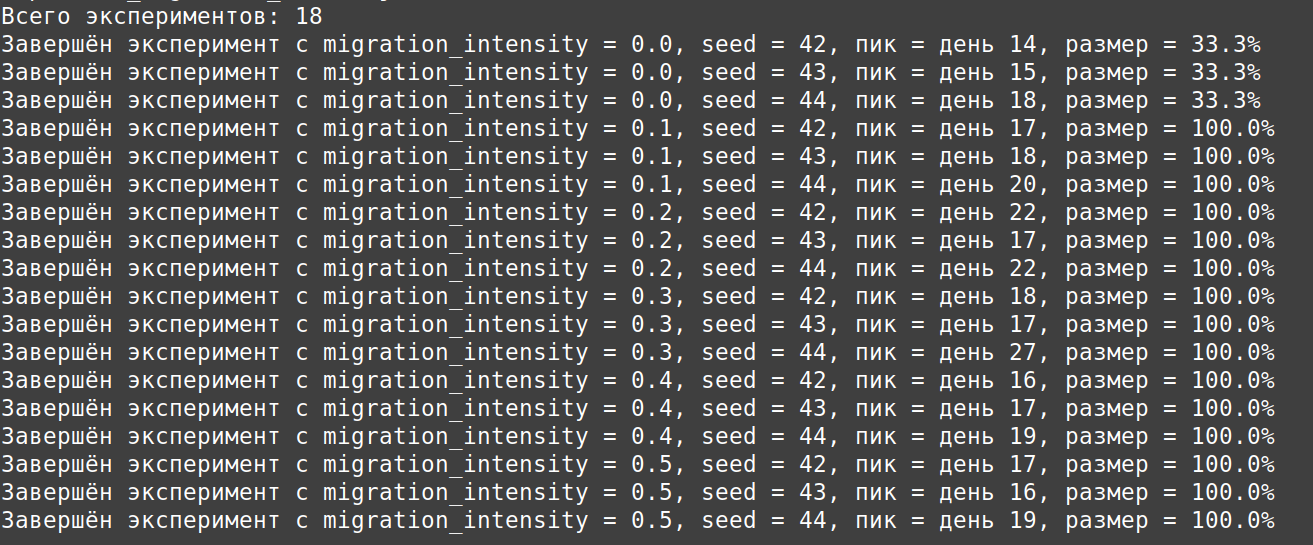
\includegraphics[width=0.7\textwidth,height=\textheight]{image/pic29.png}

}

\caption{\label{fig-026}интенсивности время до пика}

\end{figure}%

\section{5. Карантинные
меры}\label{ux43aux430ux440ux430ux43dux442ux438ux43dux43dux44bux435-ux43cux435ux440ux44b}

Я модифицирую модель, добавляя возможность закрытия города (сброса
миграции из него) при превышении порога заболеваемости(рис.27)

\begin{figure}

\centering{


\includegraphics[width=0.7\textwidth,height=\textheight]{image/pic30.png}

}

\caption{\label{fig-027}Карантинные меры}

\end{figure}%

Глядя на график, мы видим, что карантин в некоторых случаях немного
задерживает пик (до +13 дней), но не уменьшает его размер (по-прежнему
на 100\%)(рис.28)

\begin{figure}

\centering{


\includegraphics[width=0.7\textwidth,height=\textheight]{image/pic31.png}

}

\caption{\label{fig-028}Карантинные меры}

\end{figure}%

После этого я создала текст на основе литературного кода: чистого кода,
записной книжки jupyter и документации в формате Quarto. Я запускала все
ячейки в файле jupyter notebook, и все работает хорошо(рис.27)

\begin{figure}

\centering{

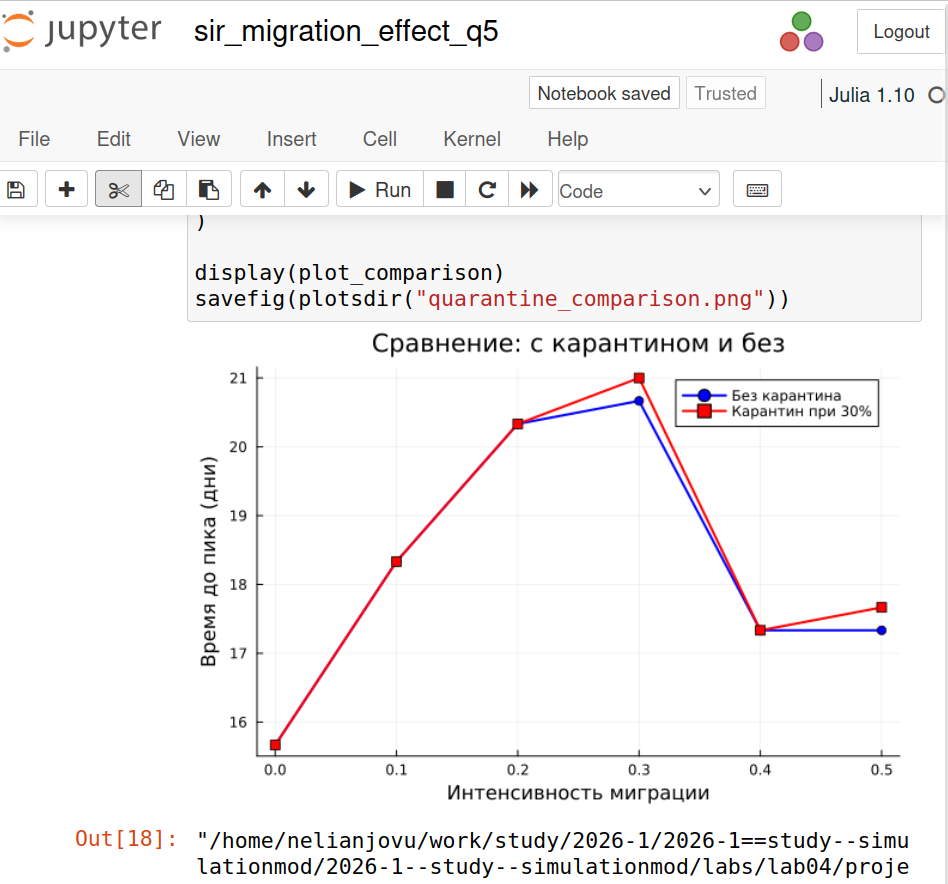
\includegraphics[width=0.7\textwidth,height=\textheight]{image/pic32.png}

}

\caption{\label{fig-027}создание файлов}

\end{figure}%

\textbf{\emph{Ниже приведен код, результаты расчетов и графики для кода
в файле scripts/sir\_migration\_effect\_q5.jl.qmd}}

\chapter{Исследование влияния миграции на динамику
эпидемии}\label{ux438ux441ux441ux43bux435ux434ux43eux432ux430ux43dux438ux435-ux432ux43bux438ux44fux43dux438ux44f-ux43cux438ux433ux440ux430ux446ux438ux438-ux43dux430-ux434ux438ux43dux430ux43cux438ux43aux443-ux44dux43fux438ux434ux435ux43cux438ux438-1}

\textbf{Цель:} Изучить, как интенсивность перемещения людей между
городами влияет на скорость распространения эпидемии (время достижения
пика) и масштаб пика. Инфекция начинается только в одном городе,
остальные изначально здоровы.

\section{Подготовка
окружения}\label{ux43fux43eux434ux433ux43eux442ux43eux432ux43aux430-ux43eux43aux440ux443ux436ux435ux43dux438ux44f-1}

\begin{Shaded}
\begin{Highlighting}[]
\ImportTok{using} \BuiltInTok{DrWatson}
\PreprocessorTok{@quickactivate} \StringTok{"project"}
\ImportTok{using} \BuiltInTok{Agents}\NormalTok{, }\BuiltInTok{DataFrames}\NormalTok{, }\BuiltInTok{Plots}\NormalTok{, }\BuiltInTok{CSV}\NormalTok{, }\BuiltInTok{Random}\NormalTok{, }\BuiltInTok{Statistics}

\FunctionTok{include}\NormalTok{(}\FunctionTok{srcdir}\NormalTok{(}\StringTok{"sir\_model.jl"}\NormalTok{))}
\end{Highlighting}
\end{Shaded}

\begin{verbatim}
┌ Warning: DrWatson could not find find a project file by recursively checking given `dir` and its parents. Returning `nothing` instead.
│ (given dir: /home/nelianjovu)
└ @ DrWatson ~/.julia/packages/DrWatson/2QF5p/src/project_setup.jl:84
\end{verbatim}

\begin{verbatim}
total_count (generic function with 1 method)
\end{verbatim}

\section{Функция для создания матрицы
миграции}\label{ux444ux443ux43dux43aux446ux438ux44f-ux434ux43bux44f-ux441ux43eux437ux434ux430ux43dux438ux44f-ux43cux430ux442ux440ux438ux446ux44b-ux43cux438ux433ux440ux430ux446ux438ux438-1}

Создаёт матрицу вероятностей миграции между городами на основе заданной
интенсивности. - \textbf{C}: количество городов - \textbf{intensity}:
вероятность миграции в другой город

Вероятность остаться в текущем городе: 1 - intensity Вероятность
переехать в конкретный другой город: intensity / (C-1)

\begin{Shaded}
\begin{Highlighting}[]
\KeywordTok{function} \FunctionTok{create\_migration\_matrix}\NormalTok{(C, intensity)}
\NormalTok{    M }\OperatorTok{=} \FunctionTok{ones}\NormalTok{(C, C) }\OperatorTok{.*}\NormalTok{ intensity }\OperatorTok{./}\NormalTok{ (C}\OperatorTok{{-}}\FloatTok{1}\NormalTok{)}
    \ControlFlowTok{for}\NormalTok{ i }\OperatorTok{=} \FloatTok{1}\OperatorTok{:}\NormalTok{C}
\NormalTok{        M[i, i] }\OperatorTok{=} \FloatTok{1} \OperatorTok{{-}}\NormalTok{ intensity}
    \ControlFlowTok{end}
    \ControlFlowTok{return}\NormalTok{ M}
\KeywordTok{end}
\end{Highlighting}
\end{Shaded}

\begin{verbatim}
create_migration_matrix (generic function with 1 method)
\end{verbatim}

\section{Функция для применения
карантина}\label{ux444ux443ux43dux43aux446ux438ux44f-ux434ux43bux44f-ux43fux440ux438ux43cux435ux43dux435ux43dux438ux44f-ux43aux430ux440ux430ux43dux442ux438ux43dux430}

Проверяет каждый город на превышение порога заболеваемости и закрывает
его при необходимости.

\begin{Shaded}
\begin{Highlighting}[]
\KeywordTok{function} \FunctionTok{apply\_quarantine!}\NormalTok{(model, quarantine\_active, threshold)}
    \ControlFlowTok{for}\NormalTok{ city\_id }\KeywordTok{in} \FloatTok{1}\OperatorTok{:}\NormalTok{model.C}
        \ControlFlowTok{if}\NormalTok{ quarantine\_active[city\_id]}\CommentTok{\# Если город уже на карантине, пропускаем}
            \ControlFlowTok{continue}
        \ControlFlowTok{end}

\NormalTok{        current\_pop }\OperatorTok{=} \FunctionTok{count}\NormalTok{(a.pos }\OperatorTok{==}\NormalTok{ city\_id }\ControlFlowTok{for}\NormalTok{ a }\KeywordTok{in} \FunctionTok{allagents}\NormalTok{(model))}\CommentTok{\# Считаем текущую заболеваемость в городе}
        \ControlFlowTok{if}\NormalTok{ current\_pop }\OperatorTok{==} \FloatTok{0}
            \ControlFlowTok{continue}
        \ControlFlowTok{end}

\NormalTok{        infected\_count }\OperatorTok{=} \FunctionTok{count}\NormalTok{(a.status }\OperatorTok{==} \OperatorTok{:}\NormalTok{I }\OperatorTok{\&\&}\NormalTok{ a.pos }\OperatorTok{==}\NormalTok{ city\_id }\ControlFlowTok{for}\NormalTok{ a }\KeywordTok{in} \FunctionTok{allagents}\NormalTok{(model))}
\NormalTok{        infected\_pct }\OperatorTok{=}\NormalTok{ infected\_count }\OperatorTok{/}\NormalTok{ current\_pop}

        \ControlFlowTok{if}\NormalTok{ infected\_pct }\OperatorTok{\textgreater{}}\NormalTok{ threshold}\CommentTok{\# Если порог превышен, закрываем город}
\NormalTok{            quarantine\_active[city\_id] }\OperatorTok{=} \ConstantTok{true}

\NormalTok{            model.migration\_rates[city\_id, }\OperatorTok{:}\NormalTok{] }\OperatorTok{.=} \FloatTok{0}\CommentTok{\# Обнуляем миграцию из города}
\NormalTok{            model.migration\_rates[}\OperatorTok{:}\NormalTok{, city\_id] }\OperatorTok{.=} \FloatTok{0}\CommentTok{\# Обнуляем миграцию в город}
\NormalTok{            model.migration\_rates[city\_id, city\_id] }\OperatorTok{=} \FloatTok{1.0}\CommentTok{\# Люди остаются на месте}

            \FunctionTok{println}\NormalTok{(}\StringTok{"Город }\SpecialCharTok{$}\NormalTok{city\_id}\StringTok{ ЗАКРЫТ на карантин! (заболеваемость: }\SpecialCharTok{$}\NormalTok{(}\FunctionTok{round}\NormalTok{(infected\_pct}\OperatorTok{*}\FloatTok{100}\NormalTok{, digits}\OperatorTok{=}\FloatTok{1}\NormalTok{))}\StringTok{\%)"}\NormalTok{)}
        \ControlFlowTok{end}
    \ControlFlowTok{end}
\ControlFlowTok{end}
\end{Highlighting}
\end{Shaded}

\begin{verbatim}
apply_quarantine! (generic function with 1 method)
\end{verbatim}

\section{Функция для измерения времени достижения
пика}\label{ux444ux443ux43dux43aux446ux438ux44f-ux434ux43bux44f-ux438ux437ux43cux435ux440ux435ux43dux438ux44f-ux432ux440ux435ux43cux435ux43dux438-ux434ux43eux441ux442ux438ux436ux435ux43dux438ux44f-ux43fux438ux43aux430-1}

Запускает симуляцию с заданной интенсивностью миграции и возвращает: -
\textbf{peak\_time}: день, когда доля инфицированных достигла максимума
- \textbf{peak\_value}: максимальная доля инфицированных

\begin{Shaded}
\begin{Highlighting}[]
\KeywordTok{function} \FunctionTok{peak\_time\_with\_quarantine}\NormalTok{(p)}
\NormalTok{    migration\_rates }\OperatorTok{=} \FunctionTok{create\_migration\_matrix}\NormalTok{(p[}\OperatorTok{:}\NormalTok{C], p[}\OperatorTok{:}\NormalTok{migration\_intensity])}\CommentTok{\# Создаём матрицу миграции на основе интенсивности}

\NormalTok{    model }\OperatorTok{=} \FunctionTok{initialize\_sir}\NormalTok{(;}
\NormalTok{        Ns }\OperatorTok{=}\NormalTok{ p[}\OperatorTok{:}\NormalTok{Ns],}
\NormalTok{        β\_und }\OperatorTok{=}\NormalTok{ p[}\OperatorTok{:}\NormalTok{β\_und],}
\NormalTok{        β\_det }\OperatorTok{=}\NormalTok{ p[}\OperatorTok{:}\NormalTok{β\_det],}
\NormalTok{        infection\_period }\OperatorTok{=}\NormalTok{ p[}\OperatorTok{:}\NormalTok{infection\_period],}
\NormalTok{        detection\_time }\OperatorTok{=}\NormalTok{ p[}\OperatorTok{:}\NormalTok{detection\_time],}
\NormalTok{        death\_rate }\OperatorTok{=}\NormalTok{ p[}\OperatorTok{:}\NormalTok{death\_rate],}
\NormalTok{        reinfection\_probability }\OperatorTok{=}\NormalTok{ p[}\OperatorTok{:}\NormalTok{reinfection\_probability],}
\NormalTok{        Is }\OperatorTok{=}\NormalTok{ p[}\OperatorTok{:}\NormalTok{Is],}
\NormalTok{        seed }\OperatorTok{=}\NormalTok{ p[}\OperatorTok{:}\NormalTok{seed],}
\NormalTok{        migration\_rates }\OperatorTok{=}\NormalTok{ migration\_rates,}
\NormalTok{    )}

\NormalTok{    quarantine\_active }\OperatorTok{=}\NormalTok{ [}\ConstantTok{false}\NormalTok{, }\ConstantTok{false}\NormalTok{, }\ConstantTok{false}\NormalTok{]}\CommentTok{\# Отслеживаем активный карантин для каждого города}

    \FunctionTok{infected\_frac}\NormalTok{(model) }\OperatorTok{=} \FunctionTok{count}\NormalTok{(a.status }\OperatorTok{==} \OperatorTok{:}\NormalTok{I }\ControlFlowTok{for}\NormalTok{ a }\KeywordTok{in} \FunctionTok{allagents}\NormalTok{(model)) }\OperatorTok{/} \FunctionTok{nagents}\NormalTok{(model)}
\NormalTok{    peak }\OperatorTok{=} \FloatTok{0.0}
\NormalTok{    peak\_step }\OperatorTok{=} \FloatTok{0}

    \ControlFlowTok{for}\NormalTok{ step }\OperatorTok{=} \FloatTok{1}\OperatorTok{:}\NormalTok{p[}\OperatorTok{:}\NormalTok{n\_steps]}
        \FunctionTok{apply\_quarantine!}\NormalTok{(model, quarantine\_active, p[}\OperatorTok{:}\NormalTok{quarantine\_threshold])}\CommentTok{\# Применяем карантин перед шагом агентов}
\NormalTok{        agent\_ids }\OperatorTok{=} \FunctionTok{collect}\NormalTok{(}\FunctionTok{allids}\NormalTok{(model))}
        \ControlFlowTok{for}\NormalTok{ id }\KeywordTok{in}\NormalTok{ agent\_ids}
\NormalTok{            agent }\OperatorTok{=} \ControlFlowTok{try}
\NormalTok{                model[id]}
            \ControlFlowTok{catch}
                \ConstantTok{nothing}
            \ControlFlowTok{end}
            \ControlFlowTok{if}\NormalTok{ agent }\OperatorTok{!==} \ConstantTok{nothing}
                \FunctionTok{sir\_agent\_step!}\NormalTok{(agent, model)}
            \ControlFlowTok{end}
        \ControlFlowTok{end}

\NormalTok{        frac }\OperatorTok{=} \FunctionTok{infected\_frac}\NormalTok{(model)}
        \ControlFlowTok{if}\NormalTok{ frac }\OperatorTok{\textgreater{}}\NormalTok{ peak}
\NormalTok{            peak }\OperatorTok{=}\NormalTok{ frac}
\NormalTok{            peak\_step }\OperatorTok{=}\NormalTok{ step}
        \ControlFlowTok{end}
    \ControlFlowTok{end}

    \ControlFlowTok{return}\NormalTok{ (peak\_time }\OperatorTok{=}\NormalTok{ peak\_step, peak\_value }\OperatorTok{=}\NormalTok{ peak)}
\KeywordTok{end}\CommentTok{\# Ручной пошаговый запуск симуляции}
\end{Highlighting}
\end{Shaded}

\begin{verbatim}
peak_time_with_quarantine (generic function with 1 method)
\end{verbatim}

\section{Функция для измерения времени достижения пика БЕЗ
карантина}\label{ux444ux443ux43dux43aux446ux438ux44f-ux434ux43bux44f-ux438ux437ux43cux435ux440ux435ux43dux438ux44f-ux432ux440ux435ux43cux435ux43dux438-ux434ux43eux441ux442ux438ux436ux435ux43dux438ux44f-ux43fux438ux43aux430-ux431ux435ux437-ux43aux430ux440ux430ux43dux442ux438ux43dux430}

Запускает симуляцию с заданной интенсивностью миграции без карантина.

\begin{Shaded}
\begin{Highlighting}[]
\KeywordTok{function} \FunctionTok{peak\_time\_no\_quarantine}\NormalTok{(p)}
\NormalTok{    migration\_rates }\OperatorTok{=} \FunctionTok{create\_migration\_matrix}\NormalTok{(p[}\OperatorTok{:}\NormalTok{C], p[}\OperatorTok{:}\NormalTok{migration\_intensity])}

\NormalTok{    model }\OperatorTok{=} \FunctionTok{initialize\_sir}\NormalTok{(;}
\NormalTok{        Ns }\OperatorTok{=}\NormalTok{ p[}\OperatorTok{:}\NormalTok{Ns],}
\NormalTok{        β\_und }\OperatorTok{=}\NormalTok{ p[}\OperatorTok{:}\NormalTok{β\_und],}
\NormalTok{        β\_det }\OperatorTok{=}\NormalTok{ p[}\OperatorTok{:}\NormalTok{β\_det],}
\NormalTok{        infection\_period }\OperatorTok{=}\NormalTok{ p[}\OperatorTok{:}\NormalTok{infection\_period],}
\NormalTok{        detection\_time }\OperatorTok{=}\NormalTok{ p[}\OperatorTok{:}\NormalTok{detection\_time],}
\NormalTok{        death\_rate }\OperatorTok{=}\NormalTok{ p[}\OperatorTok{:}\NormalTok{death\_rate],}
\NormalTok{        reinfection\_probability }\OperatorTok{=}\NormalTok{ p[}\OperatorTok{:}\NormalTok{reinfection\_probability],}
\NormalTok{        Is }\OperatorTok{=}\NormalTok{ p[}\OperatorTok{:}\NormalTok{Is],}
\NormalTok{        seed }\OperatorTok{=}\NormalTok{ p[}\OperatorTok{:}\NormalTok{seed],}
\NormalTok{        migration\_rates }\OperatorTok{=}\NormalTok{ migration\_rates,}
\NormalTok{    )}

    \FunctionTok{infected\_frac}\NormalTok{(model) }\OperatorTok{=} \FunctionTok{count}\NormalTok{(a.status }\OperatorTok{==} \OperatorTok{:}\NormalTok{I }\ControlFlowTok{for}\NormalTok{ a }\KeywordTok{in} \FunctionTok{allagents}\NormalTok{(model)) }\OperatorTok{/} \FunctionTok{nagents}\NormalTok{(model)}

\NormalTok{    peak }\OperatorTok{=} \FloatTok{0.0}
\NormalTok{    peak\_step }\OperatorTok{=} \FloatTok{0}

    \ControlFlowTok{for}\NormalTok{ step }\OperatorTok{=} \FloatTok{1}\OperatorTok{:}\NormalTok{p[}\OperatorTok{:}\NormalTok{n\_steps]}
\NormalTok{        agent\_ids }\OperatorTok{=} \FunctionTok{collect}\NormalTok{(}\FunctionTok{allids}\NormalTok{(model))}
        \ControlFlowTok{for}\NormalTok{ id }\KeywordTok{in}\NormalTok{ agent\_ids}
\NormalTok{            agent }\OperatorTok{=} \ControlFlowTok{try}
\NormalTok{                model[id]}
            \ControlFlowTok{catch}
                \ConstantTok{nothing}
            \ControlFlowTok{end}
            \ControlFlowTok{if}\NormalTok{ agent }\OperatorTok{!==} \ConstantTok{nothing}
                \FunctionTok{sir\_agent\_step!}\NormalTok{(agent, model)}
            \ControlFlowTok{end}
        \ControlFlowTok{end}

\NormalTok{        frac }\OperatorTok{=} \FunctionTok{infected\_frac}\NormalTok{(model)}
        \ControlFlowTok{if}\NormalTok{ frac }\OperatorTok{\textgreater{}}\NormalTok{ peak}
\NormalTok{            peak }\OperatorTok{=}\NormalTok{ frac}
\NormalTok{            peak\_step }\OperatorTok{=}\NormalTok{ step}
        \ControlFlowTok{end}
    \ControlFlowTok{end}

    \ControlFlowTok{return}\NormalTok{ (peak\_time }\OperatorTok{=}\NormalTok{ peak\_step, peak\_value }\OperatorTok{=}\NormalTok{ peak)}
\KeywordTok{end}
\end{Highlighting}
\end{Shaded}

\begin{verbatim}
peak_time_no_quarantine (generic function with 1 method)
\end{verbatim}

ЭКСПЕРИМЕНТ: СРАВНЕНИЕ С КАРАНТИНОМ И БЕЗ

\begin{Shaded}
\begin{Highlighting}[]
\FunctionTok{println}\NormalTok{(}\StringTok{"ЗАДАНИЕ 5: ИССЛЕДОВАНИЕ ЭФФЕКТИВНОСТИ КАРАНТИНА"}\NormalTok{)}
\end{Highlighting}
\end{Shaded}

\begin{verbatim}
ЗАДАНИЕ 5: ИССЛЕДОВАНИЕ ЭФФЕКТИВНОСТИ КАРАНТИНА
\end{verbatim}

Параметры эксперимента

\begin{Shaded}
\begin{Highlighting}[]
\NormalTok{base\_params }\OperatorTok{=} \FunctionTok{Dict}\NormalTok{(}
    \OperatorTok{:}\NormalTok{C }\OperatorTok{=\textgreater{}} \FloatTok{3}\NormalTok{,}
    \OperatorTok{:}\NormalTok{Ns }\OperatorTok{=\textgreater{}}\NormalTok{ [}\FloatTok{1000}\NormalTok{, }\FloatTok{1000}\NormalTok{, }\FloatTok{1000}\NormalTok{],}
    \OperatorTok{:}\NormalTok{β\_und }\OperatorTok{=\textgreater{}}\NormalTok{ [}\FloatTok{0.5}\NormalTok{, }\FloatTok{0.5}\NormalTok{, }\FloatTok{0.5}\NormalTok{],}
    \OperatorTok{:}\NormalTok{β\_det }\OperatorTok{=\textgreater{}}\NormalTok{ [}\FloatTok{0.05}\NormalTok{, }\FloatTok{0.05}\NormalTok{, }\FloatTok{0.05}\NormalTok{],}
    \OperatorTok{:}\NormalTok{infection\_period }\OperatorTok{=\textgreater{}} \FloatTok{14}\NormalTok{,}
    \OperatorTok{:}\NormalTok{detection\_time }\OperatorTok{=\textgreater{}} \FloatTok{7}\NormalTok{,}
    \OperatorTok{:}\NormalTok{death\_rate }\OperatorTok{=\textgreater{}} \FloatTok{0.02}\NormalTok{,}
    \OperatorTok{:}\NormalTok{reinfection\_probability }\OperatorTok{=\textgreater{}} \FloatTok{0.1}\NormalTok{,}
    \OperatorTok{:}\NormalTok{Is }\OperatorTok{=\textgreater{}}\NormalTok{ [}\FloatTok{1}\NormalTok{, }\FloatTok{0}\NormalTok{, }\FloatTok{0}\NormalTok{],}
    \OperatorTok{:}\NormalTok{n\_steps }\OperatorTok{=\textgreater{}} \FloatTok{150}\NormalTok{,}
\NormalTok{)}
\end{Highlighting}
\end{Shaded}

\begin{verbatim}
Dict{Symbol, Any} with 10 entries:
  :death_rate              => 0.02
  :Is                      => [1, 0, 0]
  :infection_period        => 14
  :n_steps                 => 150
  :β_und                   => [0.5, 0.5, 0.5]
  :Ns                      => [1000, 1000, 1000]
  :detection_time          => 7
  :reinfection_probability => 0.1
  :β_det                   => [0.05, 0.05, 0.05]
  :C                       => 3
\end{verbatim}

Тестируем разные интенсивности миграции

\begin{Shaded}
\begin{Highlighting}[]
\NormalTok{migration\_intensities }\OperatorTok{=}\NormalTok{ [}\FloatTok{0.0}\NormalTok{, }\FloatTok{0.1}\NormalTok{, }\FloatTok{0.2}\NormalTok{, }\FloatTok{0.3}\NormalTok{, }\FloatTok{0.4}\NormalTok{, }\FloatTok{0.5}\NormalTok{]}
\NormalTok{seeds }\OperatorTok{=}\NormalTok{ [}\FloatTok{42}\NormalTok{, }\FloatTok{43}\NormalTok{, }\FloatTok{44}\NormalTok{]}
\end{Highlighting}
\end{Shaded}

\begin{verbatim}
3-element Vector{Int64}:
 42
 43
 44
\end{verbatim}

Пороги карантина для тестирования

\begin{Shaded}
\begin{Highlighting}[]
\NormalTok{quarantine\_thresholds }\OperatorTok{=}\NormalTok{ [}\FloatTok{0.10}\NormalTok{, }\FloatTok{0.20}\NormalTok{, }\FloatTok{0.30}\NormalTok{, }\FloatTok{0.40}\NormalTok{]  }\CommentTok{\# 10\%, 20\%, 30\%, 40\%}

\NormalTok{results\_no\_quarantine }\OperatorTok{=}\NormalTok{ []}
\NormalTok{results\_with\_quarantine }\OperatorTok{=} \FunctionTok{Dict}\NormalTok{()}

\FunctionTok{println}\NormalTok{(}\StringTok{"}\SpecialCharTok{\textbackslash{}n}\StringTok{Запуск экспериментов БЕЗ карантина..."}\NormalTok{)}

\ControlFlowTok{for}\NormalTok{ mig }\KeywordTok{in}\NormalTok{ migration\_intensities}
    \ControlFlowTok{for}\NormalTok{ s }\KeywordTok{in}\NormalTok{ seeds}
\NormalTok{        params }\OperatorTok{=} \FunctionTok{merge}\NormalTok{(base\_params, }\FunctionTok{Dict}\NormalTok{(}
            \OperatorTok{:}\NormalTok{migration\_intensity }\OperatorTok{=\textgreater{}}\NormalTok{ mig,}
            \OperatorTok{:}\NormalTok{seed }\OperatorTok{=\textgreater{}}\NormalTok{ s,}
\NormalTok{        ))}
\NormalTok{        data }\OperatorTok{=} \FunctionTok{peak\_time\_no\_quarantine}\NormalTok{(params)}
        \FunctionTok{push!}\NormalTok{(results\_no\_quarantine, }\FunctionTok{merge}\NormalTok{(params, }\FunctionTok{Dict}\NormalTok{(}\FunctionTok{pairs}\NormalTok{(data))))}
        \FunctionTok{println}\NormalTok{(}\StringTok{"  БЕЗ карантина: mig = }\SpecialCharTok{$}\NormalTok{mig}\StringTok{, seed = }\SpecialCharTok{$}\NormalTok{s}\StringTok{, пик = день }\SpecialCharTok{$}\NormalTok{(data.peak\_time)}\StringTok{, размер = }\SpecialCharTok{$}\NormalTok{(}\FunctionTok{round}\NormalTok{(data.peak\_value }\OperatorTok{*} \FloatTok{100}\NormalTok{, digits}\OperatorTok{=}\FloatTok{1}\NormalTok{))}\StringTok{\%"}\NormalTok{)}
    \ControlFlowTok{end}
\ControlFlowTok{end}

\FunctionTok{println}\NormalTok{(}\StringTok{"}\SpecialCharTok{\textbackslash{}n}\StringTok{Запуск экспериментов С КАРАНТИНОМ..."}\NormalTok{)}

\ControlFlowTok{for}\NormalTok{ threshold }\KeywordTok{in}\NormalTok{ quarantine\_thresholds}
\NormalTok{    results\_with\_quarantine[threshold] }\OperatorTok{=}\NormalTok{ []}
    \ControlFlowTok{for}\NormalTok{ mig }\KeywordTok{in}\NormalTok{ migration\_intensities}
        \ControlFlowTok{for}\NormalTok{ s }\KeywordTok{in}\NormalTok{ seeds}
\NormalTok{            params }\OperatorTok{=} \FunctionTok{merge}\NormalTok{(base\_params, }\FunctionTok{Dict}\NormalTok{(}
                \OperatorTok{:}\NormalTok{migration\_intensity }\OperatorTok{=\textgreater{}}\NormalTok{ mig,}
                \OperatorTok{:}\NormalTok{seed }\OperatorTok{=\textgreater{}}\NormalTok{ s,}
                \OperatorTok{:}\NormalTok{quarantine\_threshold }\OperatorTok{=\textgreater{}}\NormalTok{ threshold,}
\NormalTok{            ))}
\NormalTok{            data }\OperatorTok{=} \FunctionTok{peak\_time\_with\_quarantine}\NormalTok{(params)}
            \FunctionTok{push!}\NormalTok{(results\_with\_quarantine[threshold], }\FunctionTok{merge}\NormalTok{(params, }\FunctionTok{Dict}\NormalTok{(}\FunctionTok{pairs}\NormalTok{(data))))}
            \FunctionTok{println}\NormalTok{(}\StringTok{"  С КАРАНТИНОМ (}\SpecialCharTok{$}\NormalTok{(}\FunctionTok{Int}\NormalTok{(threshold}\OperatorTok{*}\FloatTok{100}\NormalTok{))}\StringTok{\%): mig = }\SpecialCharTok{$}\NormalTok{mig}\StringTok{, seed = }\SpecialCharTok{$}\NormalTok{s}\StringTok{, пик = день }\SpecialCharTok{$}\NormalTok{(data.peak\_time)}\StringTok{, размер = }\SpecialCharTok{$}\NormalTok{(}\FunctionTok{round}\NormalTok{(data.peak\_value }\OperatorTok{*} \FloatTok{100}\NormalTok{, digits}\OperatorTok{=}\FloatTok{1}\NormalTok{))}\StringTok{\%"}\NormalTok{)}
        \ControlFlowTok{end}
    \ControlFlowTok{end}
\ControlFlowTok{end}
\end{Highlighting}
\end{Shaded}

\begin{verbatim}

Запуск экспериментов БЕЗ карантина...
  БЕЗ карантина: mig = 0.0, seed = 42, пик = день 14, размер = 33.3%
  БЕЗ карантина: mig = 0.0, seed = 43, пик = день 15, размер = 33.3%
  БЕЗ карантина: mig = 0.0, seed = 44, пик = день 18, размер = 33.3%
  БЕЗ карантина: mig = 0.1, seed = 42, пик = день 17, размер = 100.0%
  БЕЗ карантина: mig = 0.1, seed = 43, пик = день 18, размер = 100.0%
  БЕЗ карантина: mig = 0.1, seed = 44, пик = день 20, размер = 100.0%
  БЕЗ карантина: mig = 0.2, seed = 42, пик = день 22, размер = 100.0%
  БЕЗ карантина: mig = 0.2, seed = 43, пик = день 17, размер = 100.0%
  БЕЗ карантина: mig = 0.2, seed = 44, пик = день 22, размер = 100.0%
  БЕЗ карантина: mig = 0.3, seed = 42, пик = день 18, размер = 100.0%
  БЕЗ карантина: mig = 0.3, seed = 43, пик = день 17, размер = 100.0%
  БЕЗ карантина: mig = 0.3, seed = 44, пик = день 27, размер = 100.0%
  БЕЗ карантина: mig = 0.4, seed = 42, пик = день 16, размер = 100.0%
  БЕЗ карантина: mig = 0.4, seed = 43, пик = день 17, размер = 100.0%
  БЕЗ карантина: mig = 0.4, seed = 44, пик = день 19, размер = 100.0%
  БЕЗ карантина: mig = 0.5, seed = 42, пик = день 17, размер = 100.0%
  БЕЗ карантина: mig = 0.5, seed = 43, пик = день 16, размер = 100.0%
  БЕЗ карантина: mig = 0.5, seed = 44, пик = день 19, размер = 100.0%

Запуск экспериментов С КАРАНТИНОМ...
Город 1 ЗАКРЫТ на карантин! (заболеваемость: 11.3%)
  С КАРАНТИНОМ (10%): mig = 0.0, seed = 42, пик = день 14, размер = 33.3%
Город 1 ЗАКРЫТ на карантин! (заболеваемость: 10.6%)
  С КАРАНТИНОМ (10%): mig = 0.0, seed = 43, пик = день 15, размер = 33.3%
Город 1 ЗАКРЫТ на карантин! (заболеваемость: 12.3%)
  С КАРАНТИНОМ (10%): mig = 0.0, seed = 44, пик = день 18, размер = 33.3%
Город 1 ЗАКРЫТ на карантин! (заболеваемость: 15.2%)
Город 2 ЗАКРЫТ на карантин! (заболеваемость: 13.4%)
Город 3 ЗАКРЫТ на карантин! (заболеваемость: 11.9%)
  С КАРАНТИНОМ (10%): mig = 0.1, seed = 42, пик = день 17, размер = 100.0%
Город 1 ЗАКРЫТ на карантин! (заболеваемость: 14.1%)
Город 2 ЗАКРЫТ на карантин! (заболеваемость: 10.0%)
Город 3 ЗАКРЫТ на карантин! (заболеваемость: 13.6%)
  С КАРАНТИНОМ (10%): mig = 0.1, seed = 43, пик = день 20, размер = 100.0%
Город 1 ЗАКРЫТ на карантин! (заболеваемость: 13.0%)
Город 2 ЗАКРЫТ на карантин! (заболеваемость: 13.5%)
Город 3 ЗАКРЫТ на карантин! (заболеваемость: 11.5%)
  С КАРАНТИНОМ (10%): mig = 0.1, seed = 44, пик = день 20, размер = 100.0%
Город 1 ЗАКРЫТ на карантин! (заболеваемость: 12.4%)
Город 2 ЗАКРЫТ на карантин! (заболеваемость: 12.3%)
Город 3 ЗАКРЫТ на карантин! (заболеваемость: 18.3%)
  С КАРАНТИНОМ (10%): mig = 0.2, seed = 42, пик = день 35, размер = 100.0%
Город 1 ЗАКРЫТ на карантин! (заболеваемость: 11.2%)
Город 2 ЗАКРЫТ на карантин! (заболеваемость: 11.9%)
Город 3 ЗАКРЫТ на карантин! (заболеваемость: 13.8%)
  С КАРАНТИНОМ (10%): mig = 0.2, seed = 43, пик = день 17, размер = 100.0%
Город 1 ЗАКРЫТ на карантин! (заболеваемость: 13.0%)
Город 2 ЗАКРЫТ на карантин! (заболеваемость: 16.0%)
Город 3 ЗАКРЫТ на карантин! (заболеваемость: 12.7%)
  С КАРАНТИНОМ (10%): mig = 0.2, seed = 44, пик = день 22, размер = 100.0%
Город 2 ЗАКРЫТ на карантин! (заболеваемость: 10.0%)
Город 3 ЗАКРЫТ на карантин! (заболеваемость: 13.9%)
Город 1 ЗАКРЫТ на карантин! (заболеваемость: 13.9%)
  С КАРАНТИНОМ (10%): mig = 0.3, seed = 42, пик = день 18, размер = 100.0%
Город 1 ЗАКРЫТ на карантин! (заболеваемость: 11.6%)
Город 2 ЗАКРЫТ на карантин! (заболеваемость: 11.5%)
Город 3 ЗАКРЫТ на карантин! (заболеваемость: 14.5%)
  С КАРАНТИНОМ (10%): mig = 0.3, seed = 43, пик = день 18, размер = 100.0%
Город 1 ЗАКРЫТ на карантин! (заболеваемость: 12.0%)
Город 2 ЗАКРЫТ на карантин! (заболеваемость: 11.8%)
Город 3 ЗАКРЫТ на карантин! (заболеваемость: 11.4%)
  С КАРАНТИНОМ (10%): mig = 0.3, seed = 44, пик = день 27, размер = 100.0%
Город 1 ЗАКРЫТ на карантин! (заболеваемость: 12.2%)
Город 2 ЗАКРЫТ на карантин! (заболеваемость: 13.9%)
Город 3 ЗАКРЫТ на карантин! (заболеваемость: 10.1%)
  С КАРАНТИНОМ (10%): mig = 0.4, seed = 42, пик = день 16, размер = 100.0%
Город 1 ЗАКРЫТ на карантин! (заболеваемость: 13.4%)
Город 2 ЗАКРЫТ на карантин! (заболеваемость: 12.0%)
Город 3 ЗАКРЫТ на карантин! (заболеваемость: 12.4%)
  С КАРАНТИНОМ (10%): mig = 0.4, seed = 43, пик = день 17, размер = 100.0%
Город 1 ЗАКРЫТ на карантин! (заболеваемость: 10.4%)
Город 2 ЗАКРЫТ на карантин! (заболеваемость: 14.2%)
Город 3 ЗАКРЫТ на карантин! (заболеваемость: 11.7%)
  С КАРАНТИНОМ (10%): mig = 0.4, seed = 44, пик = день 19, размер = 100.0%
Город 3 ЗАКРЫТ на карантин! (заболеваемость: 10.4%)
Город 1 ЗАКРЫТ на карантин! (заболеваемость: 11.9%)
Город 2 ЗАКРЫТ на карантин! (заболеваемость: 12.1%)
  С КАРАНТИНОМ (10%): mig = 0.5, seed = 42, пик = день 17, размер = 100.0%
Город 1 ЗАКРЫТ на карантин! (заболеваемость: 12.2%)
Город 2 ЗАКРЫТ на карантин! (заболеваемость: 13.0%)
Город 3 ЗАКРЫТ на карантин! (заболеваемость: 13.4%)
  С КАРАНТИНОМ (10%): mig = 0.5, seed = 43, пик = день 16, размер = 100.0%
Город 3 ЗАКРЫТ на карантин! (заболеваемость: 10.0%)
Город 1 ЗАКРЫТ на карантин! (заболеваемость: 13.0%)
Город 2 ЗАКРЫТ на карантин! (заболеваемость: 14.4%)
  С КАРАНТИНОМ (10%): mig = 0.5, seed = 44, пик = день 22, размер = 100.0%
Город 1 ЗАКРЫТ на карантин! (заболеваемость: 28.9%)
  С КАРАНТИНОМ (20%): mig = 0.0, seed = 42, пик = день 14, размер = 33.3%
Город 1 ЗАКРЫТ на карантин! (заболеваемость: 27.7%)
  С КАРАНТИНОМ (20%): mig = 0.0, seed = 43, пик = день 15, размер = 33.3%
Город 1 ЗАКРЫТ на карантин! (заболеваемость: 30.8%)
  С КАРАНТИНОМ (20%): mig = 0.0, seed = 44, пик = день 18, размер = 33.3%
Город 1 ЗАКРЫТ на карантин! (заболеваемость: 22.3%)
Город 2 ЗАКРЫТ на карантин! (заболеваемость: 22.0%)
Город 3 ЗАКРЫТ на карантин! (заболеваемость: 31.2%)
  С КАРАНТИНОМ (20%): mig = 0.1, seed = 42, пик = день 17, размер = 100.0%
Город 1 ЗАКРЫТ на карантин! (заболеваемость: 20.7%)
Город 2 ЗАКРЫТ на карантин! (заболеваемость: 26.3%)
Город 3 ЗАКРЫТ на карантин! (заболеваемость: 23.5%)
  С КАРАНТИНОМ (20%): mig = 0.1, seed = 43, пик = день 19, размер = 100.0%
Город 1 ЗАКРЫТ на карантин! (заболеваемость: 31.0%)
Город 2 ЗАКРЫТ на карантин! (заболеваемость: 23.5%)
Город 3 ЗАКРЫТ на карантин! (заболеваемость: 28.7%)
  С КАРАНТИНОМ (20%): mig = 0.1, seed = 44, пик = день 20, размер = 100.0%
Город 1 ЗАКРЫТ на карантин! (заболеваемость: 27.5%)
Город 2 ЗАКРЫТ на карантин! (заболеваемость: 29.8%)
Город 3 ЗАКРЫТ на карантин! (заболеваемость: 28.9%)
  С КАРАНТИНОМ (20%): mig = 0.2, seed = 42, пик = день 22, размер = 100.0%
Город 3 ЗАКРЫТ на карантин! (заболеваемость: 20.3%)
Город 1 ЗАКРЫТ на карантин! (заболеваемость: 29.3%)
Город 2 ЗАКРЫТ на карантин! (заболеваемость: 28.6%)
  С КАРАНТИНОМ (20%): mig = 0.2, seed = 43, пик = день 17, размер = 100.0%
Город 1 ЗАКРЫТ на карантин! (заболеваемость: 21.2%)
Город 2 ЗАКРЫТ на карантин! (заболеваемость: 25.9%)
Город 3 ЗАКРЫТ на карантин! (заболеваемость: 21.0%)
  С КАРАНТИНОМ (20%): mig = 0.2, seed = 44, пик = день 22, размер = 100.0%
Город 1 ЗАКРЫТ на карантин! (заболеваемость: 20.9%)
Город 2 ЗАКРЫТ на карантин! (заболеваемость: 28.5%)
Город 3 ЗАКРЫТ на карантин! (заболеваемость: 27.7%)
  С КАРАНТИНОМ (20%): mig = 0.3, seed = 42, пик = день 18, размер = 100.0%
Город 1 ЗАКРЫТ на карантин! (заболеваемость: 31.7%)
Город 2 ЗАКРЫТ на карантин! (заболеваемость: 26.0%)
Город 3 ЗАКРЫТ на карантин! (заболеваемость: 28.8%)
  С КАРАНТИНОМ (20%): mig = 0.3, seed = 43, пик = день 17, размер = 100.0%
Город 1 ЗАКРЫТ на карантин! (заболеваемость: 29.0%)
Город 2 ЗАКРЫТ на карантин! (заболеваемость: 31.9%)
Город 3 ЗАКРЫТ на карантин! (заболеваемость: 32.8%)
  С КАРАНТИНОМ (20%): mig = 0.3, seed = 44, пик = день 27, размер = 100.0%
Город 1 ЗАКРЫТ на карантин! (заболеваемость: 31.1%)
Город 2 ЗАКРЫТ на карантин! (заболеваемость: 33.6%)
Город 3 ЗАКРЫТ на карантин! (заболеваемость: 29.6%)
  С КАРАНТИНОМ (20%): mig = 0.4, seed = 42, пик = день 16, размер = 100.0%
Город 1 ЗАКРЫТ на карантин! (заболеваемость: 21.1%)
Город 2 ЗАКРЫТ на карантин! (заболеваемость: 20.1%)
Город 3 ЗАКРЫТ на карантин! (заболеваемость: 20.5%)
  С КАРАНТИНОМ (20%): mig = 0.4, seed = 43, пик = день 17, размер = 100.0%
Город 1 ЗАКРЫТ на карантин! (заболеваемость: 20.6%)
Город 2 ЗАКРЫТ на карантин! (заболеваемость: 20.1%)
Город 3 ЗАКРЫТ на карантин! (заболеваемость: 26.0%)
  С КАРАНТИНОМ (20%): mig = 0.4, seed = 44, пик = день 19, размер = 100.0%
Город 1 ЗАКРЫТ на карантин! (заболеваемость: 20.1%)
Город 2 ЗАКРЫТ на карантин! (заболеваемость: 31.5%)
Город 3 ЗАКРЫТ на карантин! (заболеваемость: 32.7%)
  С КАРАНТИНОМ (20%): mig = 0.5, seed = 42, пик = день 17, размер = 100.0%
Город 1 ЗАКРЫТ на карантин! (заболеваемость: 21.0%)
Город 3 ЗАКРЫТ на карантин! (заболеваемость: 22.1%)
Город 2 ЗАКРЫТ на карантин! (заболеваемость: 36.3%)
  С КАРАНТИНОМ (20%): mig = 0.5, seed = 43, пик = день 16, размер = 100.0%
Город 1 ЗАКРЫТ на карантин! (заболеваемость: 22.3%)
Город 2 ЗАКРЫТ на карантин! (заболеваемость: 26.7%)
Город 3 ЗАКРЫТ на карантин! (заболеваемость: 27.0%)
  С КАРАНТИНОМ (20%): mig = 0.5, seed = 44, пик = день 21, размер = 100.0%
Город 1 ЗАКРЫТ на карантин! (заболеваемость: 47.3%)
  С КАРАНТИНОМ (30%): mig = 0.0, seed = 42, пик = день 14, размер = 33.3%
Город 1 ЗАКРЫТ на карантин! (заболеваемость: 43.2%)
  С КАРАНТИНОМ (30%): mig = 0.0, seed = 43, пик = день 15, размер = 33.3%
Город 1 ЗАКРЫТ на карантин! (заболеваемость: 30.8%)
  С КАРАНТИНОМ (30%): mig = 0.0, seed = 44, пик = день 18, размер = 33.3%
Город 1 ЗАКРЫТ на карантин! (заболеваемость: 35.4%)
Город 2 ЗАКРЫТ на карантин! (заболеваемость: 32.3%)
Город 3 ЗАКРЫТ на карантин! (заболеваемость: 42.8%)
  С КАРАНТИНОМ (30%): mig = 0.1, seed = 42, пик = день 17, размер = 100.0%
Город 1 ЗАКРЫТ на карантин! (заболеваемость: 32.5%)
Город 2 ЗАКРЫТ на карантин! (заболеваемость: 46.1%)
Город 3 ЗАКРЫТ на карантин! (заболеваемость: 40.2%)
  С КАРАНТИНОМ (30%): mig = 0.1, seed = 43, пик = день 18, размер = 100.0%
Город 1 ЗАКРЫТ на карантин! (заболеваемость: 31.0%)
Город 2 ЗАКРЫТ на карантин! (заболеваемость: 35.9%)
Город 3 ЗАКРЫТ на карантин! (заболеваемость: 45.8%)
  С КАРАНТИНОМ (30%): mig = 0.1, seed = 44, пик = день 20, размер = 100.0%
Город 1 ЗАКРЫТ на карантин! (заболеваемость: 50.1%)
Город 2 ЗАКРЫТ на карантин! (заболеваемость: 47.2%)
Город 3 ЗАКРЫТ на карантин! (заболеваемость: 47.8%)
  С КАРАНТИНОМ (30%): mig = 0.2, seed = 42, пик = день 22, размер = 100.0%
Город 1 ЗАКРЫТ на карантин! (заболеваемость: 31.3%)
Город 2 ЗАКРЫТ на карантин! (заболеваемость: 47.7%)
Город 3 ЗАКРЫТ на карантин! (заболеваемость: 45.9%)
  С КАРАНТИНОМ (30%): mig = 0.2, seed = 43, пик = день 17, размер = 100.0%
Город 1 ЗАКРЫТ на карантин! (заболеваемость: 34.8%)
Город 2 ЗАКРЫТ на карантин! (заболеваемость: 39.5%)
Город 3 ЗАКРЫТ на карантин! (заболеваемость: 32.1%)
  С КАРАНТИНОМ (30%): mig = 0.2, seed = 44, пик = день 22, размер = 100.0%
Город 1 ЗАКРЫТ на карантин! (заболеваемость: 31.2%)
Город 2 ЗАКРЫТ на карантин! (заболеваемость: 31.2%)
Город 3 ЗАКРЫТ на карантин! (заболеваемость: 30.6%)
  С КАРАНТИНОМ (30%): mig = 0.3, seed = 42, пик = день 19, размер = 100.0%
Город 1 ЗАКРЫТ на карантин! (заболеваемость: 31.7%)
Город 2 ЗАКРЫТ на карантин! (заболеваемость: 41.5%)
Город 3 ЗАКРЫТ на карантин! (заболеваемость: 46.8%)
  С КАРАНТИНОМ (30%): mig = 0.3, seed = 43, пик = день 17, размер = 100.0%
Город 2 ЗАКРЫТ на карантин! (заболеваемость: 31.9%)
Город 3 ЗАКРЫТ на карантин! (заболеваемость: 32.8%)
Город 1 ЗАКРЫТ на карантин! (заболеваемость: 47.0%)
  С КАРАНТИНОМ (30%): mig = 0.3, seed = 44, пик = день 27, размер = 100.0%
Город 1 ЗАКРЫТ на карантин! (заболеваемость: 31.1%)
Город 2 ЗАКРЫТ на карантин! (заболеваемость: 33.6%)
Город 3 ЗАКРЫТ на карантин! (заболеваемость: 47.8%)
  С КАРАНТИНОМ (30%): mig = 0.4, seed = 42, пик = день 16, размер = 100.0%
Город 1 ЗАКРЫТ на карантин! (заболеваемость: 35.0%)
Город 2 ЗАКРЫТ на карантин! (заболеваемость: 31.1%)
Город 3 ЗАКРЫТ на карантин! (заболеваемость: 32.9%)
  С КАРАНТИНОМ (30%): mig = 0.4, seed = 43, пик = день 17, размер = 100.0%
Город 1 ЗАКРЫТ на карантин! (заболеваемость: 33.7%)
Город 2 ЗАКРЫТ на карантин! (заболеваемость: 32.5%)
Город 3 ЗАКРЫТ на карантин! (заболеваемость: 45.7%)
  С КАРАНТИНОМ (30%): mig = 0.4, seed = 44, пик = день 19, размер = 100.0%
Город 1 ЗАКРЫТ на карантин! (заболеваемость: 30.6%)
Город 2 ЗАКРЫТ на карантин! (заболеваемость: 34.8%)
Город 3 ЗАКРЫТ на карантин! (заболеваемость: 48.0%)
  С КАРАНТИНОМ (30%): mig = 0.5, seed = 42, пик = день 17, размер = 100.0%
Город 1 ЗАКРЫТ на карантин! (заболеваемость: 32.3%)
Город 3 ЗАКРЫТ на карантин! (заболеваемость: 35.0%)
Город 2 ЗАКРЫТ на карантин! (заболеваемость: 49.3%)
  С КАРАНТИНОМ (30%): mig = 0.5, seed = 43, пик = день 16, размер = 100.0%
Город 1 ЗАКРЫТ на карантин! (заболеваемость: 44.8%)
Город 2 ЗАКРЫТ на карантин! (заболеваемость: 40.5%)
Город 3 ЗАКРЫТ на карантин! (заболеваемость: 38.7%)
  С КАРАНТИНОМ (30%): mig = 0.5, seed = 44, пик = день 20, размер = 100.0%
Город 1 ЗАКРЫТ на карантин! (заболеваемость: 47.3%)
  С КАРАНТИНОМ (40%): mig = 0.0, seed = 42, пик = день 14, размер = 33.3%
Город 1 ЗАКРЫТ на карантин! (заболеваемость: 43.2%)
  С КАРАНТИНОМ (40%): mig = 0.0, seed = 43, пик = день 15, размер = 33.3%
Город 1 ЗАКРЫТ на карантин! (заболеваемость: 47.1%)
  С КАРАНТИНОМ (40%): mig = 0.0, seed = 44, пик = день 18, размер = 33.3%
Город 1 ЗАКРЫТ на карантин! (заболеваемость: 56.7%)
Город 2 ЗАКРЫТ на карантин! (заболеваемость: 52.6%)
Город 3 ЗАКРЫТ на карантин! (заболеваемость: 46.9%)
  С КАРАНТИНОМ (40%): mig = 0.1, seed = 42, пик = день 17, размер = 100.0%
Город 1 ЗАКРЫТ на карантин! (заболеваемость: 49.6%)
Город 2 ЗАКРЫТ на карантин! (заболеваемость: 45.1%)
Город 3 ЗАКРЫТ на карантин! (заболеваемость: 40.8%)
  С КАРАНТИНОМ (40%): mig = 0.1, seed = 43, пик = день 18, размер = 100.0%
Город 1 ЗАКРЫТ на карантин! (заболеваемость: 47.5%)
Город 2 ЗАКРЫТ на карантин! (заболеваемость: 65.8%)
Город 3 ЗАКРЫТ на карантин! (заболеваемость: 51.8%)
  С КАРАНТИНОМ (40%): mig = 0.1, seed = 44, пик = день 20, размер = 100.0%
Город 1 ЗАКРЫТ на карантин! (заболеваемость: 50.1%)
Город 2 ЗАКРЫТ на карантин! (заболеваемость: 47.2%)
Город 3 ЗАКРЫТ на карантин! (заболеваемость: 47.8%)
  С КАРАНТИНОМ (40%): mig = 0.2, seed = 42, пик = день 22, размер = 100.0%
Город 1 ЗАКРЫТ на карантин! (заболеваемость: 44.1%)
Город 2 ЗАКРЫТ на карантин! (заболеваемость: 47.0%)
Город 3 ЗАКРЫТ на карантин! (заболеваемость: 46.2%)
  С КАРАНТИНОМ (40%): mig = 0.2, seed = 43, пик = день 17, размер = 100.0%
Город 1 ЗАКРЫТ на карантин! (заболеваемость: 56.3%)
Город 2 ЗАКРЫТ на карантин! (заболеваемость: 60.5%)
Город 3 ЗАКРЫТ на карантин! (заболеваемость: 59.7%)
  С КАРАНТИНОМ (40%): mig = 0.2, seed = 44, пик = день 22, размер = 100.0%
Город 1 ЗАКРЫТ на карантин! (заболеваемость: 50.1%)
Город 2 ЗАКРЫТ на карантин! (заболеваемость: 52.3%)
Город 3 ЗАКРЫТ на карантин! (заболеваемость: 48.8%)
  С КАРАНТИНОМ (40%): mig = 0.3, seed = 42, пик = день 19, размер = 100.0%
Город 1 ЗАКРЫТ на карантин! (заболеваемость: 48.7%)
Город 2 ЗАКРЫТ на карантин! (заболеваемость: 40.2%)
Город 3 ЗАКРЫТ на карантин! (заболеваемость: 47.7%)
  С КАРАНТИНОМ (40%): mig = 0.3, seed = 43, пик = день 18, размер = 100.0%
Город 1 ЗАКРЫТ на карантин! (заболеваемость: 48.4%)
Город 2 ЗАКРЫТ на карантин! (заболеваемость: 49.8%)
Город 3 ЗАКРЫТ на карантин! (заболеваемость: 50.3%)
  С КАРАНТИНОМ (40%): mig = 0.3, seed = 44, пик = день 27, размер = 100.0%
Город 1 ЗАКРЫТ на карантин! (заболеваемость: 51.6%)
Город 2 ЗАКРЫТ на карантин! (заболеваемость: 48.3%)
Город 3 ЗАКРЫТ на карантин! (заболеваемость: 49.5%)
  С КАРАНТИНОМ (40%): mig = 0.4, seed = 42, пик = день 16, размер = 100.0%
Город 1 ЗАКРЫТ на карантин! (заболеваемость: 50.3%)
Город 2 ЗАКРЫТ на карантин! (заболеваемость: 48.8%)
Город 3 ЗАКРЫТ на карантин! (заболеваемость: 53.8%)
  С КАРАНТИНОМ (40%): mig = 0.4, seed = 43, пик = день 17, размер = 100.0%
Город 1 ЗАКРЫТ на карантин! (заболеваемость: 50.8%)
Город 2 ЗАКРЫТ на карантин! (заболеваемость: 53.5%)
Город 3 ЗАКРЫТ на карантин! (заболеваемость: 53.0%)
  С КАРАНТИНОМ (40%): mig = 0.4, seed = 44, пик = день 19, размер = 100.0%
Город 1 ЗАКРЫТ на карантин! (заболеваемость: 52.5%)
Город 2 ЗАКРЫТ на карантин! (заболеваемость: 51.8%)
Город 3 ЗАКРЫТ на карантин! (заболеваемость: 50.1%)
  С КАРАНТИНОМ (40%): mig = 0.5, seed = 42, пик = день 17, размер = 100.0%
Город 1 ЗАКРЫТ на карантин! (заболеваемость: 53.2%)
Город 2 ЗАКРЫТ на карантин! (заболеваемость: 51.8%)
Город 3 ЗАКРЫТ на карантин! (заболеваемость: 54.7%)
  С КАРАНТИНОМ (40%): mig = 0.5, seed = 43, пик = день 16, размер = 100.0%
Город 1 ЗАКРЫТ на карантин! (заболеваемость: 44.8%)
Город 2 ЗАКРЫТ на карантин! (заболеваемость: 40.5%)
Город 3 ЗАКРЫТ на карантин! (заболеваемость: 61.7%)
  С КАРАНТИНОМ (40%): mig = 0.5, seed = 44, пик = день 20, размер = 100.0%
\end{verbatim}

РЕЗУЛЬТАТ

Усреднение результатов без карантина

\begin{Shaded}
\begin{Highlighting}[]
\NormalTok{df\_no\_quarantine }\OperatorTok{=} \FunctionTok{DataFrame}\NormalTok{(results\_no\_quarantine)}
\NormalTok{grouped\_no\_quarantine }\OperatorTok{=} \FunctionTok{combine}\NormalTok{(}
    \FunctionTok{groupby}\NormalTok{(df\_no\_quarantine, [}\OperatorTok{:}\NormalTok{migration\_intensity]),}
    \OperatorTok{:}\NormalTok{peak\_time }\OperatorTok{=\textgreater{}}\NormalTok{ mean }\OperatorTok{=\textgreater{}} \OperatorTok{:}\NormalTok{mean\_peak\_time,}
    \OperatorTok{:}\NormalTok{peak\_time }\OperatorTok{=\textgreater{}}\NormalTok{ std }\OperatorTok{=\textgreater{}} \OperatorTok{:}\NormalTok{std\_peak\_time,}
    \OperatorTok{:}\NormalTok{peak\_value }\OperatorTok{=\textgreater{}}\NormalTok{ mean }\OperatorTok{=\textgreater{}} \OperatorTok{:}\NormalTok{mean\_peak\_value,}
    \OperatorTok{:}\NormalTok{peak\_value }\OperatorTok{=\textgreater{}}\NormalTok{ std }\OperatorTok{=\textgreater{}} \OperatorTok{:}\NormalTok{std\_peak\_value,}
\NormalTok{)}
\end{Highlighting}
\end{Shaded}

\begin{tabular}{r|ccccc}
    & migration\_intensity & mean\_peak\_time & std\_peak\_time & mean\_peak\_value & std\_peak\_value\\
    \hline
    & Float64 & Float64 & Float64 & Float64 & Float64\\
    \hline
    1 & 0.0 & 15.6667 & 2.08167 & 0.333333 & 0.0 \\
    2 & 0.1 & 18.3333 & 1.52753 & 1.0 & 0.0 \\
    3 & 0.2 & 20.3333 & 2.88675 & 1.0 & 0.0 \\
    4 & 0.3 & 20.6667 & 5.50757 & 1.0 & 0.0 \\
    5 & 0.4 & 17.3333 & 1.52753 & 1.0 & 0.0 \\
    6 & 0.5 & 17.3333 & 1.52753 & 1.0 & 0.0 \\
\end{tabular}

Усреднение результатов с карантином для каждого порога

\begin{Shaded}
\begin{Highlighting}[]
\NormalTok{grouped\_with\_quarantine }\OperatorTok{=} \FunctionTok{Dict}\NormalTok{()}
\ControlFlowTok{for}\NormalTok{ threshold }\KeywordTok{in}\NormalTok{ quarantine\_thresholds}
\NormalTok{    df\_temp }\OperatorTok{=} \FunctionTok{DataFrame}\NormalTok{(results\_with\_quarantine[threshold])}
\NormalTok{    grouped\_with\_quarantine[threshold] }\OperatorTok{=} \FunctionTok{combine}\NormalTok{(}
        \FunctionTok{groupby}\NormalTok{(df\_temp, [}\OperatorTok{:}\NormalTok{migration\_intensity]),}
        \OperatorTok{:}\NormalTok{peak\_time }\OperatorTok{=\textgreater{}}\NormalTok{ mean }\OperatorTok{=\textgreater{}} \OperatorTok{:}\NormalTok{mean\_peak\_time,}
        \OperatorTok{:}\NormalTok{peak\_time }\OperatorTok{=\textgreater{}}\NormalTok{ std }\OperatorTok{=\textgreater{}} \OperatorTok{:}\NormalTok{std\_peak\_time,}
        \OperatorTok{:}\NormalTok{peak\_value }\OperatorTok{=\textgreater{}}\NormalTok{ mean }\OperatorTok{=\textgreater{}} \OperatorTok{:}\NormalTok{mean\_peak\_value,}
        \OperatorTok{:}\NormalTok{peak\_value }\OperatorTok{=\textgreater{}}\NormalTok{ std }\OperatorTok{=\textgreater{}} \OperatorTok{:}\NormalTok{std\_peak\_value,}
\NormalTok{    )}
\ControlFlowTok{end}
\end{Highlighting}
\end{Shaded}

ВИЗУАЛИЗАЦИЯ График 1: Сравнение времени пика (фиксированная миграция
0.3)

\begin{Shaded}
\begin{Highlighting}[]
\NormalTok{fixed\_mig }\OperatorTok{=} \FloatTok{0.3}
\end{Highlighting}
\end{Shaded}

\begin{verbatim}
0.3
\end{verbatim}

Находим данные для миграции 0.3 без карантина

\begin{Shaded}
\begin{Highlighting}[]
\NormalTok{row\_no }\OperatorTok{=}\NormalTok{ grouped\_no\_quarantine[}\FunctionTok{findfirst}\NormalTok{(}\OperatorTok{==}\NormalTok{(fixed\_mig), grouped\_no\_quarantine.migration\_intensity), }\OperatorTok{:}\NormalTok{]}
\end{Highlighting}
\end{Shaded}

\begin{tabular}{r|ccccc}
    & migration\_intensity & mean\_peak\_time & std\_peak\_time & mean\_peak\_value & std\_peak\_value\\
    \hline
    & Float64 & Float64 & Float64 & Float64 & Float64\\
    \hline
    4 & 0.3 & 20.6667 & 5.50757 & 1.0 & 0.0 \\
\end{tabular}

Собираем данные для миграции 0.3 с разными порогами карантина

\begin{Shaded}
\begin{Highlighting}[]
\NormalTok{peak\_times }\OperatorTok{=} \DataTypeTok{Float64}\NormalTok{[]}
\NormalTok{peak\_sizes }\OperatorTok{=} \DataTypeTok{Float64}\NormalTok{[]}
\NormalTok{threshold\_labels }\OperatorTok{=}\NormalTok{ [}\StringTok{"Без карантина"}\NormalTok{]}

\FunctionTok{push!}\NormalTok{(peak\_times, row\_no.mean\_peak\_time)}
\FunctionTok{push!}\NormalTok{(peak\_sizes, row\_no.mean\_peak\_value }\OperatorTok{*} \FloatTok{100}\NormalTok{)}

\ControlFlowTok{for}\NormalTok{ threshold }\KeywordTok{in}\NormalTok{ quarantine\_thresholds}
\NormalTok{    row }\OperatorTok{=}\NormalTok{ grouped\_with\_quarantine[threshold][}\FunctionTok{findfirst}\NormalTok{(}\OperatorTok{==}\NormalTok{(fixed\_mig), grouped\_with\_quarantine[threshold].migration\_intensity), }\OperatorTok{:}\NormalTok{]}
    \FunctionTok{push!}\NormalTok{(peak\_times, row.mean\_peak\_time)}
    \FunctionTok{push!}\NormalTok{(peak\_sizes, row.mean\_peak\_value }\OperatorTok{*} \FloatTok{100}\NormalTok{)}
    \FunctionTok{push!}\NormalTok{(threshold\_labels, }\StringTok{"}\SpecialCharTok{$}\NormalTok{(}\FunctionTok{Int}\NormalTok{(threshold}\OperatorTok{*}\FloatTok{100}\NormalTok{))}\StringTok{\% карантин"}\NormalTok{)}
\ControlFlowTok{end}
\end{Highlighting}
\end{Shaded}

График времени пика

\begin{Shaded}
\begin{Highlighting}[]
\NormalTok{plot\_peak\_time }\OperatorTok{=} \FunctionTok{bar}\NormalTok{(}
\NormalTok{    threshold\_labels,}
\NormalTok{    peak\_times,}
\NormalTok{    title }\OperatorTok{=} \StringTok{"Влияние карантина на время пика (миграция = }\SpecialCharTok{$}\NormalTok{fixed\_mig}\StringTok{)"}\NormalTok{,}
\NormalTok{    xlabel }\OperatorTok{=} \StringTok{"Сценарий"}\NormalTok{,}
\NormalTok{    ylabel }\OperatorTok{=} \StringTok{"Время до пика (дни)"}\NormalTok{,}
\NormalTok{    color }\OperatorTok{=} \OperatorTok{:}\NormalTok{steelblue,}
\NormalTok{    legend }\OperatorTok{=} \ConstantTok{false}\NormalTok{,}
\NormalTok{    grid }\OperatorTok{=} \ConstantTok{true}\NormalTok{,}
\NormalTok{)}

\FunctionTok{display}\NormalTok{(plot\_peak\_time)}
\FunctionTok{savefig}\NormalTok{(}\FunctionTok{plotsdir}\NormalTok{(}\StringTok{"quarantine\_peak\_time.png"}\NormalTok{))}
\end{Highlighting}
\end{Shaded}

\includesvg{simmod-lab04-report (Нджову Нелиа)_files/figure-pdf/cell-81-output-1.svg}

\includesvg{simmod-lab04-report (Нджову Нелиа)_files/figure-pdf/cell-81-output-2.svg}

\begin{verbatim}
"/home/nelianjovu/work/study/2026-1/2026-1==study--simulationmod/2026-1--study--simulationmod/labs/lab04/project/plots/quarantine_peak_time.png"
\end{verbatim}

График размера пика

\begin{Shaded}
\begin{Highlighting}[]
\NormalTok{plot\_peak\_size }\OperatorTok{=} \FunctionTok{bar}\NormalTok{(}
\NormalTok{    threshold\_labels,}
\NormalTok{    peak\_sizes,}
\NormalTok{    title }\OperatorTok{=} \StringTok{"Влияние карантина на размер пика (миграция = }\SpecialCharTok{$}\NormalTok{fixed\_mig}\StringTok{)"}\NormalTok{,}
\NormalTok{    xlabel }\OperatorTok{=} \StringTok{"Сценарий"}\NormalTok{,}
\NormalTok{    ylabel }\OperatorTok{=} \StringTok{"Размер пика (\% населения)"}\NormalTok{,}
\NormalTok{    color }\OperatorTok{=} \OperatorTok{:}\NormalTok{coral,}
\NormalTok{    legend }\OperatorTok{=} \ConstantTok{false}\NormalTok{,}
\NormalTok{    grid }\OperatorTok{=} \ConstantTok{true}\NormalTok{,}
\NormalTok{)}

\FunctionTok{display}\NormalTok{(plot\_peak\_size)}
\FunctionTok{savefig}\NormalTok{(}\FunctionTok{plotsdir}\NormalTok{(}\StringTok{"quarantine\_peak\_size.png"}\NormalTok{))}
\end{Highlighting}
\end{Shaded}

\includesvg{simmod-lab04-report (Нджову Нелиа)_files/figure-pdf/cell-82-output-1.svg}

\includesvg{simmod-lab04-report (Нджову Нелиа)_files/figure-pdf/cell-82-output-2.svg}

\begin{verbatim}
"/home/nelianjovu/work/study/2026-1/2026-1==study--simulationmod/2026-1--study--simulationmod/labs/lab04/project/plots/quarantine_peak_size.png"
\end{verbatim}

График 2: Зависимость времени пика от миграции (сравнение без карантина
и с карантином 30\%)

\begin{Shaded}
\begin{Highlighting}[]
\NormalTok{plot\_comparison }\OperatorTok{=} \FunctionTok{plot}\NormalTok{(}
\NormalTok{    grouped\_no\_quarantine.migration\_intensity,}
\NormalTok{    grouped\_no\_quarantine.mean\_peak\_time,}
\NormalTok{    marker }\OperatorTok{=} \OperatorTok{:}\NormalTok{circle,}
\NormalTok{    label }\OperatorTok{=} \StringTok{"Без карантина"}\NormalTok{,}
\NormalTok{    xlabel }\OperatorTok{=} \StringTok{"Интенсивность миграции"}\NormalTok{,}
\NormalTok{    ylabel }\OperatorTok{=} \StringTok{"Время до пика (дни)"}\NormalTok{,}
\NormalTok{    title }\OperatorTok{=} \StringTok{"Сравнение: с карантином и без"}\NormalTok{,}
\NormalTok{    linewidth }\OperatorTok{=} \FloatTok{2}\NormalTok{,}
\NormalTok{    color }\OperatorTok{=} \OperatorTok{:}\NormalTok{blue,}
\NormalTok{    grid }\OperatorTok{=} \ConstantTok{true}\NormalTok{,}
\NormalTok{)}
\end{Highlighting}
\end{Shaded}

\includesvg{simmod-lab04-report (Нджову Нелиа)_files/figure-pdf/cell-83-output-1.svg}

\includesvg{simmod-lab04-report (Нджову Нелиа)_files/figure-pdf/cell-83-output-2.svg}

Добавляем линию для карантина 30\%

\begin{Shaded}
\begin{Highlighting}[]
\NormalTok{row\_quarantine }\OperatorTok{=}\NormalTok{ grouped\_with\_quarantine[}\FloatTok{0.30}\NormalTok{]}
\FunctionTok{plot!}\NormalTok{(}
\NormalTok{    plot\_comparison,}
\NormalTok{    row\_quarantine.migration\_intensity,}
\NormalTok{    row\_quarantine.mean\_peak\_time,}
\NormalTok{    marker }\OperatorTok{=} \OperatorTok{:}\NormalTok{square,}
\NormalTok{    label }\OperatorTok{=} \StringTok{"Карантин при 30\%"}\NormalTok{,}
\NormalTok{    linewidth }\OperatorTok{=} \FloatTok{2}\NormalTok{,}
\NormalTok{    color }\OperatorTok{=} \OperatorTok{:}\NormalTok{red,}
\NormalTok{)}

\FunctionTok{display}\NormalTok{(plot\_comparison)}
\FunctionTok{savefig}\NormalTok{(}\FunctionTok{plotsdir}\NormalTok{(}\StringTok{"quarantine\_comparison.png"}\NormalTok{))}
\end{Highlighting}
\end{Shaded}

\includesvg{simmod-lab04-report (Нджову Нелиа)_files/figure-pdf/cell-84-output-1.svg}

\includesvg{simmod-lab04-report (Нджову Нелиа)_files/figure-pdf/cell-84-output-2.svg}

\begin{verbatim}
"/home/nelianjovu/work/study/2026-1/2026-1==study--simulationmod/2026-1--study--simulationmod/labs/lab04/project/plots/quarantine_comparison.png"
\end{verbatim}

\section{6.
Оптимизация}\label{ux43eux43fux442ux438ux43cux438ux437ux430ux446ux438ux44f}

Я создала файл sir\_optimize\_parameters.jl и копирую в него скрипт из
лабораторного руководства. Скрипт Ищет оптимальные комбинации
параметров, минимизирующие одновременно два критерия: пиковую
заболеваемость и долю умерших. Использует эволюционный алгоритм (Borg
MOEA) из пакета BlackBoxOptim.(рис.29)

\begin{figure}

\centering{


\includegraphics[width=0.7\textwidth,height=\textheight]{image/pic33.png}

}

\caption{\label{fig-029}оптимизация параметров}

\end{figure}%

Я запустила его, и все заработало. Оптимальными параметрами, которые
сводят к минимуму смертность при сохранении пиковой заболеваемости ниже
30\%, являются: \(\beta\) = 0,122 (низкая инфекционность, \(R_0\) ≈
1,7), время выявления = 7 дней и уровень смертности = 1,04\%. При таких
параметрах пик эпидемии остается ниже 30\%, а смертность приближается к
0\%.(рис.30)

\begin{figure}

\centering{

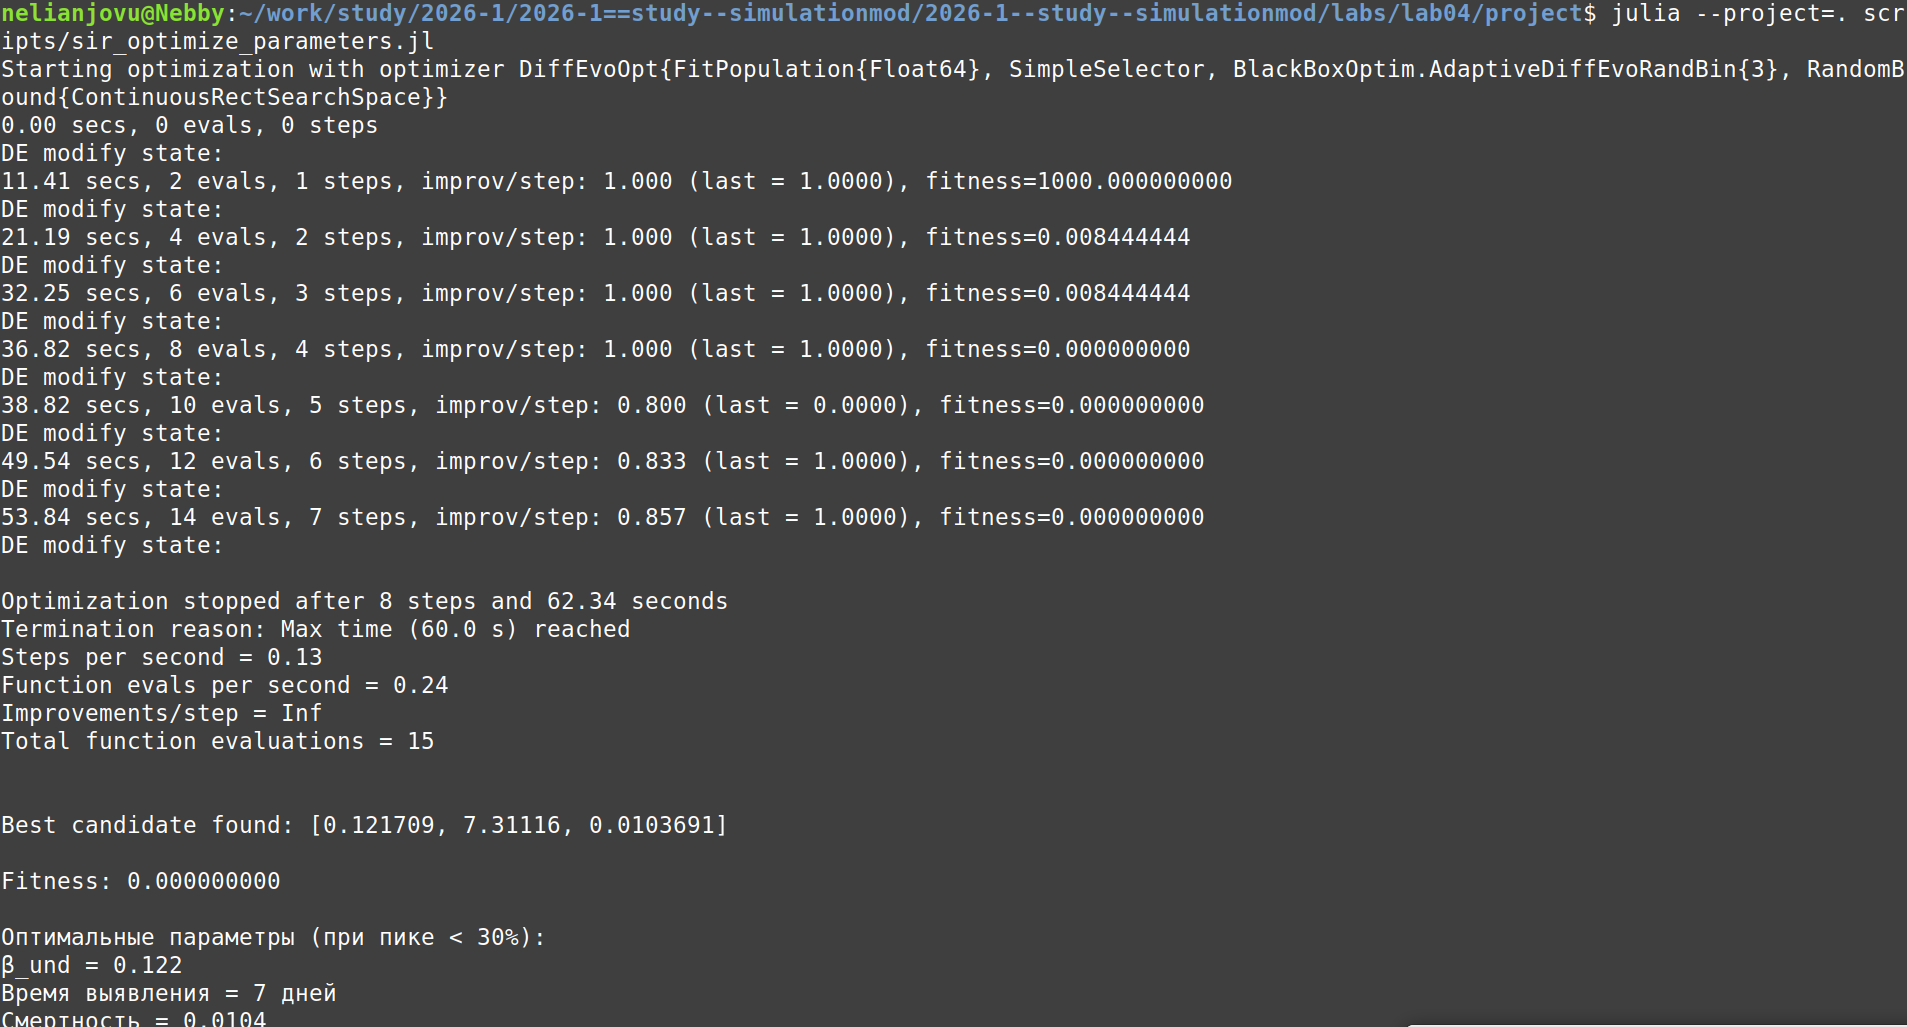
\includegraphics[width=0.7\textwidth,height=\textheight]{image/pic34.png}

}

\caption{\label{fig-030}оптимизация параметров}

\end{figure}%

После этого я создала текст на основе литературного кода: чистого кода,
записной книжки jupyter и документации в формате Quarto. Я запускала все
ячейки в файле jupyter notebook, и все работает хорошо(рис.31)

\begin{figure}

\centering{

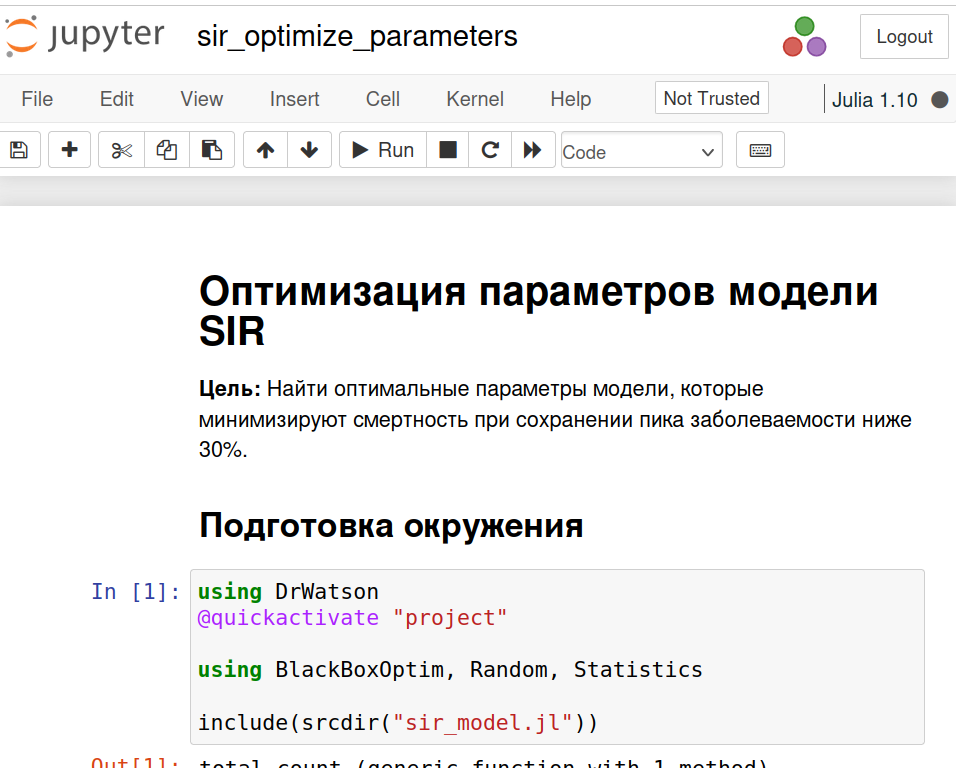
\includegraphics[width=0.7\textwidth,height=\textheight]{image/pic35.png}

}

\caption{\label{fig-031}создание файлов}

\end{figure}%

\textbf{\emph{Ниже приведен код, результаты расчетов и графики для кода
в файле scripts/sir\_optimize\_parameters.jl.qmd}}

\chapter{Оптимизация параметров модели
SIR}\label{ux43eux43fux442ux438ux43cux438ux437ux430ux446ux438ux44f-ux43fux430ux440ux430ux43cux435ux442ux440ux43eux432-ux43cux43eux434ux435ux43bux438-sir}

\textbf{Цель:} Найти оптимальные параметры модели, которые минимизируют
смертность при сохранении пика заболеваемости ниже 30\%.

\section{Подготовка
окружения}\label{ux43fux43eux434ux433ux43eux442ux43eux432ux43aux430-ux43eux43aux440ux443ux436ux435ux43dux438ux44f-2}

\begin{Shaded}
\begin{Highlighting}[]
\ImportTok{using} \BuiltInTok{DrWatson}
\PreprocessorTok{@quickactivate} \StringTok{"project"}

\ImportTok{using} \BuiltInTok{BlackBoxOptim}\NormalTok{, }\BuiltInTok{Random}\NormalTok{, }\BuiltInTok{Statistics}

\FunctionTok{include}\NormalTok{(}\FunctionTok{srcdir}\NormalTok{(}\StringTok{"sir\_model.jl"}\NormalTok{))}
\end{Highlighting}
\end{Shaded}

\begin{verbatim}
┌ Warning: DrWatson could not find find a project file by recursively checking given `dir` and its parents. Returning `nothing` instead.
│ (given dir: /home/nelianjovu)
└ @ DrWatson ~/.julia/packages/DrWatson/2QF5p/src/project_setup.jl:84
\end{verbatim}

\begin{verbatim}
total_count (generic function with 1 method)
\end{verbatim}

\section{Целевая функция с
ограничением}\label{ux446ux435ux43bux435ux432ux430ux44f-ux444ux443ux43dux43aux446ux438ux44f-ux441-ux43eux433ux440ux430ux43dux438ux447ux435ux43dux438ux435ux43c}

Функция получает три параметра и возвращает долю умерших, если пик
заболеваемости ниже 30\%. В противном случае возвращает большой штраф. -
\textbf{x{[}1{]}}: β\_und - коэффициент заразности - \textbf{x{[}2{]}}:
detection\_time - время до выявления заболевания (дни) -
\textbf{x{[}3{]}}: death\_rate - вероятность летального исхода

\begin{Shaded}
\begin{Highlighting}[]
\KeywordTok{function} \FunctionTok{cost\_multi}\NormalTok{(x)}
\NormalTok{    replicates }\OperatorTok{=} \FloatTok{3}
\NormalTok{    peak\_vals }\OperatorTok{=} \DataTypeTok{Float64}\NormalTok{[]}
\NormalTok{    dead\_vals }\OperatorTok{=} \DataTypeTok{Float64}\NormalTok{[]}

    \ControlFlowTok{for}\NormalTok{ rep }\OperatorTok{=} \FloatTok{1}\OperatorTok{:}\NormalTok{replicates}
\NormalTok{        model }\OperatorTok{=} \FunctionTok{initialize\_sir}\NormalTok{(;}
\NormalTok{            Ns }\OperatorTok{=}\NormalTok{ [}\FloatTok{1000}\NormalTok{, }\FloatTok{1000}\NormalTok{, }\FloatTok{1000}\NormalTok{],}
\NormalTok{            β\_und }\OperatorTok{=} \FunctionTok{fill}\NormalTok{(x[}\FloatTok{1}\NormalTok{], }\FloatTok{3}\NormalTok{),}
\NormalTok{            β\_det }\OperatorTok{=} \FunctionTok{fill}\NormalTok{(x[}\FloatTok{1}\NormalTok{]}\OperatorTok{/}\FloatTok{10}\NormalTok{, }\FloatTok{3}\NormalTok{),}
\NormalTok{            infection\_period }\OperatorTok{=} \FloatTok{14}\NormalTok{,}
\NormalTok{            detection\_time }\OperatorTok{=} \FunctionTok{round}\NormalTok{(}\DataTypeTok{Int}\NormalTok{, x[}\FloatTok{2}\NormalTok{]),}
\NormalTok{            death\_rate }\OperatorTok{=}\NormalTok{ x[}\FloatTok{3}\NormalTok{],}
\NormalTok{            reinfection\_probability }\OperatorTok{=} \FloatTok{0.1}\NormalTok{,}
\NormalTok{            Is }\OperatorTok{=}\NormalTok{ [}\FloatTok{0}\NormalTok{, }\FloatTok{0}\NormalTok{, }\FloatTok{1}\NormalTok{],}
\NormalTok{            seed }\OperatorTok{=} \FloatTok{42} \OperatorTok{+}\NormalTok{ rep,}
\NormalTok{            n\_steps }\OperatorTok{=} \FloatTok{100}\NormalTok{,}
\NormalTok{        )}

        \FunctionTok{infected\_frac}\NormalTok{(model) }\OperatorTok{=} \FunctionTok{count}\NormalTok{(a.status }\OperatorTok{==} \OperatorTok{:}\NormalTok{I }\ControlFlowTok{for}\NormalTok{ a }\KeywordTok{in} \FunctionTok{allagents}\NormalTok{(model)) }\OperatorTok{/} \FunctionTok{nagents}\NormalTok{(model)}

\NormalTok{        peak\_infected }\OperatorTok{=} \FloatTok{0.0}

        \ControlFlowTok{for}\NormalTok{ step }\OperatorTok{=} \FloatTok{1}\OperatorTok{:}\FloatTok{100}
\NormalTok{            Agents.}\FunctionTok{step!}\NormalTok{(model, }\FloatTok{1}\NormalTok{)}
\NormalTok{            frac }\OperatorTok{=} \FunctionTok{infected\_frac}\NormalTok{(model)}
            \ControlFlowTok{if}\NormalTok{ frac }\OperatorTok{\textgreater{}}\NormalTok{ peak\_infected}
\NormalTok{                peak\_infected }\OperatorTok{=}\NormalTok{ frac}
            \ControlFlowTok{end}
        \ControlFlowTok{end}

\NormalTok{        dead\_count }\OperatorTok{=} \FloatTok{3000} \OperatorTok{{-}} \FunctionTok{nagents}\NormalTok{(model)}

        \FunctionTok{push!}\NormalTok{(peak\_vals, peak\_infected)}
        \FunctionTok{push!}\NormalTok{(dead\_vals, dead\_count }\OperatorTok{/} \FloatTok{3000}\NormalTok{)}
    \ControlFlowTok{end}

\NormalTok{    mean\_peak }\OperatorTok{=} \FunctionTok{mean}\NormalTok{(peak\_vals)}
\NormalTok{    mean\_deaths }\OperatorTok{=} \FunctionTok{mean}\NormalTok{(dead\_vals)}

    \ControlFlowTok{if}\NormalTok{ mean\_peak }\OperatorTok{\textgreater{}} \FloatTok{0.30} \CommentTok{\# Штраф: если пик \textgreater{} 30\%, возвращаем большое значение}
        \ControlFlowTok{return} \FloatTok{1000.0}
    \ControlFlowTok{end}

    \ControlFlowTok{return}\NormalTok{ mean\_deaths}
\ControlFlowTok{end}
\end{Highlighting}
\end{Shaded}

\begin{verbatim}
cost_multi (generic function with 1 method)
\end{verbatim}

\section{Запуск
оптимизации}\label{ux437ux430ux43fux443ux441ux43a-ux43eux43fux442ux438ux43cux438ux437ux430ux446ux438ux438}

Используем эволюционный алгоритм для поиска оптимальных параметров.

\begin{Shaded}
\begin{Highlighting}[]
\NormalTok{result }\OperatorTok{=} \FunctionTok{bboptimize}\NormalTok{(}
\NormalTok{    cost\_multi,}
\NormalTok{    Method }\OperatorTok{=} \OperatorTok{:}\NormalTok{adaptive\_de\_rand\_1\_bin,}
\NormalTok{    SearchRange }\OperatorTok{=}\NormalTok{ [}
\NormalTok{        (}\FloatTok{0.1}\NormalTok{, }\FloatTok{1.0}\NormalTok{),   }\CommentTok{\# β\_und}
\NormalTok{        (}\FloatTok{3.0}\NormalTok{, }\FloatTok{14.0}\NormalTok{),  }\CommentTok{\# detection\_time}
\NormalTok{        (}\FloatTok{0.01}\NormalTok{, }\FloatTok{0.1}\NormalTok{),  }\CommentTok{\# death\_rate}
\NormalTok{    ],}
\NormalTok{    NumDimensions }\OperatorTok{=} \FloatTok{3}\NormalTok{,}
\NormalTok{    MaxTime }\OperatorTok{=} \FloatTok{60}\NormalTok{,}
\NormalTok{    PopulationSize }\OperatorTok{=} \FloatTok{20}\NormalTok{,}
\NormalTok{    TraceMode }\OperatorTok{=} \OperatorTok{:}\NormalTok{none,}
\NormalTok{)}
\end{Highlighting}
\end{Shaded}

\begin{verbatim}
Starting optimization with optimizer DiffEvoOpt{FitPopulation{Float64}, SimpleSelector, BlackBoxOptim.AdaptiveDiffEvoRandBin{3}, RandomBound{ContinuousRectSearchSpace}}
0.00 secs, 0 evals, 0 steps
DE modify state:
7.67 secs, 2 evals, 1 steps, improv/step: 1.000 (last = 1.0000), fitness=0.004222222
DE modify state:
26.68 secs, 4 evals, 2 steps, improv/step: 1.000 (last = 1.0000), fitness=0.004222222
DE modify state:
32.78 secs, 5 evals, 3 steps, improv/step: 0.667 (last = 0.0000), fitness=0.004222222
DE modify state:
51.54 secs, 7 evals, 4 steps, improv/step: 0.750 (last = 1.0000), fitness=0.004222222
DE modify state:
59.27 secs, 9 evals, 5 steps, improv/step: 0.800 (last = 1.0000), fitness=0.004222222
DE modify state:

Optimization stopped after 6 steps and 63.46 seconds
Termination reason: Max time (60.0 s) reached
Steps per second = 0.09
Function evals per second = 0.17
Improvements/step = Inf
Total function evaluations = 11


Best candidate found: [0.149987, 9.27602, 0.0734177]

Fitness: 0.000888889
\end{verbatim}

\begin{verbatim}
BlackBoxOptim.OptimizationResults("adaptive_de_rand_1_bin", "Max time (60.0 s) reached", 6, 1.775325590109846e9, 63.46448493003845, ParamsDictChain[ParamsDictChain[Dict{Symbol, Any}(:NumDimensions => 3, :MaxTime => 60.0, :SearchRange => [(0.1, 1.0), (3.0, 14.0), (0.01, 0.1)], :TraceMode => :none, :Method => :adaptive_de_rand_1_bin, :MaxFuncEvals => 0, :MaxSteps => 0, :PopulationSize => 20),Dict{Symbol, Any}()],Dict{Symbol, Any}(:CallbackInterval => -1.0, :TargetFitness => nothing, :TraceMode => :compact, :FitnessScheme => ScalarFitnessScheme{true}(), :MinDeltaFitnessTolerance => 1.0e-50, :NumDimensions => :NotSpecified, :FitnessTolerance => 1.0e-8, :TraceInterval => 0.5, :MaxStepsWithoutProgress => 10000, :MaxSteps => 10000…)], 11, ScalarFitnessScheme{true}(), BlackBoxOptim.TopListArchiveOutput{Float64, Vector{Float64}}(0.0008888888888888888, [0.1499872815535305, 9.276015132332892, 0.07341767096260449]), BlackBoxOptim.PopulationOptimizerOutput{FitPopulation{Float64}}(FitPopulation{Float64}([0.8510502853440417 0.9567459290089728 … 0.9902209350317313 0.1499872815535305; 11.440742448528745 13.845288300398522 … 9.296289268944808 9.276015132332892; 0.01979201240702558 0.04380412460591625 … 0.07024572464924622 0.07341767096260449], NaN, [NaN, 1000.0, NaN, NaN, NaN, NaN, NaN, NaN, NaN, NaN, NaN, 0.004222222222222222, 1000.0, NaN, NaN, NaN, NaN, NaN, 1000.0, NaN], 0, BlackBoxOptim.Candidate{Float64}[BlackBoxOptim.Candidate{Float64}([0.1499872815535305, 9.276015132332892, 0.07341767096260449], 20, 0.0008888888888888888, BlackBoxOptim.AdaptiveDiffEvoRandBin{3}(BlackBoxOptim.AdaptiveDiffEvoParameters(BlackBoxOptim.BimodalCauchy(Distributions.Cauchy{Float64}(μ=0.65, σ=0.1), Distributions.Cauchy{Float64}(μ=1.0, σ=0.1), 0.5, false, true), BlackBoxOptim.BimodalCauchy(Distributions.Cauchy{Float64}(μ=0.1, σ=0.1), Distributions.Cauchy{Float64}(μ=0.95, σ=0.1), 0.5, false, true), [0.6702416866808238, 0.969362766972783, 0.54698144215416, 0.6807751874500878, 0.7821812806241542, 0.6681254115257717, 1.0, 0.8683708758078881, 0.6513131014735265, 1.0, 1.0, 0.6147755924254479, 0.621509393012441, 0.42388569101359164, 0.7549016333595735, 0.8829681065577386, 0.7225541558998566, 0.9850678987687417, 0.6443120727206095, 0.6941657396609868], [0.29977084132383414, 1.0, 1.0, 0.064766722414528, 0.8669169598591087, 0.8264695588438555, 0.8603023197112094, 1.0, 0.9160326963596187, 0.08072910099733321, 0.9121382862927195, 1.0, 0.1089785772147602, 0.17827991760290043, 0.13569980414750246, 0.25223983057439003, 0.8512155105723048, 0.6143680681369716, 0.7081010856287089, 0.9525790196453883])), 0), BlackBoxOptim.Candidate{Float64}([0.23745850318197334, 13.736389400955401, 0.054209373448924576], 20, 1000.0, BlackBoxOptim.AdaptiveDiffEvoRandBin{3}(BlackBoxOptim.AdaptiveDiffEvoParameters(BlackBoxOptim.BimodalCauchy(Distributions.Cauchy{Float64}(μ=0.65, σ=0.1), Distributions.Cauchy{Float64}(μ=1.0, σ=0.1), 0.5, false, true), BlackBoxOptim.BimodalCauchy(Distributions.Cauchy{Float64}(μ=0.1, σ=0.1), Distributions.Cauchy{Float64}(μ=0.95, σ=0.1), 0.5, false, true), [0.6702416866808238, 0.969362766972783, 0.54698144215416, 0.6807751874500878, 0.7821812806241542, 0.6681254115257717, 1.0, 0.8683708758078881, 0.6513131014735265, 1.0, 1.0, 0.6147755924254479, 0.621509393012441, 0.42388569101359164, 0.7549016333595735, 0.8829681065577386, 0.7225541558998566, 0.9850678987687417, 0.6443120727206095, 0.6941657396609868], [0.29977084132383414, 1.0, 1.0, 0.064766722414528, 0.8669169598591087, 0.8264695588438555, 0.8603023197112094, 1.0, 0.9160326963596187, 0.08072910099733321, 0.9121382862927195, 1.0, 0.1089785772147602, 0.17827991760290043, 0.13569980414750246, 0.25223983057439003, 0.8512155105723048, 0.6143680681369716, 0.7081010856287089, 0.9525790196453883])), 0)], Base.Threads.SpinLock(0))))
\end{verbatim}

\section{Результаты
оптимизации}\label{ux440ux435ux437ux443ux43bux44cux442ux430ux442ux44b-ux43eux43fux442ux438ux43cux438ux437ux430ux446ux438ux438}

\begin{Shaded}
\begin{Highlighting}[]
\NormalTok{best }\OperatorTok{=} \FunctionTok{best\_candidate}\NormalTok{(result)}
\NormalTok{fitness }\OperatorTok{=} \FunctionTok{best\_fitness}\NormalTok{(result)}

\FunctionTok{println}\NormalTok{(}\StringTok{"Оптимальные параметры (при пике \textless{} 30\%):"}\NormalTok{)}
\FunctionTok{println}\NormalTok{(}\StringTok{"β\_und = }\SpecialCharTok{$}\NormalTok{(}\FunctionTok{round}\NormalTok{(best[}\FloatTok{1}\NormalTok{], digits}\OperatorTok{=}\FloatTok{3}\NormalTok{))}\StringTok{"}\NormalTok{)}
\FunctionTok{println}\NormalTok{(}\StringTok{"Время выявления = }\SpecialCharTok{$}\NormalTok{(}\FunctionTok{round}\NormalTok{(}\DataTypeTok{Int}\NormalTok{, best[}\FloatTok{2}\NormalTok{]))}\StringTok{ дней"}\NormalTok{)}
\FunctionTok{println}\NormalTok{(}\StringTok{"Смертность = }\SpecialCharTok{$}\NormalTok{(}\FunctionTok{round}\NormalTok{(best[}\FloatTok{3}\NormalTok{], digits}\OperatorTok{=}\FloatTok{4}\NormalTok{))}\StringTok{"}\NormalTok{)}
\FunctionTok{println}\NormalTok{(}\StringTok{"Доля умерших: }\SpecialCharTok{$}\NormalTok{(}\FunctionTok{round}\NormalTok{(fitness}\OperatorTok{*}\FloatTok{100}\NormalTok{, digits}\OperatorTok{=}\FloatTok{2}\NormalTok{))}\StringTok{\%"}\NormalTok{)}
\end{Highlighting}
\end{Shaded}

\begin{verbatim}
Оптимальные параметры (при пике < 30%):
β_und = 0.15
Время выявления = 9 дней
Смертность = 0.0734
Доля умерших: 0.09%
\end{verbatim}

\section{Сохранение
результатов}\label{ux441ux43eux445ux440ux430ux43dux435ux43dux438ux435-ux440ux435ux437ux443ux43bux44cux442ux430ux442ux43eux432-3}

\begin{Shaded}
\begin{Highlighting}[]
\FunctionTok{save}\NormalTok{(}\FunctionTok{datadir}\NormalTok{(}\StringTok{"optimization\_result.jld2"}\NormalTok{), }\FunctionTok{Dict}\NormalTok{(}\StringTok{"best"} \OperatorTok{=\textgreater{}}\NormalTok{ best, }\StringTok{"fitness"} \OperatorTok{=\textgreater{}}\NormalTok{ fitness))}
\end{Highlighting}
\end{Shaded}

\section{Результаты}\label{ux440ux435ux437ux443ux43bux44cux442ux430ux442ux44b}

Я создала файл sir\_visualize\_dynamics.jl и копирую в него скрипт из
лабораторного руководства. Этот скрипт загружает результаты
параметрического сканирования и строит единый составной график,
объединяющий три панели: пик эпидемии и конечная доля инфицированных;
число умерших; доля выздоровевших.(рис.32)

\begin{figure}

\centering{

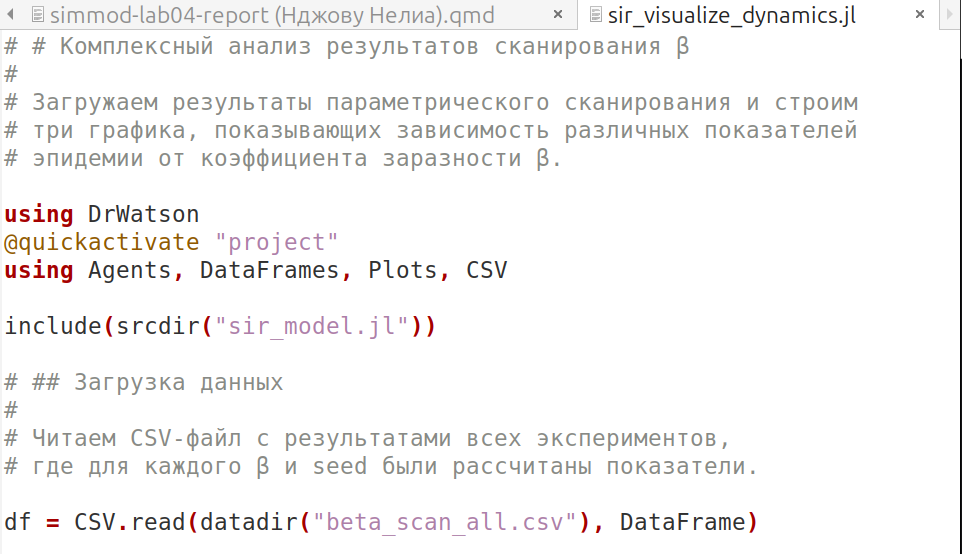
\includegraphics[width=0.7\textwidth,height=\textheight]{image/pic36.png}

}

\caption{\label{fig-032}визуализация результатов}

\end{figure}%

Я запустила его, и все заработало, я получила график ниже. График
пиковой инфицированности в сравнении с \(\beta\) показывает, сколько
людей заболевает в самый неподходящий момент. График смертности в
сравнении с \(\beta\) показывает, сколько людей умирает. График
окончательного выздоровления в сравнении с \(\beta\) показывает, сколько
людей выживают и приобретают иммунитет(рис.33)

\begin{figure}

\centering{

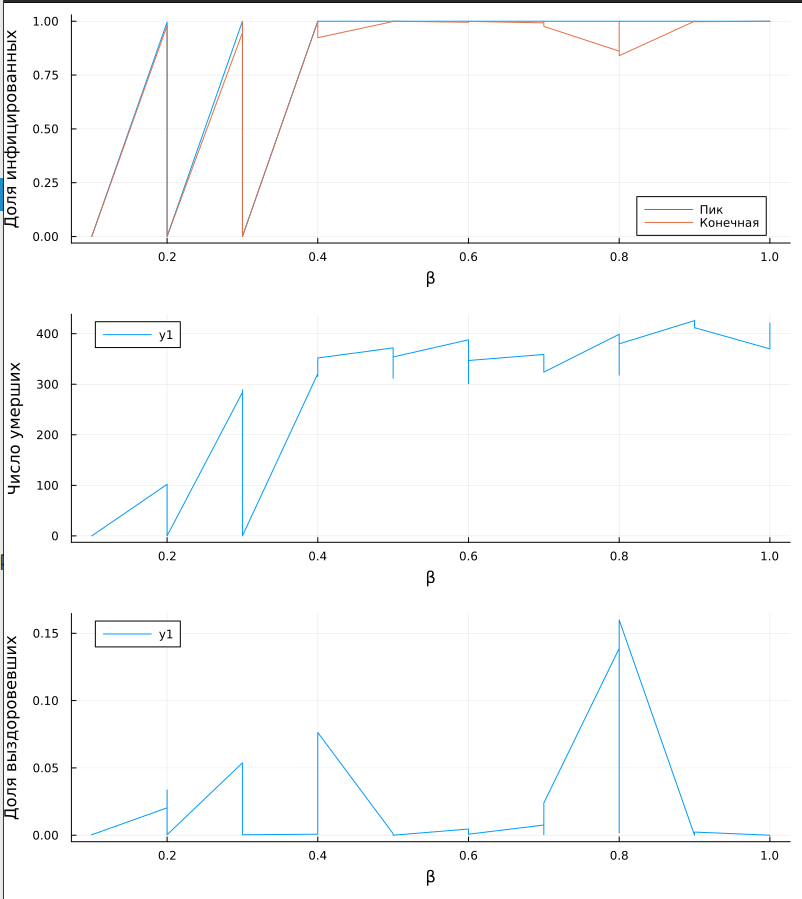
\includegraphics[width=0.7\textwidth,height=\textheight]{image/pic37.png}

}

\caption{\label{fig-033}График}

\end{figure}%

После этого я создала текст на основе литературного кода: чистого кода,
записной книжки jupyter и документации в формате Quarto. Я запускала все
ячейки в файле jupyter notebook, и все работает хорошо(рис.34)

\begin{figure}

\centering{

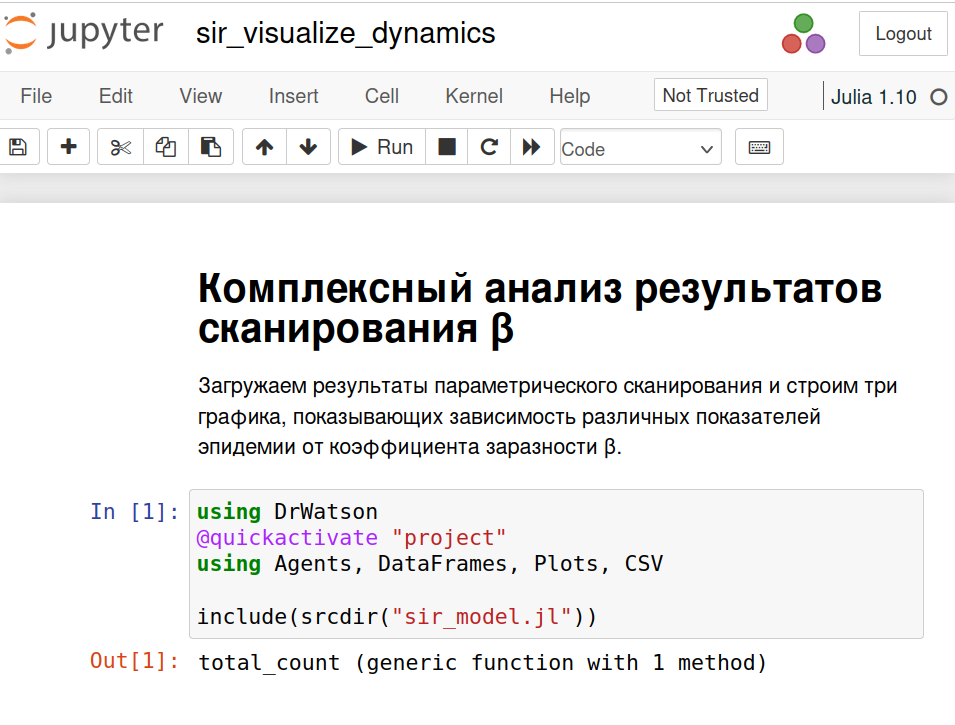
\includegraphics[width=0.7\textwidth,height=\textheight]{image/pic38.png}

}

\caption{\label{fig-034}создание файлов}

\end{figure}%

\textbf{\emph{Ниже приведен код, результаты расчетов и графики для кода
в файле scripts/sir\_visualize\_dynamics.jl.qmd}}

\chapter{Комплексный анализ результатов сканирования
β}\label{ux43aux43eux43cux43fux43bux435ux43aux441ux43dux44bux439-ux430ux43dux430ux43bux438ux437-ux440ux435ux437ux443ux43bux44cux442ux430ux442ux43eux432-ux441ux43aux430ux43dux438ux440ux43eux432ux430ux43dux438ux44f-ux3b2}

Загружаем результаты параметрического сканирования и строим три графика,
показывающих зависимость различных показателей эпидемии от коэффициента
заразности β.

\begin{Shaded}
\begin{Highlighting}[]
\ImportTok{using} \BuiltInTok{DrWatson}
\PreprocessorTok{@quickactivate} \StringTok{"project"}
\ImportTok{using} \BuiltInTok{Agents}\NormalTok{, }\BuiltInTok{DataFrames}\NormalTok{, }\BuiltInTok{Plots}\NormalTok{, }\BuiltInTok{CSV}

\FunctionTok{include}\NormalTok{(}\FunctionTok{srcdir}\NormalTok{(}\StringTok{"sir\_model.jl"}\NormalTok{))}
\end{Highlighting}
\end{Shaded}

\begin{verbatim}
┌ Warning: DrWatson could not find find a project file by recursively checking given `dir` and its parents. Returning `nothing` instead.
│ (given dir: /home/nelianjovu)
└ @ DrWatson ~/.julia/packages/DrWatson/2QF5p/src/project_setup.jl:84
\end{verbatim}

\begin{verbatim}
total_count (generic function with 1 method)
\end{verbatim}

\section{Загрузка
данных}\label{ux437ux430ux433ux440ux443ux437ux43aux430-ux434ux430ux43dux43dux44bux445}

Читаем CSV-файл с результатами всех экспериментов, где для каждого β и
seed были рассчитаны показатели.

\begin{Shaded}
\begin{Highlighting}[]
\NormalTok{df }\OperatorTok{=}\NormalTok{ CSV.}\FunctionTok{read}\NormalTok{(}\FunctionTok{datadir}\NormalTok{(}\StringTok{"beta\_scan\_all.csv"}\NormalTok{), DataFrame)}
\end{Highlighting}
\end{Shaded}

\begin{tabular}{r|cccccccc}
    & n\_steps & final\_rec & Ns & death\_rate & Is & beta & infection\_period & \\
    \hline
    & Int64 & Float64 & String31 & Float64 & String15 & Float64 & Int64 & \\
    \hline
    1 & 100 & 0.000333333 & [1000, 1000, 1000] & 0.02 & [0, 0, 1] & 0.1 & 14 & $\dots$ \\
    2 & 100 & 0.000666667 & [1000, 1000, 1000] & 0.02 & [0, 0, 1] & 0.1 & 14 & $\dots$ \\
    3 & 100 & 0.000333333 & [1000, 1000, 1000] & 0.02 & [0, 0, 1] & 0.1 & 14 & $\dots$ \\
    4 & 100 & 0.0203589 & [1000, 1000, 1000] & 0.02 & [0, 0, 1] & 0.2 & 14 & $\dots$ \\
    5 & 100 & 0.0335846 & [1000, 1000, 1000] & 0.02 & [0, 0, 1] & 0.2 & 14 & $\dots$ \\
    6 & 100 & 0.000333333 & [1000, 1000, 1000] & 0.02 & [0, 0, 1] & 0.2 & 14 & $\dots$ \\
    7 & 100 & 0.0537555 & [1000, 1000, 1000] & 0.02 & [0, 0, 1] & 0.3 & 14 & $\dots$ \\
    8 & 100 & 0.0011066 & [1000, 1000, 1000] & 0.02 & [0, 0, 1] & 0.3 & 14 & $\dots$ \\
    9 & 100 & 0.000333333 & [1000, 1000, 1000] & 0.02 & [0, 0, 1] & 0.3 & 14 & $\dots$ \\
    10 & 100 & 0.000746547 & [1000, 1000, 1000] & 0.02 & [0, 0, 1] & 0.4 & 14 & $\dots$ \\
    11 & 100 & 0.0260708 & [1000, 1000, 1000] & 0.02 & [0, 0, 1] & 0.4 & 14 & $\dots$ \\
    12 & 100 & 0.076284 & [1000, 1000, 1000] & 0.02 & [0, 0, 1] & 0.4 & 14 & $\dots$ \\
    13 & 100 & 0.00114155 & [1000, 1000, 1000] & 0.02 & [0, 0, 1] & 0.5 & 14 & $\dots$ \\
    14 & 100 & 0.0 & [1000, 1000, 1000] & 0.02 & [0, 0, 1] & 0.5 & 14 & $\dots$ \\
    15 & 100 & 0.0 & [1000, 1000, 1000] & 0.02 & [0, 0, 1] & 0.5 & 14 & $\dots$ \\
    16 & 100 & 0.00459418 & [1000, 1000, 1000] & 0.02 & [0, 0, 1] & 0.6 & 14 & $\dots$ \\
    17 & 100 & 0.000370508 & [1000, 1000, 1000] & 0.02 & [0, 0, 1] & 0.6 & 14 & $\dots$ \\
    18 & 100 & 0.000753864 & [1000, 1000, 1000] & 0.02 & [0, 0, 1] & 0.6 & 14 & $\dots$ \\
    19 & 100 & 0.00757289 & [1000, 1000, 1000] & 0.02 & [0, 0, 1] & 0.7 & 14 & $\dots$ \\
    20 & 100 & 0.00037679 & [1000, 1000, 1000] & 0.02 & [0, 0, 1] & 0.7 & 14 & $\dots$ \\
    21 & 100 & 0.0239163 & [1000, 1000, 1000] & 0.02 & [0, 0, 1] & 0.7 & 14 & $\dots$ \\
    22 & 100 & 0.138793 & [1000, 1000, 1000] & 0.02 & [0, 0, 1] & 0.8 & 14 & $\dots$ \\
    23 & 100 & 0.00186428 & [1000, 1000, 1000] & 0.02 & [0, 0, 1] & 0.8 & 14 & $\dots$ \\
    24 & 100 & 0.159924 & [1000, 1000, 1000] & 0.02 & [0, 0, 1] & 0.8 & 14 & $\dots$ \\
    25 & 100 & 0.0 & [1000, 1000, 1000] & 0.02 & [0, 0, 1] & 0.9 & 14 & $\dots$ \\
    26 & 100 & 0.0 & [1000, 1000, 1000] & 0.02 & [0, 0, 1] & 0.9 & 14 & $\dots$ \\
    27 & 100 & 0.00231839 & [1000, 1000, 1000] & 0.02 & [0, 0, 1] & 0.9 & 14 & $\dots$ \\
    28 & 100 & 0.0 & [1000, 1000, 1000] & 0.02 & [0, 0, 1] & 1.0 & 14 & $\dots$ \\
    29 & 100 & 0.0 & [1000, 1000, 1000] & 0.02 & [0, 0, 1] & 1.0 & 14 & $\dots$ \\
    30 & 100 & 0.0 & [1000, 1000, 1000] & 0.02 & [0, 0, 1] & 1.0 & 14 & $\dots$ \\
\end{tabular}

\section{Визуализация
результатов}\label{ux432ux438ux437ux443ux430ux43bux438ux437ux430ux446ux438ux44f-ux440ux435ux437ux443ux43bux44cux442ux430ux442ux43eux432-3}

Создаём три графика: - \textbf{Пик эпидемии} и \textbf{конечная доля
инфицированных} от β - \textbf{Число умерших} от β - \textbf{Доля
выздоровевших} от β

\begin{Shaded}
\begin{Highlighting}[]
\NormalTok{p1 }\OperatorTok{=} \FunctionTok{plot}\NormalTok{(df.beta, df.peak, label }\OperatorTok{=} \StringTok{"Пик"}\NormalTok{, xlabel }\OperatorTok{=} \StringTok{"β"}\NormalTok{, ylabel }\OperatorTok{=} \StringTok{"Доля инфицированных"}\NormalTok{)}
\FunctionTok{plot!}\NormalTok{(p1, df.beta, df.final\_inf, label }\OperatorTok{=} \StringTok{"Конечная"}\NormalTok{)}

\NormalTok{p2 }\OperatorTok{=} \FunctionTok{plot}\NormalTok{(df.beta, df.deaths, xlabel }\OperatorTok{=} \StringTok{"β"}\NormalTok{, ylabel }\OperatorTok{=} \StringTok{"Число умерших"}\NormalTok{)}

\NormalTok{p3 }\OperatorTok{=} \FunctionTok{plot}\NormalTok{(df.beta, df.final\_rec, xlabel }\OperatorTok{=} \StringTok{"β"}\NormalTok{, ylabel }\OperatorTok{=} \StringTok{"Доля выздоровевших"}\NormalTok{)}
\end{Highlighting}
\end{Shaded}

\includesvg{simmod-lab04-report (Нджову Нелиа)_files/figure-pdf/cell-92-output-1.svg}

\includesvg{simmod-lab04-report (Нджову Нелиа)_files/figure-pdf/cell-92-output-2.svg}

\section{Сохранение
графика}\label{ux441ux43eux445ux440ux430ux43dux435ux43dux438ux435-ux433ux440ux430ux444ux438ux43aux430}

Объединяем три графика в один вертикальный макет и сохраняем в файл.

\begin{Shaded}
\begin{Highlighting}[]
\FunctionTok{plot}\NormalTok{(p1, p2, p3, layout }\OperatorTok{=}\NormalTok{ (}\FloatTok{3}\NormalTok{, }\FloatTok{1}\NormalTok{), size }\OperatorTok{=}\NormalTok{ (}\FloatTok{800}\NormalTok{, }\FloatTok{900}\NormalTok{))}
\FunctionTok{savefig}\NormalTok{(}\FunctionTok{plotsdir}\NormalTok{(}\StringTok{"comprehensive\_analysis.png"}\NormalTok{))}
\end{Highlighting}
\end{Shaded}

\includesvg{simmod-lab04-report (Нджову Нелиа)_files/figure-pdf/cell-93-output-1.svg}

\begin{verbatim}
"/home/nelianjovu/work/study/2026-1/2026-1==study--simulationmod/2026-1--study--simulationmod/labs/lab04/project/plots/comprehensive_analysis.png"
\end{verbatim}

\chapter{Выводы}\label{ux432ux44bux432ux43eux434ux44b}

Выполнив эту лабораторную работу, я использовала агентную модель для
моделирования SIR модель.Я провла несколько экспериментов, изменив
параметры и окружающую среду


\printbibliography


\end{document}
